\documentclass[]{tufte-book}

% ams
\usepackage{amssymb,amsmath}

\usepackage{ifxetex,ifluatex}
\usepackage{fixltx2e} % provides \textsubscript
\ifnum 0\ifxetex 1\fi\ifluatex 1\fi=0 % if pdftex
  \usepackage[T1]{fontenc}
  \usepackage[utf8]{inputenc}
\else % if luatex or xelatex
  \makeatletter
  \@ifpackageloaded{fontspec}{}{\usepackage{fontspec}}
  \makeatother
  \defaultfontfeatures{Ligatures=TeX,Scale=MatchLowercase}
  \makeatletter
  \@ifpackageloaded{soul}{
     \renewcommand\allcapsspacing[1]{{\addfontfeature{LetterSpace=15}#1}}
     \renewcommand\smallcapsspacing[1]{{\addfontfeature{LetterSpace=10}#1}}
   }{}
  \makeatother

\fi

% graphix
\usepackage{graphicx}
\setkeys{Gin}{width=\linewidth,totalheight=\textheight,keepaspectratio}

% booktabs
\usepackage{booktabs}

% url
\usepackage{url}

% hyperref
\usepackage{hyperref}

% units.
\usepackage{units}


\setcounter{secnumdepth}{2}

% citations
\usepackage{natbib}
\bibliographystyle{apalike}

% pandoc syntax highlighting

% longtable
\usepackage{longtable,booktabs}

% multiplecol
\usepackage{multicol}

% strikeout
\usepackage[normalem]{ulem}

% morefloats
\usepackage{morefloats}


% tightlist macro required by pandoc >= 1.14
\providecommand{\tightlist}{%
  \setlength{\itemsep}{0pt}\setlength{\parskip}{0pt}}

% title / author / date
\title{Improving the Reproducibility of Experimental Data Recording and Pre-Processing}
\author{Brooke Anderson, Michael Lyons, Mercedes Gonzalez-Juarrero, Marcela Henao-Tamayo, and Gregory Robertson}
\date{}

\usepackage{booktabs}
\usepackage{amsthm}
\usepackage{fontspec}
    \setmainfont{Gill Sans}
\makeatletter
\def\thm@space@setup{%
  \thm@preskip=8pt plus 2pt minus 4pt
  \thm@postskip=\thm@preskip
}
\makeatother

\begin{document}

\maketitle



{
\setcounter{tocdepth}{1}
\tableofcontents
}

\hypertarget{overview}{%
\chapter{Overview}\label{overview}}

\newthought{The recent NIH-Wide Strategic Plan} \citep{nih2016strategic}
describes an integrative view of biology and human health that includes
translational medicine, team science, and the importance of capitalizing on an
exponentially growing and increasingly complex data ecosystem \citep{nih2018data}.
Underlying this view is the need to use, share, and re-use biomedical data
generated from widely varying experimental systems and researchers. Basic
sources of biomedical data range from relatively small sets of measurements,
such as animal body weights and bacterial cell counts that may be recorded by
hand, to thousands or millions of instrument-generated data points from various
imaging, -omic, and flow cytometry experiments. In either case, there is a
generally common workflow that proceeds from measurement to data recording,
pre-processing, analysis, and interpretation. However, in practice the distinct
actions of data recording, data pre-processing, and data analysis are often
merged or combined as a single entity by the researcher using commercial or open
source spreadsheets, or as part of an often proprietary experimental measurement
system / software combination (Figure \ref{fig:workflow}), resulting in key
failure points for reproducibility at the stages of data recording and
pre-processing.

\begin{figure}
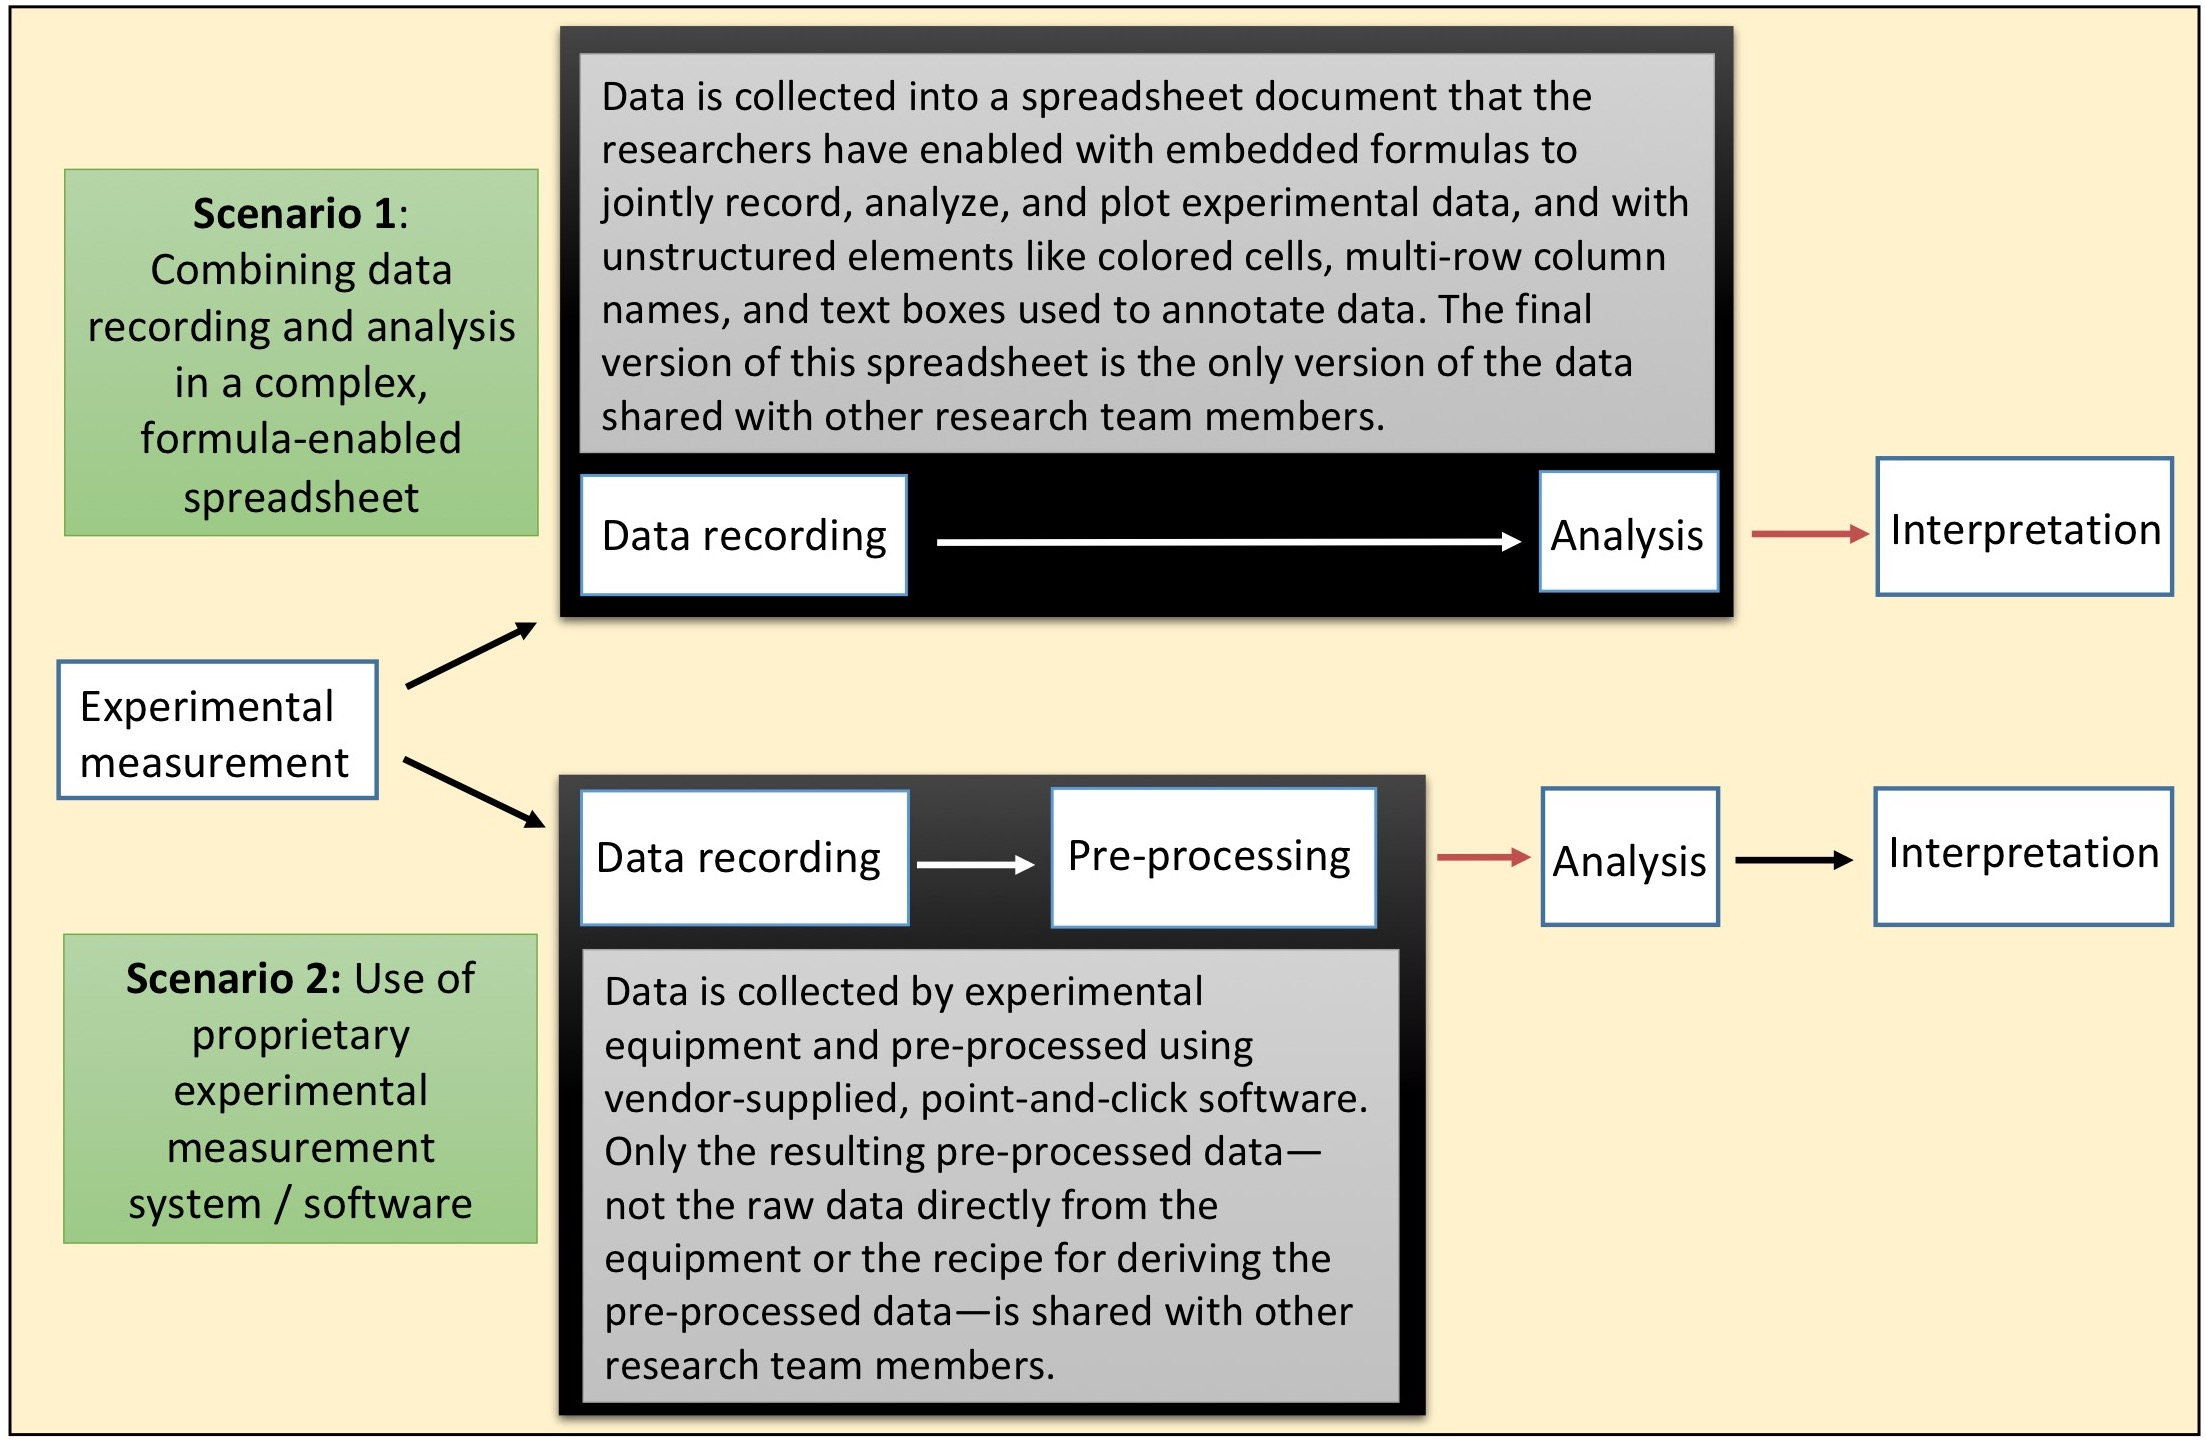
\includegraphics[width=\textwidth]{figures/existing_blackboxes} \caption[Two scenarios where 'black boxes' of non-transparent, non-reproducible data handling exist in research data workflows at the stages of data recording and pre-processing]{Two scenarios where 'black boxes' of non-transparent, non-reproducible data handling exist in research data workflows at the stages of data recording and pre-processing. These create potential points of failure for reproducible research. Red arrows indicate where data is passed to other research team members, including statisticians / data analysts, often within complex or unstructured spreadsheet files.}\label{fig:workflow}
\end{figure}

It is widely known and discussed among data scientists, mathematical modelers,
and statisticians \citep{broman2018data, krishnan2016towards} that there is
frequently a need to discard, transform, and reformat various elements of the
data shared with them by laboratory-based researchers, and that data is often
shared in an unstructured format, increasing the risks of introducing errors
through reformatting before applying more advanced computational methods.
Instead, a critical need for reproducibility is for the transparent and clear
sharing across research teams of: (1) raw data, directly from hand-recording or
directly output from experimental equipment; (2) data that has been
pre-processed as necessary (e.g., gating for flow cytometry data, feature
identification for metabolomics data), saved in a consistent, structured format,
and (3) a clear and repeatable description of how the pre-processed data was
generated from the raw data \citep{broman2018data, ellis2018share}.

To enhance data reproducibility, it is critical to create a clear separation
among data recording, data pre-processing, and data analysis---breaking up
commonly existing ``black boxes" in data handling across the research process.
Such a rigorous demarcation requires some change in the conventional
understanding and use of spreadsheets and a recognition by biomedical
researchers that recent advances in computer programming languages, especially
the R programming language, provide user-friendly and accessible tools and
concepts that can be used to extend a transparent and reproducible data workflow
to the steps of data recording and pre-processing. Among our team, we have found
that there are many common existing practices---including use of spreadsheets
with embedded formulas that concurrently record and analyze experimental data,
problematic management of project files, and reliance on proprietary,
vendor-supplied point-and-click software for data pre-processing---that can
interfere with the transparency, reproducibility, and efficiency of
laboratory-based biomedical research projects, problems that have also been
identified by others as key barriers to research reproducibility
\citep{broman2018data, bryan2018excuse, ellis2018share, marwick2018packaging}. In
these training modules, we have choosen topics that tackle barriers to
reproducibility that have straightforward, easy-to-teach solutions, but which
are still very common in biomedical laboratory-based research programs.

\hypertarget{license}{%
\section{License}\label{license}}

This book is licensed under the \href{https://creativecommons.org/licenses/by-nc-sa/4.0/}{Creative Commons
Attribution-NonCommercial-ShareAlike 4.0 International
License}, while all code in
the book is under the \href{https://opensource.org/licenses/MIT}{MIT license}.

Click on the \textbf{Next} button (or navigate using the
links at the top of the page) to continue.

\hypertarget{experimental-data-recording}{%
\chapter{Experimental Data Recording}\label{experimental-data-recording}}

\hypertarget{separating-data-recording-and-analysis}{%
\section{Separating data recording and analysis}\label{separating-data-recording-and-analysis}}

Many biomedical laboratories currently use spreadsheets---with formulas creating
underlying connections between spreadsheet cells---to jointly record, visualize,
and analyze experimental data \citep{broman2018data}. This practice impedes the
transparency and reproducibility of both data recording and data analysis. When
a research group develops and uses an evolving spreadsheet template with
embedded formulas, it leads to a data recording / analysis process that can
become extraordinarily opaque and complex. To improve the computational
reproducibility of a research project, it is critical for biomedical researchers
to learn the importance of maintaining recorded experimental data as ``read-only''
files, separating data recording from any data pre-processing or data analysis
steps \citep{broman2018data, marwick2018packaging}. Statisticians have outlined
specific methods that a laboratory-based scientist can take to ensure that data
shared in an Excel spreadsheet are shared in a reliable and reproducible way,
including avoiding macros or embedded formulas, using a separate Excel file for
each dataset, recording descriptions of variables in a separate code book rather
than in the Excel file, avoiding the use of color of the cells to encode
information, using ``NA'' to code missing values, avoiding spaces in column
headers, and avoiding splitting or merging cells \citep{ellis2018share, broman2018data}. In this module, we will describe this common practice and will
outline alternative approaches that separate the steps of data recording and
data analysis.

\textbf{Objectives.} After this module, the trainee will be able to:

\begin{itemize}
\tightlist
\item
  Explain the difference between data recording and data analysis
\item
  Understand why collecting data on spreadsheets with embedded formulas impedes
  reproducibility
\item
  List alternative approaches to improve reproducibility
\end{itemize}

\hypertarget{data-recording-versus-data-analysis}{%
\subsection{Data recording versus data analysis}\label{data-recording-versus-data-analysis}}

Many scientific laboratories use spreadsheets within their data collection
process, both to record data and to clean and analyze the data. One survey of
over 250 biomedical researchers at the University of Washington found that most
respondants used general-purpose applications like spreadsheets
\citep{anderson2007issues}, while a survey of neuroscience researchers at the
University of Newcastle similarly found that most respondents used spreadsheets
and other general-purpose software in their research \citep{altarawneh2017pilot}. A
working group on bioinformatics and data-intensive science similarly found
spreadsheets were the most common tool used across attendees
\citep{barga2011bioinformatics}.

Spreadsheets have long been an extremely popular tool, in part because they
allow people without programming experience to conduct a range of standard
computations and statistical analyses through a visual interface that is more
immediately user-friendly to non-programmers than programs with command line
interfaces. An early target for spreadsheet programs in terms of early users was
business executives, and so the programs were designed to be very simple and
easy to use---just one step up in complexity from crunching numbers on the back
of an envelope \citep{campbell2007number}. Spreadsheet programs in fact became so
popular within businesses that many attribute these programs with driving the
uptake of personal computers \citep{campbell2007number}.

Spreadsheets were innovative and rapidly adapted in part because they allowed
users to combine data recording and analysis---while previously, in business
settings, any complicated data analysis tasked needed to be outsourced to
mainframe computers and data processing teams, the initial spreadsheet program
(VisiCalc) allowed one person to quickly apply and test different models or
calculations to recorded data \citep{levy1984spreadsheet}. These spreadsheet programs
allowed non-programmers to engage with data, including data processing and
analysis tasks, that previously required programming expertise
\citep{levy1984spreadsheet}.

In some cases, a spreadsheet is used solely to record data, as a simple type of
database \citep{birch2018future}. However, biomedical researchers often use
spreadsheets to both record and analyze experimental data \citep{anderson2007issues}.
In this case, data processing and analysis is implemented through the use of
formulas and macros embedded within the spreadsheet. When a spreadsheet has
formulas or macros within it, the spreadsheet program creates an internal record
of how cells are connected through these formulas. For example, if the value in
a specific cell is converted from Fahrenheit to Celsius to fill a second cell,
and then that value is combined with other values in a column to calculate the
mean temperature across several observations, then the spreadsheet program has
internally saved how the later cells depend on the earlier ones. When you change
the value recorded in a cell of a spreadsheet, the spreadsheet program queries
this record and only recalculates the cells that depend on that cell. This
process allows the program to quickly ``react'' to any change in cell inputs,
immediately providing an update to all downstream calculations and analyses
\citep{levy1984spreadsheet}. Starting from the spreadsheet program Lotus 1-2-3,
spreadsheet programs also included \emph{macros}, ``a single computer instruction that
stands for a sequence of operations'' \citep{creeth1985microcomputer}.

Spreadsheets have become so popular in part because so many people know how to
use them, at least in basic ways, and so many people have the software on their
computers that files can be shared with the virtual guarantee that everyone will
be able to open the file on their own computer \citep{hermans2016spreadsheets}.
Spreadsheets uses the visual metaphore of a traditional gridded ledger sheet
\citep{levy1984spreadsheet}, providing an interface that is easy for users to
immediately understand and create a mental map of \citep{birch2018future, barga2011bioinformatics}. This visually clear interface also means that
spreadsheets can be printed or incorporated into other documents (Word files,
PowerPoint presentations) ``as-is'', as a workable and understandable table of
data values. In fact, some of the most popular plug-in software packages for the
early spreadsheet program Lotus 1-2-3 were programs for printing and publishing
spreadsheets \citep{campbell2007number}. This ``What You See Is What You Get''
interface was a huge advance from previous methods of data analysis for the
first spreadsheet program, VisiCalc, providing a ``window to the data'' that was
accessible to business executives and others without programming expertise
\citep{creeth1985microcomputer}. Several surveys of researchers have found that
spreadsheets were popular because of their simplicity and ease-of-use
\citep{anderson2007issues, altarawneh2017pilot, barga2011bioinformatics}. By
contrast, databases and scritped programming lanugages can be perceived as
requiring a cognitive load and lengthly training that is not worth the
investment when an easier tool is available \citep{hermans2016spreadsheets, anderson2007issues, myneni2010organization, barga2011bioinformatics, topaloglou2004biological}.

\hypertarget{hazards-of-combining-recording-and-analysis}{%
\subsection{Hazards of combining recording and analysis}\label{hazards-of-combining-recording-and-analysis}}

\textbf{Raw data often lost.}

One of the key tenets of ensuring that research is computationally reproducible
is to always keep a copy of all raw data, as well as the steps taken to get from
the raw data to a cleaned version of the data through to the results of data
analysis. However, maintaining a easily accessible copy of all original raw data
for a project is a common problem among biomedical researchers
\citep{goodman2014ten}, especially as team members move on from a laboratory group
\citep{myneni2010organization}.

The use of spreadsheets to jointly record and analyze data can contribute to
this problem. Spreadsheets allow for the immediate and embedded processing of
data. As a result, it may become very difficult to pull out the raw data
originally recorded in a spreadsheet. At the least, the combination of raw and
processed data in a spreadsheet makes it hard to identify which data points
within a spreadsheet make up the raw data and which are the result of processing
that raw data. One study of operational spreadsheets noted that:

\begin{quote}
``The data used in most spreadsheets is undocumented and there is no practical
way to check it. Even the original developer would have difficulty checking the
data.'' \citep{powell2009errors}
\end{quote}

Further, data in a spreadsheet is typically not saved as ``read-only'', so it is
possible for it to be accidentally overwritten. In situations where spreadsheets
are shared among multiple users, without ``read-only'' protection, original cell
values can easily be accidentally written over, and it may not be clear who last
changed a value, when it was changed, or why \citep{altarawneh2017pilot}.

Finally, many spreadsheets use a proprietary format. In the development of
spreadsheet programs, this use of proprietary, binary file formats helped a
software program keep users, increasing barriers for a user to switch to a new
program (since it wouldn't be able to read their old files)
\citep{campbell2007number}. However, this file format may be hard to open in the
future, as software changes and evolves \citep{michener2015ten}; by comparison, plain
text files should be widely accessible through general purpose tools regardless
of changes to proprietary software like Microsoft Excel.

\textbf{Opacity of analysis steps and potential for errors.}

Previous studies have found that errors are very common within spreadsheets
\citep{hermans2016spreadsheets}. For example, one study of 50 operational
spreadsheets found that about 90\% contained at least one error
\citep{powell2009errors}. In part, it is easier to make errors in spreadsheets and
harder to catch errors in later work with a spreadsheet because the formulas and
connections between cells aren't visible when you look at the
spreadsheet---they're behind the scenes \citep{birch2018future}. This makes it very
hard to get a clear and complete view of the pipeline of analytic steps in data
processing and analysis within a spreadsheet, as well as to discern how cells
are connected within and across sheets of the spreadsheet. As one early article on
the history of spreadsheet programs notes:

\begin{quote}
``People tend to forget that even the most elegantly crafted spreadsheet is a
house of cards, ready to collapse at the first erroneous assumption. The
spreadsheet that looks good but turns out to be tragically wrong is becoming
a familiar phenomenon.'' \citep{levy1984spreadsheet}
\end{quote}

Some characteristics of spreadsheets may heighten chances for errors. These
include high conditional complexity (i.e., lots of branching of data flow
through if / else structures), formulas that depend on a large number of cells
or that incorporate many functions \citep{hermans2016spreadsheets}. Following the
logical chain of spreadsheet formulas can be particularly difficult when several
calculations are chained in a row \citep{hermans2015enron}. Very long chains of
dependent formulas across spreadsheet cells may in some case requiring sketching
out by hand the flow of information through the spreadsheet to understand what's
going on \citep{nardi1990spreadsheet}. The use of macros can also make it
particularly hard to figure out the steps of an analysis and to diagnose and fix
any bugs in those steps \citep{nash2006spreadsheets, creeth1985microcomputer}. One
study of spreadsheets in use in real life applications noted that, ``Many
spreadsheets are so chaotically designed that auditing (especially of a few
formulas) is extremely difficult or impossible.'' \citep{powell2009errors}

In some cases, formula dependences might span across different sheets of a
spreadsheet file. For the example given above of a spreadsheet that converts
temperature from one unit to another and then averages across observations, for
example, the original temperature might be recorded in one sheet while the
converted temperature value is calculated and shown in a second sheet. These
cross-sheet dependencies can make the analysis steps even more opaque
\citep{hermans2016spreadsheets}, as a change in the cell value of one sheet might not
be immediately visible as a change in another cell on that sheet (the same is
true for spreadsheets so large that upstream and downstream cells are not
concurrently visible on screen). Other common sources of errors included
incorrect references to cells inside formulas and incorrect use of formulas
\citep{powell2009errors} or errors introduced through the common practice of copying
and pasting when developing spreadsheets \citep{hermans2016spreadsheets}.

To keep analysis steps clear, whether in scripted code or in spreadsheets or
pen-and-paper calculations, it is important to document what is being done at
each step and why \citep{goodman2014ten}. Scripted languages allow for code comments,
which are written directly into the script but not evaluated by the computer,
and so can be used to document steps within the code without changing the
operation of the code. Further, the program file itself often presents a linear,
step-by-step view of the pipeline, stored separated from the data itself
\citep{creeth1985microcomputer}. Calculations done with pen-and-paper (e.g., in a
laboratory notebook) can be annotated with text to document the steps. However,
there is evidence that spreadsheets are often poorly documented, or documented
in ways that are hard to keep track of. Before spreadsheets,

\begin{quote}
``The formulas appeared in one place and the results in another. You could see
what you were getting. That cannot be said of electronic spreadsheets, which
don't display the formulas that govern their calculations. As Mitch Kapor
explained, with electronic spreadsheets, `You can just randomly make formulas,
all of which depend on each other. And when you look at the final results, you
have no way of knowing what the rules are, unless someone tells you.'\,''
\citep{levy1984spreadsheet}
\end{quote}

Within spreadsheets, the logic and methods behind the pipeline of data
processing and analysis is often not documented, or only documented with cell
comments (hard to see as a whole) or in emails, not the spreadsheet file.
One study that investigated a large collection of spreadsheets found that most
do not include documentation explaining the logic or implementation of data
processing and analysis implemented within the spreadsheet
\citep{hermans2016spreadsheets}. A survey of neuroscience researchers at a UK
institute found that about a third of respondents included no documentation
for spreadsheets used in their research laboratories \citep{altarawneh2017pilot}.

When spreadsheet pipelines are documented, it is often through methods that are
hard to find and interpret later. One study of scientific researchers found
that, when research spreadsheets were documented, it was often through ``cell
comments'' added to specific cells in the spreadsheet, which can be hard to
interpret inclusively to understand the flow and logic of a spreadsheet as a
whole \citep{altarawneh2017pilot}. In some cases, teams discuss and document
functionality and changes in spreadsheets through email chains, passing
different versions of the spreadsheet file as attachments of emails with
discussion of the spreadsheet in the email body. One research team investigated
over 700,000 emails from employees of Enron that were released during legal
proceedings and investigated the spreadsheets attached to these emails (over
15,000 spreadsheets) as well as discussion of the spreadsheets within the emails
themselves \citep{hermans2015enron}. They found that the logic and methods of
calculations within the spreadsheets were often documented within the bodies of
emails that team members used to share and discuss spreadsheets. This means
that, if someone needs to figure out why a step was taken or identify when an
error was introduced into a spreadsheet, they may need to dig through the chain
of old emails documenting that spreadsheet, rather than being able to find the
relevant documentation within the spreadsheet's own file.

Often spreadsheets are designed, and their structure determined, by one person,
and this is often done in an \emph{ad hoc} fashion, rather than designing the
spreadsheet to follow a common structure for the research field or for the
laboratory group \citep{anderson2007issues}. Often, data processing and analysis
pipelines for spreadsheets are not carefully designed; instead, it's more
typically for spreadsheet user to start by directly entering data and formulas
without a clear overall plan \citep{altarawneh2017pilot}. Often, the person who
created the spreadsheet is the only person who fully knows how it works
\citep{myneni2010organization}, particularly if the spreadsheet includes complex
macros or a complicated structure in the analysis pipeline
\citep{creeth1985microcomputer}.

This practice creates a heavy dependence on the person who created that
spreadsheet anytime the data or results in that spreadsheet need to be
interpreted. This is particularly problematic in projects where the spreadsheet
will be shared for collaboration or adapted to be used in a future project, as
is often done in scientific research groups. One survey of neuroscience
researchers at a UK institute, for example, found that ``on average, 2--5
researchers share the same spreadsheet''. \citep{altarawneh2017pilot} In this case, it
can be hard to ``onboard'' new people to use the file, and much of the work and
knowledge about the spreadsheet can be lost when that person moves on from the
business or laboratory group \citep{creeth1985microcomputer, myneni2010organization}. If you share a spreadsheet with numerous and complex
macros and formulas included to clean and analyze the data, it can take an
extensive amount of time, and in some cases may be impossible, for the
researcher you share it with to decipher what is being done to get from the
original data input in some cells to the final results shown in others and in
graphs. Further, if others can't figure out the steps being done through macros
and formulas in a spreadsheet, they will not be able to check it for problems in
the logic of the overall analysis pipeline or for errors in the specific
formulas used within that pipeline. They also will struggle to extend and adapt
the spreadsheet to be used for other projects. These problems come up not only
when sharing with a collaborator, but also when reviewing spreadsheets that you
have previously created and used (as many have noted, your most frequent
collaborator will likely be ``future you''). In fact, one survey of biomedical
researchers at the University of Washington noted that,

\begin{quote}
``The profusion of individually created spreadsheets containing overlapping and
inconsistently updated data created a great deal of confusion within some labs.
There was little consideration to future data exchange of submission
requirements at the time of publication.'' \citep{anderson2007issues}
\end{quote}

There are methods that have been brought from more traditional programming work
into spreadsheet programming to try to help limit errors, including spreadsheet
assertions to enable testing of spreadsheets \citep{hermans2016spreadsheets}.
However, these are often not implemented, in part perhaps because many
spreadsheet users see themselves as ``end-users'', creating spreadsheets for their
own personal use rather than as something robust to future use by others, and so
don't seek out strategies adopted by ``programmers'' when creating stable tools
for others to use \citep{hermans2016spreadsheets}. In practice, though, often a
spreadsheet is used much longer, and by more people, than originally intended.
Often, the spreadsheet in this case was not designed for robust, long-term use.
From early in the history of spreadsheet programs, users have shared spreadsheet
files with interesting functionality with other users \citep{levy1984spreadsheet},
and the lifespan of a spreadsheet can be much longer than originally
intended---a spreadsheet created by one user for their own personal use can end
up being used and modified by that person or others for years
\citep{hermans2016spreadsheets}.

\textbf{Subpar software for analysis.}

While spreadsheets serve as a widely-used tool for data recording and analysis,
in many cases spreadsheets programs are poorly suited to clean and analyze
scientific data compared to other programs. As tools and interfaces continue to
develop that make other software more user-friendly to those new to programming,
scientists may want to reevaluate the costs and benefits, in terms of both time
required for training and aptness of tools, for spreadsheet programs compared to
using scripted programming languages like R and Python.

Several problems have been identified with spreadsheet programs in the context of
recording and, especially, analyzing scientific data. First, some statistical
methods may be inferior to those available in other statistical programming language.
Since the most popular spreadsheet program (Excel) is closed source, it is hard to
identify and diagnose such problems, and there is likely less of an incentive for
problems in statistical methodology to be fixed (rather than using development time
and funds to increase easier-to-see functionality in the program). Many statistical
operations require computations that cannot be perfectly achieved with a
computer, since the computer must ultimately solve many mathematical problems using
numerical approximations rather than continuous methods (e.g., calculus). The choice of
the algorithms used for these approximations heavily influence how closely a result
approximates the true answer.

A series of papers examined the quality of statistical methods in several
statistical software programs, including Excel, starting in the 1990s
\citep{mccullough1999accuracy, mccullough1999assessing, mccullough2002accuracy, mccullough2005accuracy, mccullough2008accuracy, melard2014accuracy}. In the
earliest studies, they found some concerns across all programs considered
\citep{mccullough1999accuracy, mccullough1999assessing}. One of the biggest
concerns, however, was that there was little evidence over the years that the
identified problems in Excel were resolved, or at least improved, over time
\citep{mccullough2001does, mccullough2008accuracy}. The authors note that there may
be little incentive for checking and fixing problems with algorithms for
statistical approximation in closed source software like Excel, where sales
might depend more on the more immediately evident functionality in the software,
while problems with statistical algorithms might be less evident to potential
users \citep{mccullough2001does}.

Open source software, on the other hand, offers pathways for identifying and fixing
any problems in the software, including for statistical algorithms and methods
implemented in the software's code. Since the full source code is available, researchers
can closely inspect the algorithms being used and compare them to the latest
knowledge in statistical computing methodology. Further, if an inferior algorithm is in
use, most open source software licenses allow a user to adapt and extend the software,
for example to implement better statistical algorithms.

Second, spreadsheet programs can include automated functionality that's meant to
make something easier for most users, but that might invisibly create problems
in some cases. A critical problem, for example, has been identified when using
Excel for genomics data. When Excel encounters a cell value in a format that
seems like it could be a date (e.g., ``Mar-3-06''), it will try to convert that
cell to a ``date'' class. Many software programs save date as this special ``date''
format, where it is printed and visually appears in a format like ``3-Mar-06'' but
is saved internally by the program as a number (for Microsoft Excel, the number
of days since January 1, 1900 \citep{willekens2013chronological}). By doing this, the
software can more easily undertake calculations with dates, like calculating the
number of days between two dates or which of two dates is earlier.
Bioinformatics researchers at the National Institutes of Health found that Excel
was doing this type of automatic and irreversible date conversion for 30 gene
names, including ``MAR3'' and ``APR-4'', resulting in these gene names being lost
for further analysis \citep{zeeberg2004mistaken}. Other automatic conversion problems
caused the lost of clone identifiers with composed of digits and the letter ``E''
\citep{zeeberg2004mistaken, welsh2017escape}, which were assumed to be expressing a
number using scientific notation and so automatically and irreversibly converted
to a numeric class. Further automatic conversion problems can be caused by cells
that start with an operator (e.g., ``+ control'') or with leading zeros in a
numeric identifier (e.g., ``007'') \citep{welsh2017escape}.

Avoiding this automatic date conversion required specifying that columns with
columns susceptible to these problems, including columns of gene names, should
be retained in a ``text'' class in Excel's file import process. While this
problem was originally identified and published in 2004 \citep{zeeberg2004mistaken},
along with tips to identify and avoid the problem, a study in 2016 found that
approximately a fifth of genomics papers investigated in a large-scale review
had gene name errors resulting from Excel automatic conversion, with the rate of
errors actually increasing over time \citep{ziemann2016gene}.

Finally, spreadsheet programs can be limited as analysis needs become more
complex or large \citep{topaloglou2004biological}. For example, spreadsheets can be
problematic when integrating or merging large, separate datasets
\citep{birch2018future}. This can create barriers, for example, in biological studies
seeking to integrate measurements from different instruments (e.g., flow
cytometry data with RNA-sequencing data). Further, while datasets continue to
expand in their capacity for data, for very large datasets they continue to face
limits that may be reached in practical applications \citep{birch2018future}, and
their efficiency of running data processing and analysis pipelines across large
datasets can be slow compared to code implemented with other programming
languages.

\textbf{Difficulty collaborating with statisticians.}

Modern biomedical researchers requires large teams, with statisticians and
bioinformaticians often forming a critical part of the team to enable
sophisticated processing and analysis of experimental data. However, the process
of combining data recording and analysis of experimental data, especially
through the use of spreadsheet programs, can create barriers in working across
disciplines. One group defined these issues as ``data friction'' and ``science
friction''---the extra steps and work required at each interface where data
passes, for example, from a machine to analysis or from a collaborator in one
discipline to one in a separate discipline \citep{edwards2011science}.
From a survey of scientific labs, for example, one respondent said:

\begin{quote}
``I can give data that I think are appropriate to answer a question to a
biostatistician, but when they look at it, they see it from a different point of
view. And that spreadsheet does not really encapsulate where it came from very
well, how was it generated, was it random, how was this data collected. You
would run a series of queries that you think are pertinent to what this
biostatistician would want to know. They become a part of the exploration and
not just a receiver of whatever I decided to put in my spreadsheet on that day.
What I get back is almost never fully documented in any way that I can really
understand and add more to the process.'' \citep{myneni2010organization}
\end{quote}

When collaborating with statisticians or bioinformaticians, one of the key
sources of this ``data friction'' can result from the use of spreadsheets to
jointly record and analyze experiemental data. First, spreadsheets are easy to
print or copy into another format (e.g., PowerPoint presentation, Word
document), and so researchers often design spreadsheets to be immediately
visually appealing to viewers. For example, a spreadsheet might be designed to
include hierarchically organized headers (e.g., heading and subheading, some
within a cell merged across several columns), or to show the result of a
calculation at the bottom of a column of observations (e.g., ``Total'' in the last
cell of the column) \citep{teixeira2016emergence}. Multiple separate small tables
might be included in the same sheet, with empty cells used for visual
separation, or use a ``horizontal single entry'' design , where the headers are in
the leftmost column rather than the top row \citep{teixeira2016emergence}.

These spreadsheet design choices make it much more difficult for the contents of
the spreadsheet to be read into other statistical programs. These types of data
require several extra steps in coding, in some cases fairly complex coding, with
regular expressions or logical rules needed to parse out the data and convert it
to the needed shape, before the statistical work can be done for the dataset.
This is a poor use of time for a collaborating statistician, especially if it
can be avoided through the design of the data recording template. Further, it
introduces many more chances for errors in cleaning the data.

Further, information embedded in formulas, macros, and extra formatting like
color or text boxes is lost when the spreadsheet file is input into other
programs. Spreadsheets allow users to use highlighting to represent information
(e.g., measurements for control animals shown in red, those for experiment
animals in blue) and to include information or documentation in text boxes. For
example, one survey study of biomedical researchers at the University of
Washington included this quote from a respondent: ``I have one spreadsheet that
has all of my chromosomes \ldots{} and then I've gone through and color coded it for
homozygosity and linkage.'' \citep{anderson2007issues} All the information encoded in
this sheet through color will be lost when the data from the spreadsheet is read
into another statistical program.

\hypertarget{approaches-to-separate-recording-and-analysis}{%
\subsection{Approaches to separate recording and analysis}\label{approaches-to-separate-recording-and-analysis}}

In the remaining modules in this section, we will present and describe techniques
that can be used to limit or remove these problems. First, in the module on
``Structure data'', we will walk through techniques to design data recording
formats so that data is saved in a consistent format across experiments within
a laboratory group, and in a way that removes ``data friction'' for collaboration
with statisticians or later use in scripted code. These techniques can be immediately
used to design a better spreadsheet to be used solely for data collection.

In later modules, we will discuss the use of R projects to coordinate data
recording and analysis steps within a directory, while using separate files for
data recording versus data processing and analysis. These more advanced formats
will enable the use of quality assurance / control measures like testing of data
entry and analysis functionality, better documentation of data analysis pipelines,
and easy use of version control to track projects and collaborate transparently and
with a recorded history.

{[}We will probably want to flesh this section out as we write later modules.{]}

\hypertarget{discussion-questions}{%
\subsection{Discussion questions}\label{discussion-questions}}

:w

\hypertarget{principles-and-power-of-structured-data-formats}{%
\section{Principles and power of structured data formats}\label{principles-and-power-of-structured-data-formats}}

The format in which experimental data is recorded can have a large influence on
how easy and likely it is to implement reproducibility tools in later stages of
the research workflow. Recording data in a ``structured'' format brings many
benefits. In this module, we will explain what makes a dataset ``structured'' and
why this format is a powerful tool for reproducible research.

Every extra step of data cleaning is another chance to introduce errors in
experimental biomedical data, and yet laboratory-based researchers often share
experimental data with collaborators in a format that requires extensive
additional cleaning before it can be input into data analysis
\citep{broman2018data}. Recording data in a ``structured'' format brings many
benefits for later stages of the research process, especially in terms of
improving reproducibility and reducing the probability of errors in analysis
\citep{ellis2018share}. Data that is in a structured, tabular, two-dimensional
format is substantially easier for collaborators to understand and work with,
without additional data formatting \citep{broman2018data}. Further, by using a
consistent structured format across many or all data in a research project, it
becomes much easier to create solid, well-tested code scripts for data
pre-processing and analysis and to apply those scripts consistently and
reproducibly across datasets from multiple experiments \citep{broman2018data}.
However, many biomedical researchers are unaware of this simple yet powerful
strategy in data recording and how it can improve the efficiency and
effectiveness of collaborations \citep{ellis2018share}.

\textbf{Objectives.} After this module, the trainee will be able to:

\begin{itemize}
\tightlist
\item
  List the characteristics of a structured data format
\item
  Describe benefits for research transparency and reproducibility
\item
  Outline other benefits of using a structured format when recording data
\end{itemize}

\hypertarget{data-recording-standards}{%
\subsection{Data recording standards}\label{data-recording-standards}}

For many areas of biological data, there has been a push to create standards for
how data is recorded and communicated. Standards can clarify both the \emph{content}
that should be included in a dataset, the \emph{format} in which that content is
stored, and the \emph{vocabulary} used within this data. One article names these three
facets of a data standard as the \textbf{minimum information}, \textbf{file formats}, and
\textbf{ontologies} \citep{ghosh2011software}.

\begin{quote}
``It is important to distinguish between standards that specify how to actually
do experiments and standards that specify how to describe experiments.
Recommendations such as what standard reporters (probes) should be printed on
microarrays or what quality control steps should be used in an experiment belong
to the first category. Here we focus on the standards that specify how to
describe and communicate data and information.'' \citep{brazma2006standards}
\end{quote}

Many people and organizations (including funders) are excited about the idea
of developing and using data standards, especially at the community level.
Good standards, that are widely adapted by researchers, can help in making
sure that data submitted to data repositories are used widely and that software
can be developed that is \emph{interoperable} with data from many research group's
experiments. There are also many advantages, if there are not community-level
standards for recording a certain type of data, to develop and use local
data standards for recording data from your own experiments. This section
describes the elements that go into a data standard, discusses some choices
to be made when definining a data standard (especially choices on data
structure and file formats), and some of the advantages and disadvantages
of developing and using data recording standards at both the research group
and community levels.

\begin{quote}
The first of four root causes for irreproducibility in biomedical research: ``First,
a lack of standards for data generation leads to problems with the comparability
and integration of data sets.'' \citep{waltemath2016modeling}
\end{quote}

\textbf{Ontology standards.} Although it has the most complex name, an \emph{ontology}
(sometimes called a \emph{terminology} \citep{sansone2012toward}) might be the easiest and
quickest to adapt in recording data. An ontology helps define a vocabulary that
is controlled and consistent to use that researchers can use to refer to
concepts and concrete things within an area of research. It helps researchers,
when they want to talk about an idea or thing, to use one word, and just one
word, and to ensure that it will be the same word used by other researchers when
they refer to that idea or thing. Ontologies also help to define the relationships
between ideas or concrete things in a research area \citep{ghosh2011software}, but
here we'll focus on their use in provided a consistent vocabulary to use when
recording data.

For example, when recording a dataset, what do you call a small mammal that is
often kept as a pet and that has four legs and whiskers and purrs? Do you record
this as ``cat'' or ``feline'' or maybe, depending on the animal, even ``tabby'' or
``tom'' or ``kitten''? Similarly, do you record tuberculosis as ``tuberculosis'' or
``TB'' or or maybe even ``consumption''? If you do not use the same word
consistently in a dataset to record an idea, then while a human might be able to
understand that two words should be considered equivalent, a computer will not
be able to immediately tell that ``TB'' should be treated equivalently to
``tuberculosis''.

At a larger scale, if a research community can adapt an ontology they agree to
use throughout their studies, it will make it easier to understand and integrate
datasets produced by different research laboratories. If every research group
uses the term ``cat'', then code can easily be written to extract and combine
all data recorded for cats across a large repository of experimental data.
On the other hand, if different terms are used, then it might be necessary to
first create a list of all terms used in datasets in the respository, then pick
through that list to find any terms that are exchangeable with ``cat'', then write
script to pull data with any of those terms.

Several onotologies already exist or are being created for biological and other
biomedical research \citep{ghosh2011software}. Existing community-level ontologies in
the biological sciences include {[}Gene Ontology and Systems Biology Ontology are
listed in the Ghosh et al.~paper as two examples{]}. For biomedical science,
practice, and research, the BioPortal website
(\url{http://bioportal.bioontology.org/}) provides access to almost 800 ontologies,
including several versions of the International Classification of Diseases, the
Medical Subject Headings (MESH), the National Cancer Institute Thesaurus, the
Orphanet Rare Disease Ontology and the National Center for Biotechnology
Information (NCBI) Organismal Classification. For each ontology in the BioPortal
website, the website provides a link for downloading the ontology in several
formats. If you download the ontology as a ``CSV'', you can open it in your
favorite spreadsheet program and explore how it defines specific terms to use
for each idea or thing you might need to discuss within that topic area, as well
as synonyms for some of the terms. To use an ontology when recording your own
data, just make sure you use the ontology's suggested terms in your data. For
example, if you'd like to use the Ontology for Biomedical Investigations
(\url{http://bioportal.bioontology.org/ontologies/OBI}) and you are recording how many
children a woman has had who were born alive, you should name that column of the
data ``number of live births'', not ``\# live births'' or ``live births (N)'' or
anything else. Other collections of ontologies exist for fields of scientific
research, including the Open Biological and Biomedical Ontology (OBO) Foundry
(\url{http://www.obofoundry.org/}).

If there are community-wide ontologies in your field, it is worthwhile to use
them in recording experimental data in your research group. Even better is to
not only consistently use the defined terms, but also to follow any conventions
with capitalization. While most statistical programs provide tools to change
capitalization (for example, to change all letters in a character string to
lower case), this process does require an extra step of data cleaning and an
extra chance for confusion or for errors to be introduced into data.

\textbf{Minimum information standards.} The next easiest facet of a data standard to
bring into data recording in a research group is \emph{minimum information}. Within a
data recording standard, \emph{minimum information} (sometimes also called \emph{minimum
reporting guidelines} \citep{sansone2012toward} or \emph{reporting requirements}
\citep{brazma2006standards}) specify \emph{what} should be included in a dataset
\citep{ghosh2011software}. Using minimum information standards help ensure that data
within a laboratory, or data posted to a repository, contain a number of
required elements. This makes it easier to re-use the data, either to compare it
to data that a lab has newly generated, or to combine several posted datasets to
aggregate them for a new, integrated analysis, considerations that are growing
in importance with the increasing prevalence of research repositories and
research consortia in many fields of biomedical science \citep{keller2017evolution}.

\begin{quote}
``Minimum information is a checklist of required supporting information for
datasets from different experiments. Examples include: Minimum Information About
a Microarray Experiment (MIAME), Minimum Information About a Proteomic
Experiment (MIAPE), and the Minimum Information for Biological and Biomedical
Investigations (MIBBI) project.'' \citep{ghosh2011software}
\end{quote}

\emph{Standardized file formats.} While using a standard ontology and a standard for
minimum information is a helpful start, it just means that each dataset has the
required elements \emph{somewhere}, and using a consistent vocabulary---it doesn't
specify where those elements are in the data or that they'll be in the same
place in every dataset that meets those standards. As a result, datasets that all
meet a common standard can still be very hard to combine, or to create common
data analysis scripts and tools for, since each dataset will require a different
process to pull out a given element.

Computer files serve as a way to organize data, whether that's recorded
datapoints or written documents or computer programs \citep{kernighan1984unix}. As
the programmer Paul Ford writes,

\begin{quote}
``Data is just stuff, or rather, structured stuff: The cells of a spreadsheet,
the structure of a Word document, computer programs themselves---all data.''
\citep{ford2015i}
\end{quote}

\noindent A \emph{file format} defines the rules for how the bytes in the chunk of
memory that makes up a certain file should be parsed and interpreted anytime you
want to meaningfully access and use the data within that file
\citep{murrell2009introduction}. There are many file formats you may be familiar
with---a file that ends in ``.pdf'' must be opened with a Portable Document Format
(PDF) Reader like Adobe Acrobat, or it won't make much sense (you can try this
out by trying to open a ``.pdf'' file with a text editor, like TextEdit or
Notepad). The Reader has been programmed to interpret the data in a ``.pdf'' file
based on rules defining what data is stored where in the section of computer
memory for that file. Because most ``.pdf'' files conform to the same \emph{file
format} rules, powerful software can be built that works with any file in that
format.

For certain types of biomedical data, the challenge of standardizing a format
has similarly been addressed through the use of well-defined rules for not only
the content of data, but also the way that content is \emph{structured}. This can be
standardized through \emph{standardized file formats} (sometimes also called \emph{data
exchange formats} \citep{brazma2006standards}) and often defines not only the
upper-level file format (e.g., use of a ``.csv'' file type), but also how data
within that file type should be organized. If data from different research
groups and experiments is recorded using the same file format, researchers can
develop software tools that can be repeatedly used to interpret and visualize
that data; on the other hand, if different experiments record data using
different formats, bespoke analysis scripts must be written for each separate
dataset. This is a blow not only to the efficiency of data analysis, but also a
threat to the accuracy of that analysis. If a set of tools can be developed that
will work over and over, more time can be devoted to refining those tools and
testing them for potential errors and bugs, while one-shot scripts often can't
be curated with similar care. One paper highlights the dangers that come with
working with files that don't follow a defined format:

\begin{quote}
``Beware of common pitfalls when working with \emph{ad hoc} bioinformatics formats.
Simple mistakes over minor details like file formats can consume a
disproportionate amount of time and energy to discover and fix, so mind these
details early on.'' \citep{buffalo2015bioinformatics}
\end{quote}

Some biomedical data file formats have been created to help smooth over the
transfer of data that's captured by complex equipment into software that can
analyze that data. For example, many immunological studies need to measure
immune cell populations in experiments, and to do so they use piece of
equipment called a flow cytometer that probes cells in a sample with lasers
and measures resulting intensities to determine characteristics of that cell.
The data created by this equipment is large (often measurements from {[}x{]} or more
lasers are taken for {[}x{]} cells in a single run) and somewhat complex, with a need
to record not only the intensity measurements from each laser, but also some metadata
about the equipment and characteristics of the run.
If every company that manufactured flow cytometers used a different file format for
saving the resulting data, then a different set of analysis software would need to
be developed to accompany each piece of equipment. For example, a laboratory at
a university with flow cytometers from two different companies would need licenses
for two different software programs to work with data recorded by flow cytometers,
and they would need to learn how to use each software package separately. There is a
chance that software could be developed that used shared code for data analysis, but only
if it also included separate sets of code to read in data from all types of equipment
and to reformat them to a common format.

This isn't the case, however. Instead, there is a commonly agreed on file
format that flow cytometers should use to record the data they collect, called
the the \emph{FCS file format}. This format has been defined through a series of
papers {[}refs{]}, with several separate versions as the file format has evolved
over the years. It provides clear specifications on where to save each relevant
piece of information in the block of memory devoted to the data recorded by the
flow cytometer (in some cases, leaving a slot in the file blank if no relevant
information was collected on that element). As a result, people have been able
to create software, both proprietary and open-source, that can be used with any
data recorded by a flow cytometer, regardless of which company manufacturer the
piece of equipment that was used to generate the data. Other types of biomedical
data also have standardized file formats, including {[}example popular file
formats for biomedical data{]}. In some cases these were defined by an
organization, society, or initiative (e.g., the Metabolomics Standards
Initiative) \citep{ghosh2011software}, while in some cases the file format developed
by a specific equipment manufacturer has become popular enough that it's
established itself as the standard for recording a type of data
\citep{brazma2006standards}.

For an even simpler example, thing about recording dates. The \emph{minimum
information standard} for a date might always be the same---a recorded value
must include the day of the month, month, and year. However, this information
can be \emph{structured} in a variety of ways. In many scientific data, it's common
to record this information going from the largest to smallest units, so March
12, 2006, would be recorded ``2006-03-12''. Another convention (especially in the
US) is to record the month first (e.g., ``3/12/06''), while another (more common
in Europe) is to record the day of the month first (e.g., ``12/3/06'').

If you are trying to combine data from different datasets with dates, and all
use a different structure, it's easy to see how mistakes could be introduced
unless the data is very carefully reformatted. For example, March 12 (``3-12''
with month-first, ``12-3'' with day-first) could be easily mistaken to be December
3, and vice versa. Even if errors are avoided, combining data in different
structures will take more time than combining data in the same structure,
because of the extra needs for reformatting to get all data in a common
structure.

\begin{quote}
``Vast swathes of bioscience data remain locked in esoteric formats, are
described using nonstandard terminology, lack sufficient contextual information,
or simply are never shared due to the perceived cost or futility of the
exercise.'' \citep{sansone2012toward}
\end{quote}

\hypertarget{defining-data-standards-for-a-research-group}{%
\subsection{Defining data standards for a research group}\label{defining-data-standards-for-a-research-group}}

If some of the data you record from your experiments comes from complex
equipment, like flow cytometers {[}or?{]}, you may be recording much of that data in
a standardized format without any extra effort, because that format is the
default output format for the equipment. However, you may have more control over
other data recorded from your experiments, including smaller, less complex data
recorded directly into a laboratory notebook or spreadsheet. You can derive a
number of benefits from defining and using a standard for collecting this data,
as well.

As already mentioned, for many of the complex types of biological data,
standardized file formats exist. For example, flow cytometry data is typically
collected and recorded in \emph{.fcs} files. Every piece of flow cytometry equipment
can then be built to output data in this format, and every piece of software to
analyze flow cytometry data can be built to read in this input. The \emph{.fcs} file
format species how both raw data and metadata (e.g., compensation information,
equipment details) can be saved within the file---everyone who uses that file
format knows where to store data and where to find data of a certain type.

Much of the data collected in a laboratory is smaller, less complex, or less
structured than these types of data, data that is recorded ``by hand'', often into
a laboratory notebook or a spreadsheet. One paper describes this type of data as
the output of ``traditional, low-throughput bench science'' \citep{wilkinson2016fair}.
For this data recording, the data may be written down in an \emph{ad hoc}
way---however the particular researcher doing the experiment thinks makes
sense---and that format might change with each experiment, even if many
experiments have similar data outputs. As a result, it becomes harder to create
standardized data processing and analysis scripts that work with this data or
that integrate it with more complex data types. Further, if everyone in a
laboratory sets up their spreadsheets for data recording in their own way, it is
much harder for one person in the group to look at data another person recorded
and immediately find what they need within the spreadsheet.

As a step in a better direction, the head of a research group may
designate some common formats (e.g., a spreadsheet template) that all
researchers in the group should use when recording the data from a specific type
of experiments. This provides consistency across the recorded data for the
laboratory, making easier for one lab member to quickly understand and navigate
data saved by another lab member. It also opens the possibility to create tools
or scripts that read in and analyze the data that can be re-used across multiple
experiments with minor changes. This helps improve the efficiency and
reproducibility of data analysis, visualization, and reporting steps of the
research project.

This does require some extra time commitment \citep{brazma2006standards}. First, time
is needed to design the format, and it does take a while to develop a format
that is inclusive enough that it includes a place to put all data you might want
to record for a certain type of experiment. Second, it will take some time to
teach each laboratory member what the format is and how to make sure they comply
with it when they record data.

On the flip side, the longer-term advantages of using a defined, structured
format will outweigh the short-term time investments for many laboratory groups
for frequently used data types. By creating and using a consistent structure to
record data of a certain type, members of a laboratory group can increase their
efficiency (since they do not need to re-design a data recording structure
repeatedly). They can also make it easier for downstream collaborators, like
biostatisticians and bioinformaticians, to work with their output, as those
collaborators can create tools and scripts that can be recycled across
experiments and research projects if they know the data will always come to them
in the same format. These benefits increase even more if data format standards
are created and used by a whole research field (e.g., if a standard data
recording format is always used for researchers conducting a certain type of
drug development experiment), because then the tools built at one institution
can be used at other insitutions. However, this level of field-wide coordination
can be hard to achieve, and so a more realistic immediate goal might be
formalizing data recording structures within your research group or department,
while keeping an eye out for formats that are gaining popularity as standards in
your field to adopt within your group.

One key advantage to using standardized data formats even for recording simple,
``low-throughput'' data is that everyone in the research group will be able to
understand and work with data recorded by anyone else in the group---data will
not become impenetrable once the person who recorded it leaves the group. Also,
once a group member is used to the format, the process of setting up to record
data from a new experiment will be quicker, as it won't require the effort of
deciding and setting up a \emph{de novo} format for a spreadsheet or other recording
file. Instead, a template file can be created that can be copied as a starting
point for any new data recording.

Finally, there are huge benefits further down the data analysis pipeline that
come with always recording data in the same format. If your group is working
with a statistician or data analyst, it becomes much easier for that person to
quickly understand a new file if it follows the same format as previous files.
Further, if you work with a statistician or data analyst, he or she probably
creates code scripts to read in, re-format, analyze, and visualize the data
you've shared. If you always record data using the same format, these scripts
can be reused with very little modification. This saves valuable time, and it
helps make more time for more interesting statistical analysis if your
collaborator can trim time off reading in and reformatting the data in their
statistical programming language.

One paper suggests that the balance can be found, in terms of deciding whether
the benefits of developing a standard outweigh the costs, by considering how
often data of a certain type is generated and used:

\begin{quote}
``To develop and deploy a standard creates an overhead, which can be expensive.
Standards will help only if a particular type of information has to be
exchanged often enough to pay off the development, implementation, and usage
of the standard during its lifespan.'' \citep{brazma2006standards}
\end{quote}

\hypertarget{two-dimensional-structured-data-format}{%
\subsection{Two-dimensional structured data format}\label{two-dimensional-structured-data-format}}

So far, this module has explored \emph{why} you might want to use standardized
data formats for recording experimental data. The rest of the module
aims to give you tips for how to design and define your own standardized
data formats, if you decide that is worthwhile for certain data types
recorded within your research group.

Once you commit to creating a defined, structured format, you'll need to decide
what that structure should be. There are many options here, and it's very
tempting to use a format that is easy on human eyes
\citep{buffalo2015bioinformatics}. For example, it may seem appealing to create a
format that could easily be copied and pasted into presentations and Word
documents and that will look nice in those presentation formats. To facilitate
this use, a laboratory might set up a recording format base on a spreadsheet
template that includes multiple tables of different data types on the same
sheet, or multi-level column headings.

Unfortunately, many of the characteristics that make a format attractive
to human eyes will make it harder for a computer to make sense of. For example,
if you include two tables in the same spreadsheet, it might make it easier for a
person to get a one-screen look at two small data tables. However, if you want
to read that data into a statistical program (or work with a collaborator who
would), it will likely take some complex code to try to tell the computer how to
find the second table in the spreadsheet. The same applies if you include some
blank lines at the top of the spreadsheet, or use multi-level headers, or use
``summary'' rows at the bottom of a table. Further, any information you've
included with colors or with text boxes in the spreadsheet will be lost when the
data's read into a statistical program. These design elements in a data
format make it much harder to read the data embedded in a spreadsheet into other
computer programs, including programs for more complex data analysis and
visualization, like R and Python.

\begin{quote}
``Data should be formatted in a way that facilitates computer readability. All
too often, we as humans record data in a way that maximizes its readability to
us, but takes a considerable amount of cleaning and tidying before it can be
processed by a computer. The more data (and metadata) that is computer readable,
the more we can leverage our computers to work with this data.''
\citep{buffalo2015bioinformatics}
\end{quote}

For most statistical programs, data can be easily read in from a spreadsheet if
the computer can parse it in the following way: first, read in the first row,
and assign each cell in that row as the \emph{name} of a column. Then, read in the
second row, and put each cell in the column the corresponds with the name of the
cell in the same position in the first row. Also, set the data type for that
column (e.g., number, character) based on the data type in this cell. Then, keep
reading in rows until getting to a row that's completely blank, and that will be
the end of the data. If any of the rows has more cell than the first row, then
that means that something went wrong, and should result in stopping or giving a
warning. If any of the rows have fewer cells than the first row, then that means
that there are missing data in that row, and should probably be recorded as
missing values for any cells the row is ``short'' compared to the first row.

One of the easiest format for a computer to read is therefore a two-dimensional
``box'' of data, where the first row of the spreadsheet gives the column names,
and where each row contains an equal number of entries. This type of
two-dimensional tabular structure forms the basis for several popular
``delimited'' file formats that serve as a \emph{lingua franca} across many simple
computer programs, like the comma-separated values (CSV) format, the
tab-delimited values (TSV) format, and the more general delimiter-separated
values (DSV) format, which are a common format for data exchange across
databases, spreadsheet programs, and statistical programs \citep{janssens2014data, raymond2003art, buffalo2015bioinformatics}.

\begin{quote}
``Tabular plain-text data formats are used extensively in computing. The basic
format is incrediably simple: each row (also known as a record) is kept on its
own line, and each column (also known as a field) is separate by some delimiter.''
\citep{buffalo2015bioinformatics}
\end{quote}

If you think of the computer parsing a spreadsheet as described above, hopefully
it clarifies why some spreadsheet formats would cause problems. For example, if
you have two tables in the same spreadsheet, with blank lines between them, the
computer will likely either think it's read all the data after the first table,
and so not read in any data from the second table, or it will think the data
from both tables belong in a single table, with some rows of missing data in the
center. To write the code to read in data from two tables into two separate
datasets in a statistical program, it will be necessary to write some complex
code to tell the computer how to search out the start of the second table in the
spreadsheet.

Similar problems come up if a spreadsheet diverges from a regular,
two-dimensional format, with a single row of column names to start the data.
For example, if the data uses multiple rows to create multi-level
column headers, anyone reading it into another program will need to
either skip some of the rows of the column headers, and so lose information
in the original spreadsheet, or write complex code to parse the column
headers separately, then read in the later rows with data, and then stick
the two elements back together. ``Summary'' rows at the end of a dataset
(for example, the sums or means of all values in a column) will need to
be trimmed off when the data is read into other programs, since most
of the analysis and visualization someone would want to do in another
program will calculate any summaries fresh, and will want each row of
a dataset to represent the same ``type'' and level of data (e.g., one measurement
from one animal).

For anything in a data format that requires extra coding when reading data into
another program, you are introducing a new opportunity for errors at the
interface between data recording and data analysis. If there are strong reasons
to use a format that requires these extra steps, it will still be possible to
create code to read in and parse the data in statistical programs, and if the
same format is consistently used, then scripts can be developed and thoroughly
tested to allow this. However, do keep in mind that this will be an extra
burden on any data analysis collaborators who are using a program besides a
spreadsheet program. The extra time this will require could be large, since
this code should be vetted and tested thoroughly to ensure that the data
cleaning process is not introducing errors. By contrast, if the data is
recorded in a two-dimensional format with a single row of column names as
the first row, data analysts can likely read it quickly and cleanly into
other programs, with low risks of errors in the transfer of data from the
spreadsheet.

\begin{quote}
``Cleaning data is a short-term solution, and preventing errors is promoted as
a permanent solution. The drawback to cleaning data is that the process never
ends, is costly, and may allow many errors to avoid detection.''
\citep{keller2017evolution}
\end{quote}

\hypertarget{saving-two-dimensional-structured-data-in-plain-text-file-formats}{%
\subsection{Saving two-dimensional structured data in plain text file formats}\label{saving-two-dimensional-structured-data-in-plain-text-file-formats}}

If you have recorded data in a two-dimensional structured format, you can choose
to save it in either a \emph{plain text} format or a \emph{binary} format. With a plain
text format, a file is ``human readable'' when it's opened in a text editor
\citep{hunt2000pragmatic, janssens2014data}, because each byte that encodes the file
translates to a single character \citep{murrell2009introduction}, usually using an
ASCII or Unicode encoding. Common plain text file formats used for biomedical
research include CSV and TSV files (these are distinguished only by the
character used as a delimiter---commas for CSV files versus taabs for TSV files)
\citep{buffalo2015bioinformatics}, other more complex file formats like SAM and XML
are also typically saved in plain text.

A binary file format, on the other hand, encodes data within the file using an
encoding system that differs from ANSCII or Unicode. To extract the data in a
meaningful way, a computer program must know and use rules for the encoding and
structure of that file format, and those rules will be different for each
different binary file format \citep{murrell2009introduction}. Some binary file
formats are ``open'', with all the information on these rules and encodings
available for anyone to read. On the otherhand, other binary file formats are
proprietary, without available guidance on how to interpret or use the data
stored in them when creating new software tools. Binary files, because they
don't follow the restrictions of plain text encoding and format, can encode and
organize data in a way that's often much more compressed, because it's optimized
to suit a specific type of data. This means that binary file formats can often
store more data within a certain amount of computer memory compared to plain
text file formats. Binary files can also be designed so that the computer can
find and read a specific piece of data, rather than needing to read data in
linearly from the start to the end of a file as with plain text formats. This
means that programs can often access specific bits of data much more quickly
from a binary file format that from a plain text format, making computation
processing run much faster.

However, even with the speed and size advantages of many binary file formats, it
is often worthwhile to record and save experimental data in a plain text, rather
than binary, file format. There are a number of advantages to using a plain text
format. A plain text format may take more space (in terms of computer memory)
and take longer to process within other programs; however, its benefits
typically outweigh these limitations \citep{hunt2000pragmatic}. Advantages include:
(1) humans can read the file directly \citep{hunt2000pragmatic, janssens2014data},
and should always be able to, regardless of changes in and future obsolescence
of computer programs; (2) almost all software programs for analyzing and
processing files can input plain-text files, while binary file formats often
require specialized software \citep{murrell2009introduction}; (3) the
Unix system, which has influenced many existing software programs, especially
open-source programs for data analysis and command-line tools, are based on
inputting and outputtin line-based plain-text files \citep{janssens2014data}; and (4)
plain-text files can be easily tracked with version control
\citep{hunt2000pragmatic}. These advantages might become particularly important in
cases where researchers need to combine and integrate heterogeneous data, for
example data coming from different instruments.

Another advantage of storing data in a plain text format is that it makes
version control, which we'll discuss in a later module, a much more powerful
tool. With plain text files, you can use version control to see the specific
changes to a file. With binary files, you can typically see if a file was
changed, but it's much harder to see exactly what within the file was changed.

The book \emph{The Pragmatic Programmer} highlights some of the advantages of plain
text:

\begin{quote}
``Human-readable forms of data, and self-describing data, will outlive all
other forms of data and the applications that created them. Period. As long as
the data survives, you will have a chance to be able to use it---potentially
long after the original application that wrote it is defunct. \ldots{} Even in the
future of XML-based intelligent agents that travel the wild and dangerous
Internet autonomously, negotiating data interchange among themselves, the
ubiquitous text file will still be there. In fact, in heterogeneous environments
the advantages of plain text can outweight all of the drawbacks. You need to
ensure that all parties can communicate using a common standard. Plain text is
that standard.'' \citep{hunt2000pragmatic}
\end{quote}

\noindent Paul Ford, by contrast, describes some of the disadvantages of
a binary file format, using the Photoshop file format as an example:

\begin{quote}
``A Photoshop file is a lump of binary data. It just sits there on your hard
drive. Open it in Photoshop, and there are your guides, your color swatches, and
of course, the manifold pixels of your intent. But outside of Photoshop that
file is an enigma. There is not `view source'. You can, if you're passionate,
read the standard on the web, and it's all piled in there, the history of
pictures on computers. That's when it becomes clear: only Photoshop's creator
Adobe can understand this thing.'' \citep{ford2015on}
\end{quote}

Structuring data in a gridded, two-dimensional format, as described in the last
section, will be helpful even if it is in a file format that is binary, like
Excel. However, there are added benefits to saving the structured data in a
plain text format. Older Excel spreadsheets are typically saved in a proprietary
file format (``.xls''), while more recently Excel has saved files to an open
binary format based on packaging XML files with the data (``.xlsx'' file format)
\citep{janssens2014data}. While the open proprietary format is preferable, since
tools can be developed to work with them by people other than the Microsoft
team, both file formats still face some of the limitations of binary file
formats as a way of recording experimental data. However, even if you have used
a spreadsheet program like Excel to record data, it's very easy to still save
that data in a plain text file format \citep{murrell2009introduction}. In most
spreadsheet programs, you can choose to save a file ``As CSV''.

\hypertarget{occassions-for-more-complex-data-structures-and-file-formats}{%
\subsection{Occassions for more complex data structures and file formats}\label{occassions-for-more-complex-data-structures-and-file-formats}}

There are some cases where a two-dimensional data format may not be adequate
for recording experimental data, despite this format's advantages in
improving reproducibility through later data analysis steps. Similarly,
there may be cases where a binary file format, or use of a database, will
outweigh the benefits of saving data to a plain text format. Being familiar
with different file formats can also be helpful when you need to integrate
data stored in different formats \citep{murrell2009introduction}.

\textbf{Non-tabular plain-text formats.}
First, some data has a linked or hierarchical nature, in terms of how data
points are connected through the dataset. For example, data on a family try
might have a hierarchical structure, where different numbers of children are
recorded for each parent. As another example, if you were building a dataset
describing how scientists have collaborated together as coauthors, that data
might form a network. In many cases, it is possible to structure datasets with
these types of ``non-tabular'' structure using the ``tidy data'' tabular format
described in the next section. However, in very complex cases, it may work
better to use a non-tabular data format \citep{raymond2003art}. Popular data formats
that are non-tabular include the eXtensible Markup Language (XML) and JavaScript
Object Notation (JSON) formats, both of which are well-suited for
hierarchically-structured data. You may also have data you would like to use in
XML or JSON formats if you are using web services to pull datasets from online
repositories, as open data application programming interfaces (APIs) often
return data in these formats \citep{janssens2014data}.

Another use of file formats that are plain text but meant to be streamed, rather
than read in as a whole. When reading in data stored in a delimited plain text
file, like a CSV file, a statistical program like R will typically read in all
the data and then operate on the dataset as a whole. If a data file is very
large, then reading in all the data at once might require so much memory that it
slows down processing, or even exceed the program's memory cap {[}?{]}. One strategy
is to design a data format so that the program can read in a small amount of the
file, process that piece of the data, write the result out, and remove that bit
of data from the program's memory before moving into the next portion of data
\citep{buffalo2015bioinformatics}. This \emph{streaming} approach is sometimes used with
some file formats used for biomedical research, including FASTA and FASTQ files.

\textbf{Databases.}
When research datasets include not only data that can be expressed in plain
text, but also data like images, photographs, or videos, it may be worth
considering using a database to store the data \citep{murrell2009introduction}.
Relational database managment system software, like {[}examples. MySQL?
PostgreSQL?{]} can be used to organize data in a way that records connections
(\emph{relations}) between different pieces of data and allows you to access
different combinations of that data quickly using Structured Query Language, or
\emph{SQL} \citep{ford2015i}. Further, some statistical programming languages, including
R, now have tools that allow you to directly access and work with data from a
database from within the statistical program, and in some cases using scripts
that are very similar or identical to the code that would be used if you'd read
the data into the program from a plain text file.

\begin{quote}
``The database is the unsung infrastructure of the world, the shared memory of
every corporation, and the foundation of every major web site. And they are
everywhere. Nearly every host-your-own-web-site package comes with access to a
database called MySQL; just about every cell phone has SQLite3, aa tiny,
pocket-sized database, built in.'' \citep{ford2015i}
\end{quote}

It will be more complicated to set up a database for recording experimental
data, and so it's often preferable to instead save data in plain text files
within a file directory, if the data is simple enough to allow that. However,
there are some fairly simple database solutions that are now available,
including SQLite \citep{buffalo2015bioinformatics}.

\textbf{Binary file formats.}

There are cases where it may not be best to store laboratory-generated data in a
plain text format. For example, the output from a flow cytometer is large and
would take up a lot (more) computer memory if stored in a plain text format, and
it would take much longer to read and work with the data in analysis software if
it were in that format. For very large datasets like this, it may be necessary
to use a binary data format, either for size or speed or both
\citep{kernighan1984unix, hunt2000pragmatic}. For very large biomedical datasets,
binary file formats are sometimes designed for \emph{out-of-memory approaches}
\citep{buffalo2015bioinformatics}, where a file format is designed in a way that
allows computer programs to find and read only specific pieces of data in a file
through a process called \emph{random access}, rather than needing to read the full
file into memory before a specific piece of data in the file can be accessed
(a.k.a., \emph{sequential access}) \citep{murrell2009introduction}.

\hypertarget{levels-of-standardizationresearch-group-to-research-community}{%
\subsection{Levels of standardization---research group to research community}\label{levels-of-standardizationresearch-group-to-research-community}}

Standards can operate both at the level of individual research groups and at the
level of the scientific community as a whole. The potential advantages of
community-level standards are big: they offer the chance to develop
common-purpose tools and code scripts for data analysis, as well as make it
easier to re-use and combine experimental data from previous research that is
posted in open data repositories. If a software tool can be reused, then more
time can be spent in developing and testing it, and as more people use it, bugs
and shortcomings can be identified and corrected. Community-wide standards can
lead to databases with data from different experiments, and from different
laboratory groups, structured in a way that makes it easy for other researchers
to understand each dataset, find pieces of data of interest within datasets, and
integrate different datasets \citep{lynch2008big}. Similarly, with community-wide
standards, it can become much easier for different research groups to
collaborate with each other or for a research group to use data generated by
equipment from different manufacturers \citep{schadt2010computational}.

\begin{quote}
``Without community-level harmonization and interoperability, many community
projects risk becoming data silos.'' \citep{sansone2012toward}
\end{quote}

\begin{quote}
``Solutions to integrating the new generation of large-scale data sets require
approaches akin to those used in physics, climatology and other quantitative
disciplines that have mastered the collection of large data sets.''
\citep{schadt2010computational}
\end{quote}

However, there are important limitations to community-wide standards, as well.
It can be very difficult to impose such standards top-down and community-wide,
particularly for low-throughput data collection (e.g., laboratory bench
measurements), where research groups have long been in the habit of recording
data in spreadsheets in a format defined by individual researchers or research
groups. One paper highlights this point:

\begin{quote}
``The data exchange formats PSI-MI and MAGE-ML have helped to get many of the
high-throughput data sets into the public domain. Nevertheless, from a bench
biologist's point of view benefits from adopting standards are not yet
overwhelming. Most standardization efforts are still mainly an investment for
biologists.'' \citep{brazma2006standards}
\end{quote}

Further, in some fields, community-wide standards have struggled to remain
stable, which can frustrate community members, as scripts and software must be
revamped to handle shifting formats \citep{buffalo2015bioinformatics, barga2011bioinformatics}. In some cases, a useful compromise is to follow a
general data recording format, rather than one that is very prescriptive. For
example, committing to recording data in a format that is ``tidy'' (which we
discuss extensively in the next module) may be much more flexible---and able to
meet the needs of a large range of experimental designs---than the use of a
common spreadsheet template or a more proscriptive standardized data format.

\hypertarget{applied-exercise}{%
\subsection{Applied exercise}\label{applied-exercise}}

\hypertarget{the-tidy-data-format}{%
\section{The `tidy' data format}\label{the-tidy-data-format}}

The ``tidy'' data format is one implementation of a tabular, two-dimensional
structured data format that has quickly gained popularity among statisticians
and data scientists since it was defined in a 2014 paper \citep{wickham2014tidy}.
The ``tidy'' data format plugs into R's \emph{tidyverse} framework, which enables
powerful and user-friendly data management, processing, and analysis by
combining simple tools to solve complex, multi-step problems
\citep{ross2017declutter, silge2016tidytext, wickham2016ggplot2, wickham2016r}.
Since the \emph{tidyverse} tools are simple and share a common interface, they are
easier to learn, use, and combine than tools created in the traditional base R
framework \citep{ross2017declutter, lowndes2017our, reviewer2017review, mcnamara2016state}. This \emph{tidyverse} framework is quickly becoming the standard
taught in introductory R courses and books \citep{hicks2017guide, baumer2015data, kaplan2018teaching, stander2017enthusing, reviewer2017review, mcnamara2016state}, ensuring ample training resources for researchers new to
programming, including books (e.g., \citep{baumer2017modern, lifesciencesR, wickham2016r}), massive open online courses (MOOCs), on-site university courses
\citep{baumer2015data, kaplan2018teaching, stander2017enthusing}, and Software
Carpentry workshops \citep{wilson2014software, pawlik2017developing}. Further, tools
that extend the \emph{tidyverse} have been created to enable high-quality data
analysis and visualization in several domains, including text mining
\citep{silge2017text}, microbiome studies \citep{mcmurdie2013phyloseq}, natural language
processing \citep{RJ-2017-035}, network analysis \citep{RJ-2017-023}, ecology
\citep{hsieh2016inext}, and genomics \citep{yin2012ggbio}. In this section, we will
explain what characteristics determine if a dataset is ``tidy'' and how use of the
``tidy'' implementation of a structure data format can improve the ease and
efficiency of ``Team Science''.

\textbf{Objectives.} After this module, the trainee will be able to:

\begin{itemize}
\tightlist
\item
  List characteristics defining the ``tidy'' structured data format
\item
  Explain the difference between the a structured data format (general concept)
  and the `tidy' data format (one popular implementation)
\end{itemize}

In the previous module, we explained the benefits of saving data in a structured
format, and in particular using a two-dimensional format saved to a plain text
file when possible. In this section, we'll talk about the ``tidy text'' format---a
set of principles to use when structuring two-dimensional tabular data. These
principles cover some basic rules for ordering the data, and the resulting
datasets can be very easily worked with, including to further clean, model, and
visualize the data, and to integrate the data with other datasets, using a
series of open-source tools on the R platform called the ``tidyverse''. These
characteristics mean that, if you are planning to use a standardized data format
for recording experimental data in your research group, you may want to consider
creating on that adheres to the ``tidy data'' rules.

We'll start by describing what rules a dataset's format must follow for it to be
``tidy'', and try to clarify how you can set up your data recording to follow
these rules. In a later part of this module, we'll talk more about the tidyverse
tools that you can use with this data, as well as give some resources for
finding out more about the tidyverse and how to use its tools.

Since a key advantage of the ``tidy data'' format is that it works so well with
R's ``tidyverse'' tools, we'll also talk a bit in this section about the use of
scripting languages like R, and how using them to analyze and visualize the
data you collect can improve the overall reproducibility of your research.

\hypertarget{what-makes-data-tidy}{%
\subsection{What makes data ``tidy''?}\label{what-makes-data-tidy}}

The ``tidy'' data format describes one way to structure tabular data. The name
follows from the focus of this data format and its associated set of tools---the
``tidyverse''---on preparing and cleaning (``tidying'') data, in contrast to sets of
tools more focused on other steps, like data analysis \citep{wickham2014tidy}. The
word ``tidy'' is not meant to apply that other formats are ``dirty'', or that they
include data that is incorrect or subpar. In fact, the same set of datapoints
could be saved in a file in a way that is either ``tidy'' (in the sense of
\citep{wickham2014tidy}) or untidy, depending only on how the data are organized
across columns and rows.

\begin{quote}
``The development of tidy data has been driven by my experience from working
with real-world datasets. With few, if any, constraints on their organization,
such datasets are often constructed in bizarre ways. I have spent countless
hours struggling to get such datasets organized in a way that makes data
analysis possible, let alone easy.'' \citep{wickham2014tidy}
\end{quote}

The rules for making data ``tidy'' are pretty simple, and they are defined in
detail, and with extended examples, in the journal article that originally
defined the data format \citep{wickham2014tidy}. Here, we'll go through those rules, with
the hope that you'll be able to understand what makes a dataset follow the
``tidy'' data format. If so, you'll be able to set up your data recording
template to follow this template, and you'll be able to tell if other data you
get is in this format and, if it's not, restructure it so that it does. In
the next part of this module, we'll explain why it's so useful to have your
data in this format.

Tidy data, first, must be in a tabular (i.e., two-dimensional, with columns and
rows, and with all rows and columns of the same length---nothing ``ragged''). If
you recorded data in a spreadsheet using a very basic strategy of saving a
single table per spreadsheet, with the first row giving the column names (as
described in the previous module), then your data will be in a tabular format.
It should not be saved in a hierarchical structure, like XML (although there are
now tools for converting data from XML to a ``tidy'' format, so you may still be
able to take advantage of the tidyverse even if you must use XML for your data
recording). In general, if your recorded data looks ``boxy'', it's probably in a
two-dimensional tabular format.

There are some additional criteria for the ``tidy'' data format, though, and so
not every structured, tabular dataset is in a ``tidy'' format. The first of these
rules are that each row of a ``tidy'' dataset records the values for a single
observation, and that each column provides characteristics or measurements of a
certain type, in the order of the observations given by the rows \citep{wickham2014tidy}.

\begin{quote}
``Most statistical datasets are rectangular tables made up of rows and columns
\ldots{} {[}but{]} there are many ways to structure the same underlying data. \ldots{}
Real datasets can, and often do, violate the three precepts of tidy data in
almost every way imaginable.'' \citep{wickham2014tidy}
\end{quote}

To be able to decide if your data is tidy, then, you need to know what forms a
single observation in data you're collecting. The \emph{unit of observation} of a
dataset is the unit at which you take measurements \citep{sedgwick2014unit}. This
idea is different than the \emph{unit of analysis}, which is the unit that you're
focusing on in your study hypotheses and conclusions (this is sometimes also
called the ``sampling unit'' or ``unit of investigation'') \citep{altman1997units}. In
some cases, these two might be equivalent (the same unit is both the unit of
observation and the unit of measurement), but often they are not \citep{sedgwick2014unit}.

\begin{quote}
``The unit of observation and unit of analysis are often confused.
The unit of observation, sometimes referred to as the unit of
measurement, is defined statistically as the `who' or `what'
for which data are measured or collected. The unit of analysis
is defined statistically as the `who' or `what' for which
information is analysed and conclusions are made.'' \citep{sedgwick2014unit}
\end{quote}

For example, say you are testing how the immune system of mice responds to a
certain drug over time. You may have several replicates of mice measured at
several time points, and those mice might be in separate groups (for example,
infected with a disease versus uninfected). In this case, if a separate mouse
(replicate) is used to collect each observation, and a mouse is never measured
twice (i.e., at different time points, or for a different infection status),
then the unit of measurement is the mouse. There should be one and only one row
in your dataset for each mouse, and that row should include two types of
information: first, information about the unit being measured (e.g., the time
point, whether the mouse was infected, and a unique mouse identifier) and,
second, the results of that measurement (e.g., the weight of the mouse when it
was sacrificed, the levels of different immune cell populations in the mouse, a
measure of the extent of infection in the mouse if it was infected, and perhaps
some notes about anything of note for the mouse, like if it appeared noticably
sick). In this case, the \emph{unit of analysis} might be the drug, or a combination
of drug and dose---ultimately, you may want to test something like if one
drug is more effective than another. However, the \emph{unit of observation}, the
level at which each data point is collected, is the mouse, with each mouse
providing a single observation to help answer the larger research question.

As another example, say you conducted a trial on human subjects, to see how the
use of a certain treatment affects the speed of recovery, where each study
subject was measured at different time points. In this case, the unit of
observation is the combination of study subject and time point (while the unit
of analysis is the study subject, if the treatments are randomized to the study
subjects). That means that Subject 1's measurement at Time 1 would be one
observation, and the same person's measurement at Time 2 would be a separate
observation. For a dataset to comply with the ``tidy'' data format, these two
observations would need to be recorded on separate lines in the data. If the
data instead had different columns to record each study subject's measurements
at different time points, then the data would still be tabular, but it would not
be ``tidy''.

In this second example, you may initially find the ``tidy'' format unappealing,
because it seems like it would lead to a lot of repeated data. For example, if
you wanted to record each study subject's sex, it seems like the ``tidy'' format
would require you to repeat that information in each separate line of data
that's used to record the measurements for that subject for different time
points. This isn't the case---instead, with a ``tidy'' data format, different
``levels'' of data observations should be recorded in separate tables \citep{wickham2014tidy}.
So, if you have some data on each study subject that does not change across the
time points of the study---like the subject's ID, sex, and age at
enrollment---those form a separate dataset, one where the unit of observation is
the study subject, so there should be just one row of data per study subject in
that data table, while the measurements for each time point should be recorded
in a separate data table. A unique identifier, like a subject ID, should be
recorded in each data table so it can be used to link the data in the two
tables. If you are using a spreadsheet to record data, this would mean that the
data for these separate levels of observation should be recorded in separate
sheets, and not on the same sheet of a spreadsheet file. Once you read the data
into a scripting language like R or Python, it will be easy to link the larger
and smaller ``tidy'' datasets as needed for analysis, visualizations, and reports.

Once you have divided your data into separate datasets based on the level of
observation, and structured each row to record data for a single observation
based on the unit of observation within that dataset, each column should be used
to measure a separate characteristic or measurement (a \emph{variable}) for each
measurment \citep{wickham2014tidy}. A column could either give characteristics of the data
that were pre-defined by the study design---for example, the treatment assigned
to a mouse, or the time point at which a measurement was taken if the study
design defined the time points when measurements would be taken. These types of
column values are also sometimes called \emph{fixed variables} \citep{wickham2014tidy}. Other
columns will record observed measurements---values that were not set prior to
the experiment. These might include values like the level of infection measured
in an animal and are sometimes called \emph{measured variables} \citep{wickham2014tidy}.

\begin{quote}
``While the order of variables and observations does not affect analysis, a
good ordering makes it easier to scan the raw values. One way of organizing
variables is by their role in the analysis: are values fixed by the design of
the data collection, or are they measured during the course of the experiment?
Fixed variables describe the experimental design and are known in advance.
\ldots{} Measured variables are what we actually measure in the study. Fixed
variables should come first, followed by measured variables, each ordered so
that related variables are contiguous. Rows can then be ordered by the first
variable, breaking ties with the second and subsequent (fixed) variables.''
\citep{wickham2014tidy}
\end{quote}

\hypertarget{why-make-your-data-tidy}{%
\subsection{Why make your data ``tidy''?}\label{why-make-your-data-tidy}}

This may all seem like a lot of extra work, to make a dataset ``tidy'', and why
bother if you already have it in a structured, tabular format? It turns out
that, once you get the hang of what gives data a ``tidy'' format, it's pretty
simple to design recording formats that comply with these rules. What's more,
when data is in a ``tidy'' format, it can be directly input into a collection
of tools in R that belong to something called the ``tidyverse''. This collection
of tools is very straightforward to use and so powerful that it's well worth
making an effort to record data in a format that works directly with the
tools, if possible. Outside of cases of very complex or very large data, it
should be possible.

\begin{quote}
``A standard makes initial data cleaning easier because you do not need to
start from scratch and reinvent the wheel every time. The tidy data standard has
been designed to facilitate initial exploration and analysis of the data, and to
simplify the development of data analysis tools that work well together.''
\citep{wickham2014tidy}
\end{quote}

\begin{quote}
``Tidy data is great for a huge fraction of data analyses you might
be interested in. It makes organizing, developing, and sharing data a lot
easier. It's how I recommend most people share data.'' \citep{leek2017toward}
\end{quote}

The ``tidyverse'' is a collection of tools united by a common philosophy: \textbf{very
complex things can be done simply and efficiently with small, sharp tools
that share a common interface}.

\begin{quote}
``The philosophy of the tidyverse is similar to
and inspired by the ``unix philosophy'', a set of loose principles that ensure
most command line tools play well together. \ldots{} Each function should solve one
small and well-defined class of problems. To solve more complex problems, you
combine simple pieces in a standard way." \citep{ross2017declutter}
\end{quote}

The tidyverse isn't the only popular system that follows this philosophy---one
other favorite is Legos. Legos are small, plastic bricks, with small studs on
top and tubes for the studs to fit into on the bottom. The studs all have the
same, standardized size and are all spaced the same distance apart. Therefore,
the bricks can be joined together in any combination, since each brick uses the
same \emph{input format} (studs of the standard size and spaced at the standard
distance fit into the tubes on the bottom of the brick) and the same \emph{output
format} (again, studs of the standard size and spaced at the standard distance
at the top of the brick).

This is true if you want to build with bricks of different colors or different
heights or different widths or depths. It even allows you to include bricks at
certain spots that either don't require input (for example, a solid sheet that
serves as the base) or that don't give output (for example, the round smooth
bricks with painted ``eyes'' that are used to create different creatures). With
Legos, even though each ``tool'' (brick) is very simple, the tools can be combined
in infinite variations to create very complex structures.

\begin{figure}
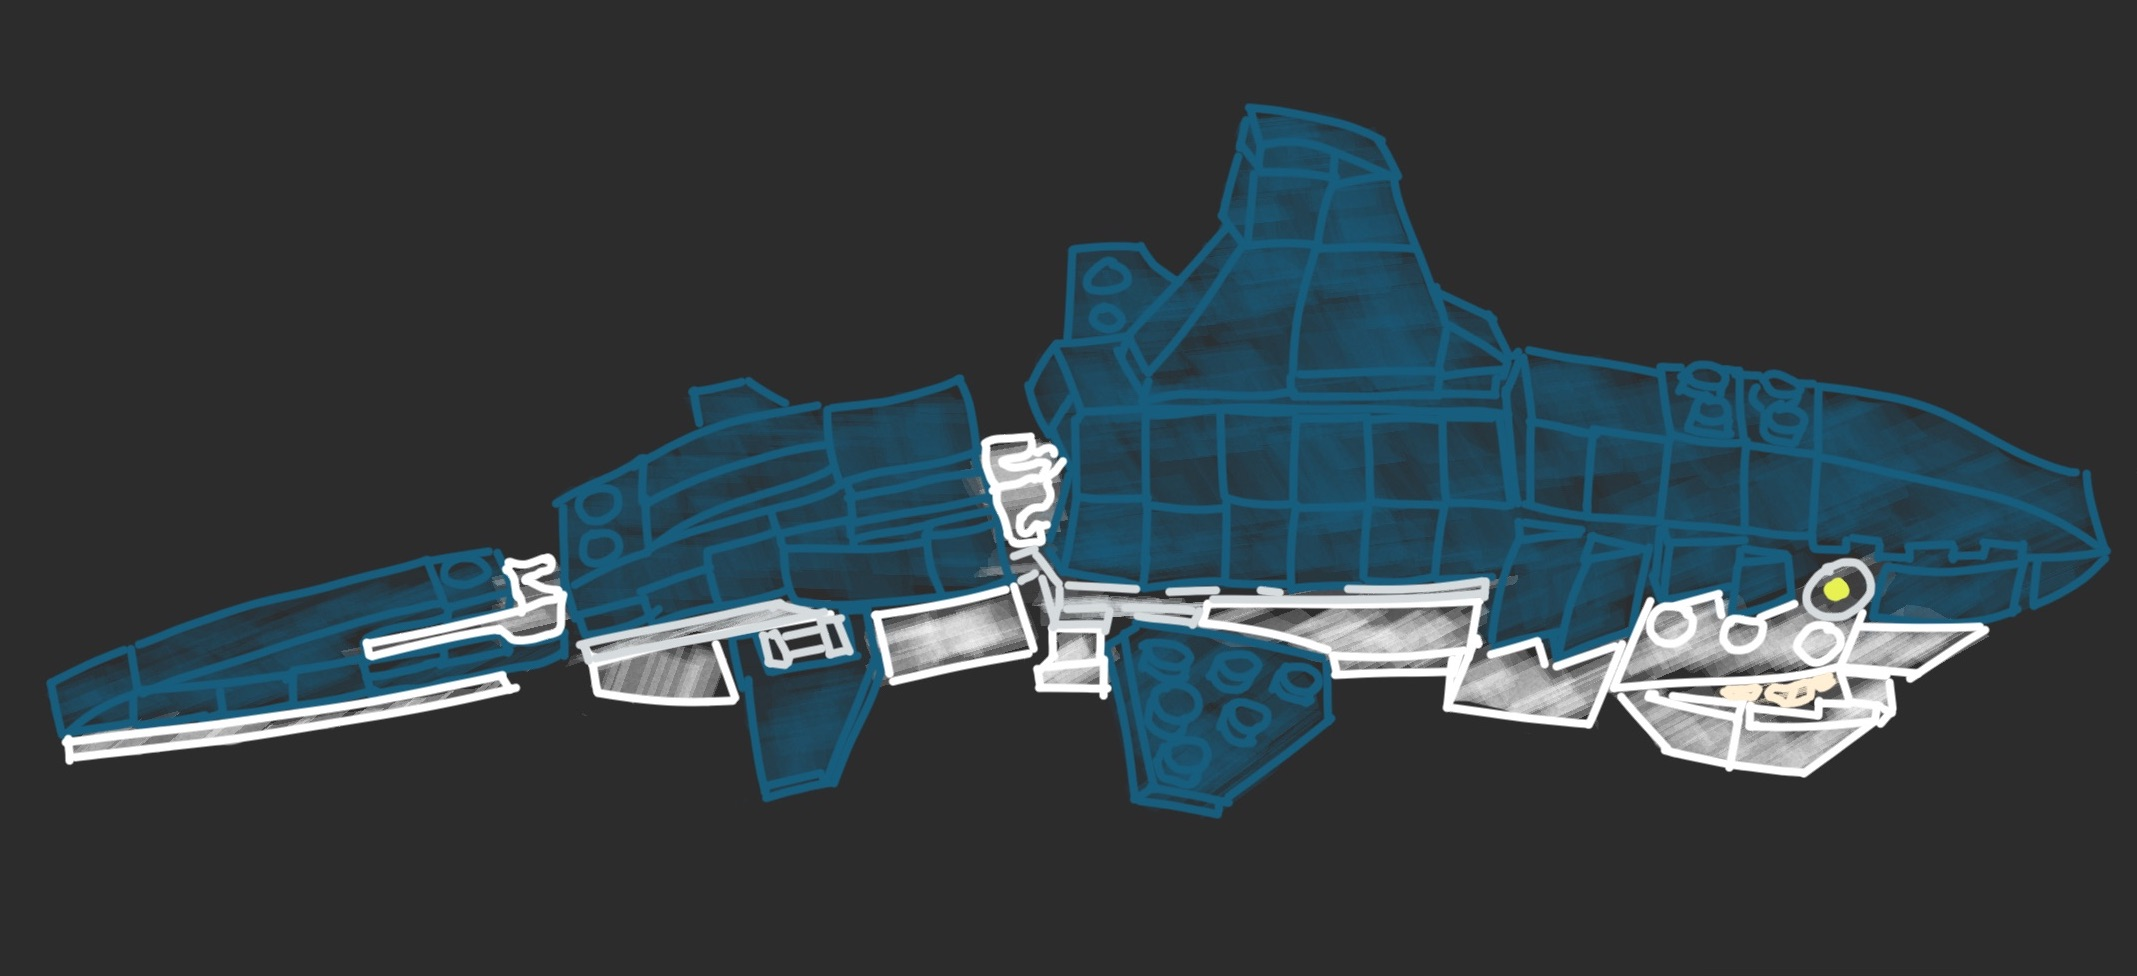
\includegraphics[width=\textwidth]{figures/legoshark} \caption[When simple tools have a common interface that allows them to be combined in different ways, like Legos, they can be combined to create complex structures, like this Lego shark]{When simple tools have a common interface that allows them to be combined in different ways, like Legos, they can be combined to create complex structures, like this Lego shark.}\label{fig:legoshark}
\end{figure}

The tools in the ``tidyverse'' operate on a similar principle. They all input one
of a few very straightforward data types, and they (almost) all output data in
the same format they input it. For most of the tools, their required format for
input and output is the ``tidy data'' format \citep{wickham2014tidy}, called a tidy
\emph{dataframe} in R---this is a dataframe that follows the rules detailed earlier
in this section.

Some of the tools require input and output of \emph{vectors} instead of tidy
dataframes \citep{wickham2014tidy}; a \emph{vector} in R is a one-dimensional string of values,
all of which are of the same data type (e.g., all numbers, or all character
strings, like names). In a tidy dataframe, each column is a vector, and the
dataframe is essentially several vectors of the same length stuck together to
make a table. Having functions that input and output vectors, then, means that
you can use those functions to make changes to the columns in a tidy dataframe.

A few functions in the ``tidyverse'' input a tidy dataframe but output data in a
different format. For example, visualizations are created using a function
called \texttt{ggplot}, as well as its helper functions and extensions. This function
inputs data in a tidy dataframe but outputs it in a type of R object called a
``ggplot object''. This object encodes the plot the code created, so in this case
the fact that the output is in a different format from the endpoint is similar
to with the ``eye'' blocks in Legos, where it's meant as a final output step, and
you don't intend to do anything further in the code once you move into that
step.

This common input / output interface, and the use of small tools that follow
this interface and can be combined in various ways, is what makes the tidyverse
tools so powerful. However, there are other good things about the tidyverse that
make it so popular. One is that it's fairly easy to learn to use the tools, in
comparison to learning how to write code for other R tools \citep{robinson2017teach, peng2018teaching}. The developers who have created the tidyverse tools have
taken a lot of effort to try to make sure that they have a clear and consistent
\emph{user interface} across tools \citep{wickham2017tidy, bryan2017data}. So far, we've
talked about the interface between functions, and how a common \emph{input / output
interface} means the functions can be chained together more easily. But there's
another interface that's important for software tools: the rules for how a
computer users employ that tool, or the \emph{user interface}.

To help understand a user interface, and how having a consistent user interface
across tools is useful, let's think about a different example---cars. When you
drive a car, you get the car to do what you want through the steering wheel, the
gas pedal, the break pedal, and different knobs and buttons on the dashboard.
When the car needs to give you feedback, it uses different gauges on the
dashboard, like the speedometer, as well as warning lights and sounds.
Collectively, these ways of interacting with your car make up the car's \emph{user
interface}. In the same way, each function in a programming language has a
collection of parameters you can set, which let you customize the way the
function runs, as well as a way of providing you output once the function has
finished running and the way to provide any messages or warnings about the
function's run. For functions, the software developer can usually choose design
elements for the function's user interface, including which parameters to
include for the function, what to name those parameters, and how to provide
feedback to the user through messages, warnings, and the final output.

If a collection of tools is similar in its user interfaces, it will make it
easier for users to learn and use any of the tools in that collection once
they've learned how to use one. For cars, this explains how the rental car
business is able to succeed. Even though different car models are very different
in many characteristics---their engines, their colors, their software---they are
very consistent in their user interfaces. Once you've learned how to drive one
car, when you get in a new car, the gas pedal, brake, and steering wheel are
almost guaranteed to be in about the same place and to operate about the same
way as in the car you learned to drive in. The exceptions are rare enough to be
memorable---think how many movies have a laughline from a character trying to
drive a car with the driver side on the right if they're used to the left or
vice versa.

The tidyverse tools are similarly designed so that they all have a very similar
user interface. For example, many of the tidyverse functions use a parameter
named ``.data'' to refer to the tidy dataframe to input into the function, and
this parameter is often the first listed for functions. Similarly, parameters
named ``.vars'' and ``.funs'' are repeatedly used over tidyverse functions, with the
same meaning in each case. What's more, the tidyverse functions are typically given names
that very clearly describe the action that the function does, like \texttt{filter},
\texttt{summarize}, \texttt{mutate}, and \texttt{group}. As a result, the final code is very clear
and can almost be ``read'' as a natural language, rather than code.

\begin{quote}
``Another part of what makes the Tidyverse effective is harder to see and,
indeed, the goal is for it to become invisible: conventions. The Tidyverse
philosophy is to rigorously (and ruthlessly) identify and obey common
conventions. This applies to the objects passed from one function to another
and to the user interface each function presents. Taken in isolation, each
instance of this seems small and unimportant. But collectively, it creates
a cohesive system: having learned one component you are more likely to be
able to guess how another different component works.'' \citep{bryan2017data}
\end{quote}

\begin{quote}
``The goal of {[}the tidy tools{]} principles is to provide a uniform interface so
that tidyverse packages work together naturally, and once you've mastered one,
you have a head start on mastering the others.'' \citep{wickhem2017tidy}
\end{quote}

As a result, the tidyverse collection of tools is pretty easy to learn, compared
to other sets of functions in scripting languages, and pretty easy to expand
your knowledge of once you know some of its functions. Several people who teach
R programming now focus on first teaching the tidyverse, given these
characteristics \citep{robinson2017teach, peng2018teaching}, and it's often a
first focus for online courses and workshops on R programming. Since it's main
data structure is the ``tidy data'' structure, it's often well worth recording
data in this format so that all these tools can easily be used to explore and
model the data.

\begin{quote}
``All our code is underpinned by the principles of tidy data, the
grammar of data manipulation, and the tidyverse R packages developed
by Wickham. This deliberate philosophy for thinking
about data helped bridge our scientific questions with the data processing
required to get there, and the readability and conciseness of
tidyverse operations makes our data analysis read more as a story
arc. Operations require less syntax---which can mean fewer potential
errors that are easier to identify---and they can be chained together,
minimizing intermediate steps and data objects that can cause clutter and
confusion. The tidyverse tools for wrangling data have
expedited our transformation as coders and made R less intimidating to
learn.'' \citep{lowndes2017our}
\end{quote}

\hypertarget{using-tidyverse-tools-with-data-in-the-tidy-data-format}{%
\subsection{Using tidyverse tools with data in the ``tidy data'' format}\label{using-tidyverse-tools-with-data-in-the-tidy-data-format}}

The tidyverse includes tools for many of the tasks you might need to
do while managing and working with experimental data. When you download
R, you get what's called \emph{base R}. This includes the main code that drives
anything you do in R, as well as functions for doing many core tasks.
However, the power of R is that, in addition to base R, you can also add
onto R through what are called \emph{packages} (sometimes also referred to
as \emph{extensions} or \emph{libraries}). These are kind of like ``booster packs''
that add on new functions for R. They can be created and contributed
by anyone, and many are collected through a few key repositories like
CRAN and Bioconductor.

All the tidyverse tools are included in R extension packages, rather than base
R, so once you download R, you'll need to download these packages as well to use
the tidyverse tools. The core tidyverse functions include functions to read in
data (the \texttt{readr} package for reading in plain text, delimited files, \texttt{readxl}
to read in data from Excel spreadsheets), clean or summarize the data (the
\texttt{dplyr} package, which includes functions to merge different datasets, make
new columns as functions of old ones, and summarize columns in the data, either
as a whole or by group), and reformat the data if needed to get it in a tidy
format (the \texttt{tidyr} package). The tidyverse also includes more precise tools,
including tools to parse dates and times (\texttt{lubridate}) and tools to work with
character strings, including using regular expressions as a powerful way to find
and use certain patterns in strings (\texttt{stringr}). Finally, the tidyverse
includes powerful functions for visualizing data, based around the \texttt{ggplot2}
package, which implements a ``grammar of graphics'' within R.

You can install and load any of these tidyverse packages one-by-one using the
\texttt{install.packages} and \texttt{library} functions with the package name from within R.
If you are planning on using many of the tidyverse packages, you can also
install and load many of the tidyverse functions by installing a package called
``tidyverse'', which serves as an umbrella for many of the tidyverse packages.

In addition to the original tools in the tidyverse, many people have developed
\emph{tidyverse} extensions---R packages that build off the tools and principles in
the tidyverse. These often bring the tidyverse conventions into tools for
specific areas of science. For example, the \texttt{tidytext} package provides tools to
analyze large datasets of text, including books or collections of tweets, using
the tidy data format and tidyverse-style tools. Similar tidyverse extensions
exist for working with network data (\texttt{tidygraph}) or geospatial data (\texttt{sf}).
Extensions also exist for the visualization branch of the tidyverse
specifically. These include \emph{ggplot extensions} that allow users to create
things like calendar plots (\texttt{sugrrants}), gene arrow maps (\texttt{gggene}), network
plots (\texttt{igraph}), phytogenetic trees (\texttt{ggtree}) and anatogram images
(\texttt{gganatogram}). These extensions all allow users to work with data that's in a
``tidy data'' format, and they all provide similar user interfaces, making it
easier to learn a large set of tools to do a range of data analysis and
visualization, compared to if the set of tools lacked this coherence.

\hypertarget{practice-quiz}{%
\subsection{Practice quiz}\label{practice-quiz}}

\hypertarget{designing-templates-for-tidy-data-collection}{%
\section{Designing templates for ``tidy'' data collection}\label{designing-templates-for-tidy-data-collection}}

This module will move from the principles of the ``tidy'' data format to the
practical details of designing a ``tidy'' data format to use when collecting
experimental data. We will describe common issues that prevent biomedical
research datasets from being ``tidy'' and show how these issues can be avoided. We
will also provide rubrics and a checklist to help determine if a data collection
template complies with a ``tidy'' format.

\textbf{Objectives.} After this module, the trainee will be able to:

\begin{itemize}
\tightlist
\item
  Identify characteristics that keep a dataset from being `tidy'
\item
  Convert data from an ``untidy'' to a ``tidy'' format
\end{itemize}

It is usually very little work to record data in a structure
that follows the ``tidy data'' principles, especially if you are planning to record
the data in a two-dimensional, tabular format already, and following these
principles can bring some big advantages. We explain these rules and provide
examples of biomedical datasets that both comply and don't comply with these
principles, to help make it clearer how you could structure a ``tidy-compliant''
structure for recording experimental data for your own research.

If the data is the same regardless of whether it's ``tidy'' or not, then why all
the fuss about following the ``tidy'' principles when you're designing the format
you'll use to record your data? The magic here ix this---if you follow these
principles, then your data can be immediately input into a collection of
powerful tools for visualizing and analyzing the data, without further cleaning
steps (as discussed in the previous module). What's more, all those tools (the
set of tools is calld the ``tidyverse'') will typically \emph{output} your data in a
``tidy'' format, as well.

Once you have tools that input and output data in the same way, it becomes very
easy to model each of the tools as ``small, sharp tools''---each one does one
thing, and does it really well. That's because, if each tool needs the same
type of input and creates that same type of output, those tools can be chained
together to solve complex problems. The alternative is to create large software
tools, ones that do a lot to the input data before giving you some output.
``Big'' tools are harder to understand, and more importantly, they make it hard
to adapt your own solutions, and to go beyond the analysis or visualization that
the original tool creators were thinking of when they created it. Think of it this
way---if you were writing an essay, how much more can you say when you can mix and
match words to create your own sentences versus if you were made to combine
pre-set sentences?

\hypertarget{creating-the-rules-for-collecting-data-in-the-same-time-each-time}{%
\subsection{Creating the rules for collecting data in the same time each time}\label{creating-the-rules-for-collecting-data-in-the-same-time-each-time}}

It is likely that there are certain types of experiments that you conduct
regularly, and that they're often trying to answer the same type of
question and generate data of a consistent type and structure. This is
a perfect chance to lay down rules or a pattern for how members of
your research group will record that data.

These rules can include:

\begin{enumerate}
\def\labelenumi{\arabic{enumi}.}
\tightlist
\item
  How many units of observation does the experiment typically have?
  Say, for example, that you are measuring the influence of two drugs on
  bactieral load in an animal at
  three time points. There may be some measurements taken at the unit of the drug
  (for example, measurements related to its chemical composition) and some
  taken at the unit of animal and time point (for example, the concentration of drug in
  an animal's blood at a certain time point). This will help you define how many
  tables you should use to collect the data---one for each unit of observation.
\item
  Which measurements will be recorded for each observation? In tidy data, the measurements
  taken for an observation are recorded in rows, so you then specify what
  column names should be used for each measurement (e.g., ``sample\_time'',
  ``animal\_weight''). If data is being recorded using multiple tables (because there
  are multiple units of observation), make sure that each table include
  ``ID'' columns that can be used to link across the tables. For example, each
  table might have a column with a unique ID for each drug being tests, or tables
  with measurements on animals might each have a column that uniquely identifies
  the animal in an observation.
\item
  What units will be used for recording each measurement? For timestamp-type
  measurments, like the date and time that an experiment started and the time of
  each sample measurement, what timezone will be used? (Even if it's always the
  same one, this can come in useful every now and then if you need to figure out
  something like whether that location's timezone followed Daylight Savings Time,
  for an experiment that spans the switch between Standard and Daylight Savings).
\end{enumerate}

{[}Figure: Three tables---measurements on a drug (chemistry), measurements on an animal (weight),
measurements on an animal at time points (drug concentration){]}

You can then take this information and design a \emph{template} for collecting that
type of data. A template is, in this case, a file that gives the ``skeleton'' of
the table or tables. You will create this template file and save it somewhere
easy for lab members to access, with a filename that makes it clear that this is
a template. For example, you may create a folder with all the templates for
tables for your experiment, and name a template in it for collecting something
like animal weights at the start of the experiment something like
``animal\_wt\_table\_template.csv'' or ``animal\_wt\_table\_template.xlsx''.
Each time someone starts an experiment collecting that type of data, he or she
can copy that template file, move it to the directory with files for that
experiment and rename it. When you open that copy of the file, you can record
observations directly into it.

{[}Figure: Example template file{]}

\begin{verbatim}
####################################################################################
####################################################################################
#
# Column names and meanings
#
# animal_id:        A unique identifier for each animal. 
# animal_wt_g:      The weight of the animal, recorded in grams. 
# date_wt_measured: The date that the animal's weight was measured, recorded as 
#                   "month day, year", e.g., "Jan 1, 2019"
# cage_id:          A unique identifier for the case in which the animal was housed
# 
# Other table templates for this experiment type: 
# drug_conc_by_time.csv: A template for recording drug concentrations in the animals
#                        by time point
# 
animal_id, animal_wt_g, date_wt_measured, cage_id
   "A101",        50.2,   "Jan 1, 2019",      "B"    
\end{verbatim}

Adding in one row of sample values, to be deleted each time the template is
copied and used, can be a very helpful addition. This will help the user remember
the formats that are expected for each column (for example, the format the
date should be recorded in), as well as small details like which columns should
include quotation marks.

These template tables can be created as flat files, like comma-separated value
files. However, if this is too big of a jump, they can also be created as
spreadsheet files. Many of the downsides of spreadsheet files are linked to
the use of embedded macros, integration of raw and processed / calculated data,
and other factors, rather than related to their use as a method to record data.
However, do note that plain text files like flat files can be opened in RStudio
in a spreadsheet-like view in RStudio. Data can be recorded directly here, in
a format that will feel comfortable for spreadsheet users, but without all the
bells and whistles that we're aiming to avoid in spreadsheet programs like Excel.

{[}Figure---Opening a csv file with a spreadsheet like view{]}

There are some advantages to shifting to record data in flat files like CSVs,
rather than Excel files, and using the spreadsheet-style view in RStudio to work
with those files if you find it easier than working with the files in a text
editor (which can get tough, since the values in a column don't always visually
line up, and you have to remember to put in the right number of columns). By
recording the data in a plain text file, you can later move to tracking changes
that are made to the data using the version control tool \emph{git}. This is a
powerful tool that can show who made changes to a file and when, with exact
details on the changes made and room for comments on why the change was made.
However, \emph{git} does not provide useful views of changes made to binary files
(like Excel), only those made in plain text files. Further, plain text files are
guaranteed to not try to ``outsmart'' you---for example, they will not try to
convert something that looks like a date into a date. Instead, they will leave
things exactly as you typed them in. Finally, later in this book we will build
up to creating templates that do even more---for example, templates for reports
you need to write and presentations you need to give, as well as templates for
the whole structure of a project. Plain text files fit very nicely into this
developing framework, while files in complex binary formats like xlxs don't fit
as naturally.

Google Sheets is another tool that might come in useful. {[}More about using this
with R.{]}

This idea of creating template files for data recording isn't
revolutionary---many laboratory groups have developed spreadsheet template files
that they share and copy to use across similar experiments that they conduct.
The difference here is in creating a table for recording data \emph{that follows the
tidy data principles}, or at least comes close to them (any steps away from
characteristics like embedded macros and use of color to record information will
be helpful).

The next chapter will walk through two examples of changing from non-tidy table
templates to ones that record data in a way that follows the tidy data
principles.

\hypertarget{subsection-1}{%
\subsection{Subsection 1}\label{subsection-1}}

\begin{quote}
``Or maybe your goal is that your data is \emph{usable} in a wide range of
applications? If so, consider adopting standard formats and metadata
standards early on. At the very least, keep track of versions of data
and code, with associated dates.'' \citep{goodman2014ten}
\end{quote}

\begin{quote}
``Standards for data include, for example, data formats, data exchange
protocols, and meta-data controlled vocabularies.'' \citep{barga2011bioinformatics}
\end{quote}

\begin{quote}
``Software systems are transparent when they don't have murky corners or hidden
depths. Transparency is a passive quality. A program is passive when it is possible
to form a simple mental model of its behavior that is actuaally predictive for all
or most cases, because you can see through the machinery to what is actually going
on.'' \citep{raymond2003art}
\end{quote}

\begin{quote}
``Software systems are discoverable when they include features that are designed
to help you build in your mind a correct mental model of what they do and how they
work. So, for example, good documentation helps discoverability to a programmer. Discoverability
is an active quality. To achieve it in your software, you cannot merely fail to be obscure,
you have to go out of your way to be helpful.'' \citep{raymond2003art}
\end{quote}

\begin{quote}
``Elegant code does much with little. Elegant code is not only correct but visibly,
\emph{transparently} correct. It does not merely communicate an algorithm to a computer,
but also conveys insight and assurance to the mind of a human that reads it. By seeking
elegance in our code, we build better code. Learning to write transparent code is a first,
long step toward learning how to write elegant code---and taking care to make code
discoverable helps us learn how to make it transparent. Elegant code is both transparent and
discoverable.'' \citep{raymond2003art}
\end{quote}

\begin{quote}
``To design for transparency and discoverability, you need to apply every tactic for
keeping your code simple, and also concentrate on the ways in which your code is a
communication to other human beings. The first questions to ask, after `Will this design
work?' are `Will it be reaadable to other people? Is it elegant?' We hope it is clear \ldots{}
that these questions are not fluff and that elegance is not a luxury. These qualities
in the human reaction to software are essential for reducing its bugginess and
increasing its long-term maintainability.'' \citep{raymond2003art}
\end{quote}

\begin{quote}
``Software is maintainable to the extent that people who are not its author can
successfully understand and modify it. Maintainability demands more than code that
works; it demands code that follows the Rule of Clarity and communicates successfully
to human beings as well as the computer.'' \citep{raymond2003art}
\end{quote}

\hypertarget{dont-repeat-yourself}{%
\subsection{Don't Repeat Yourself!}\label{dont-repeat-yourself}}

One of the core tenets of programming is the philosophy of ``Don't Repeat
Yourself'' (a.k.a., the ``DRY Principle'').{[}Source of ``Don't Repeat
Yourself''---\emph{The Pragmatic Programmer}{]} With programming, you can invest a
little bit of time to code your computer to do things that take a lot of your
time otherwise. In this way, you can automate repetitive tasks.

\begin{quote}
``The DRY principle, for Don't Repeat Yourself, is one of the colloquial tenets
of programming. That is, you should name things once, do things once, create a
function once, and let the computer repeat itself.'' {[}ford2015code{]}
\end{quote}

\begin{quote}
``Code, in other words, is really good at making things \emph{scale}. Computers
may require utterly precise instructions, but if you get the instructions
right, the machine will tirelessly do what you command over and over and
over again, for users around the world. \ldots{} Solve a problem once, and you've
solved it for everyone.'' {[}Coders, p.~20{]}
\end{quote}

\begin{quote}
``Since they have, at their beck and call, machines that can repeat
instructions with robotic perfection, coders take a dim view of doing
things repetitively themselves. They have a dislike of inefficiency
that is almost aesthetic---they recoil from it as if from a disgusting
smell. Any opportunity they have to automate a process, to do something
more efficiently, they will.'' {[}Coders, p.~20{]}
\end{quote}

\begin{quote}
``Programmers are obsessed with efficiency. \ldots{} Removing the friction
from a system is an aesthetic joy; {[}programmers'{]} eyes blaze when they
talk about making something run faster, or how they eliminated some
bothersome human effort from a process.'' {[}Coders, p.~122{]}
\end{quote}

\begin{quote}
``Computers, in many ways, inspire dreams of efficiency greater than
any tool that came before. That's because they're remarkably good at
automating repetitive tasks. Write a script once, set it running, and
the computer will tirelessly execute it until it dies or the power
runs out. What's more, computers are strong in precisely the ways that
humans are weak. Give us a repetitive task, and our mind tends to
wander, so we gradually perform it more and more irregularly. Ask us
to do something at a precise time or interval, and we space out and
forget to do it. \ldots{} In contrast, computers are clock driven and superb
at doing the same thing at the same time, day in and day out.''
{[}Coders, p.~124{]}
\end{quote}

\begin{quote}
``Larry Wall, the famous coder and linguist who created the Perl
programming language, deeply intuited this coderly aversion to
repetition. In his book on Perl, he and coauthors wrote that one of the
key virtues of a programmer is `laziness'. It's not that you're too lazy
for coding. It's that you're too lazy to do routine things, so it
inspires you to automate them.'' {[}Coders p.~126{]}
\end{quote}

In scientific research, there are a lot of these repetitive tasks, and as tools for
automation continue to develop, there are many opportunities to ``automate away'' busywork.

\begin{quote}
``Science often involves repetition of computational tasks such as processing
large number of data files in the same way or regenerating figures each time
new data are added to an existing analysis. Computers were invented to do these
kinds of repetitive tasks but, even today, many scientists type the same
commands in over and over again or click the same buttons repeatedly.'' {[}wilson2014best{]}
\end{quote}

\begin{quote}
``Whenever possible, rely on the execution of programs instead of manual procedures
to modify data. Such manual procedures are not only inefficient and error-prone,
they are also difficult to reproduce.'' {[}sandve2013ten{]}
\end{quote}

\begin{quote}
``Other manual operations like the use of copy and paste between documents should
also be avoided. If manual operations cannot be avoided, you should as a minimum
note down which data fiels were modified or moved, and for what purpose.'' {[}sandve2013ten{]}
\end{quote}

Statisticians have been doing this for a while for data cleaning analysis tasks.
For example, if you need to read in an Excel file into a statistical programming
language like R, you could write a few lines of code to do that anew each time
you get a new file. However, say you get Excel files over and over that follow
the same format--for example, files with the same number of columns, the same
names for those columns, and the same type of data. You can write a \emph{script}---a
recorded file with a few lines of code, in this case---that reads in the file.
You can apply this script to each new file.

This saves you a little bit of time. It also ensures that you do the exact same thing
with every file you get. It also means that you can reproduce what you do now to a file
in the future. Say, for example, that you are working on a project and you read in a file
and conduct an analysis. Your laboratory group sends the paper out for review. Months
later, you get back comments from the reviewers, and they are wondering what would
happen if you had analyzed the data a bit differently---say, used a different
statistical test. If you use a script to read in the data file, then when you re-run
it to address the reviewers' comments, you can be sure that you are getting your
data into the statistical program in the exact same way you did months ago, and so
you're not unintentionally introducing differences in your results because you
are doing some small things differently in processing the file.

This idea can extend across the full data analysis you do on a project. You are only
saving a little bit of time and effort, maybe, by automating the step where you read
the data from a spreadsheet into the statistical program. And it takes some time to
write that script the first time, so it can be tempting to do it fresh each time you
need to do it. However, you can also write scripts that will automate cleaning your data.
Maybe you want to identify data points with very high (maybe suspect) values for a certain
measurement, or remove observations with missing data. You can also write scripts that
will automating processing your data---doing things like calculating the time since the
start of an experiment based on the recorded sampling time for an observation. Each of
these steps might be small, but the time saved really adds up since you typically
need to perform many of these steps each time you run a new experiment.

There are many cases in life where you'll need to make the choice between spending
some time upfront to make something more efficient, versus doing it more quickly the first
time but then having to do it ``from scratch'' again each following time. For example,
say that you're teaching a class, and you need to take attendance for each class period.
You could write down the names of each student at the first class and save that, and
then the next class write down the name of each student who shows up that day on a separate
sheet of paper, and so on for each class meeting. Conversely, you could take some extra
time before the first class and create a table or spreadsheet file with every student's
name and the date of each class, and then use that to mark attendance. The first method
will be quicker the first day, but more time consuming each following time. The second
method requires a small initial investment, but with time-saving returns in the following
class meetings.

For people who use scripts and computer programs to automate their data-related tasks,
it quickly becomes very confusing how anyone who doesn't could argue that they don't because
they don't have time to learn how to. The amount of time you end up saving based on your
initial investment is just so high if you're working with data, that it would have to take
a huge time investment to not be worth it. Plus---the thrill of running something that you've
automated! It's a very similar feeling to the feeling you get when a student or postdoc that
you've spent a lot of time training has gotten to the point where you can just ask them
to run something, and they do, and it means you don't have to.

Here are some of the problems that are solved by automating your small tasks:

\begin{enumerate}
\def\labelenumi{\arabic{enumi}.}
\item
  \textbf{It gets done the same way every single time.} Even simple tasks can be done with
  numerous small modifications. You will probably remember some of those choices and
  settings and modifications the next time you need to do the same thing, but probably
  not all of them, and so those choices will not be exact from one time to the next.
  If the computer is doing it based on a clear set of instructions, it will be.
\item
  \textbf{It gets done more quickly.} Or if not more quickly (some large data might take
  some time to process), at least the spent time is the computers time, not yours. You
  can leave the computer to run the script while you get on with other things that
  a computer can't do.
\item
  \textbf{Anyone who does it can do it the same way.} Just as you might not do something
  exactly the same way from one time to the next, one person in a laboratory group is
  likely to do things at least slightly different than other members of the group.
  Even with very detailed instructions, few instructions written for humans can be
  so detailed and precise to ensure that something is done exactly the same way by
  everyone who follows them. If everyone is given the same computer script to run,
  however, and they all instruct the computer to run that script, the task will be
  done in exactly the same way.
\item
  \textbf{It is easier teach new people how to do the task.} Often, with a script to
  automate a task, you just need to teach someone new to the laboratory group how
  to get the computer to run a script in a certain language. When you need them to
  run a new script, the process will be the same. The script encapsulates all the
  task-specific details, and so the user doesn't need to understand all of them to
  get something to run. What's more, once you want to teach a new lab member how
  everything it working, so they can understand the full process, the script provides
  the exact recipe. You can teach them how to read and understand scripts in that
  language, and then the scripts you've created to automate tasks serve as a recipe
  book for everything going on in terms of data analysis for the lab.
\item
  \textbf{You can create tools to share with others.} If you've written a script that's
  very useful, with a bit more work you can create it into a tool that you can share
  with other research groups and perhaps publish a paper about. Papers about R
  software extensions (also called \emph{packages}) and data analysis workflows and
  pipelines are becoming more and more common in biological contexts.
\item
  \textbf{It's more likely to be done correctly.} Boring, repetative tasks are easy
  to mess up. We get so bored with them, that we shift our brains into a less-attentive
  gear when we're working on them. This can lead to small, stupid mistakes, ones
  at the level of typos but that, with data cleaning and analysis, can have much
  more serious ramifications.
\end{enumerate}

\begin{quote}
``We view workflows as a paradigm to: 1) expose non-experts to well-understood
end-to-end data analysis processes that have proven successful in challenging
domains and represent the state-of-the-art, and 2) allow non-experts to easily
experiment with different combinations of data analysis processes, represented
as workflows of computations that they can easily reconfigure and that the
underlying system can easily manage and execute.'' {[}hauder2011making{]}
\end{quote}

\begin{quote}
``While reuse {[}of workflows{]} by other expert scientists saves them time and
effort, reuse by non-experts is an enabling matter as in practice they would
not be able to carry out the analytical tasks without the help of
workflows.'' {[}hauder2011making{]}
\end{quote}

\begin{quote}
``We observed that often steps that could be easily automated were performed manually
in an error-prone fashion.'' {[}vidger2008supporting{]}
\end{quote}

Biological research is quickly moving where a field where projects often required
only simple and straightforward data analysis once the experimental data was
collected---with the raw data often published directly in a table in the manuscript---to
a field with very complex and lengthy data analysis pipelines between the experiment
and the final manuscript. To ensure rigor and clarity in the final research results,
as well as to allow others to reproduce the results exactly, the researcher must
document all details of the computational data analysis, and this is often
missing from papers. RMarkdown documents (and their analogues) can provide all these
details unambiguously---with RMarkdown documents, you can even run a command to
pull out all the code used within the document, if you'd like to submit that
code script as a stand-alone document as a supplement to a manuscript.

\begin{quote}
``More recently, scientists who are not themselves computational experts are
conducting data analysis with a wide range of modular software tools and packages.
Users may often combine these tools in unusual or nove ways. In biology,
scientists are now routinely able to acquire and explore data sets far beyond
the scope of manual analysis, including billions of DNA bases, millions of genotypes,
and hundreds of thousands of RNA measurements. \ldots{} While propelling enormous
progress, this increasing and sometimes `indirect' use of computation poses
new challenges for scientific publication and replication. Large datasets are
often analyzed many times, with modifications to the methods and parameters, and
sometimes even updates of the data, until the final results are produced. The
resulting publication often gives only scant attendtion to the computations details.
Some papers have suggested these papers are `merely the advertisement of
scholarship whereas computer programs, input data, parameter values, etc., embody
the scholarship itself.' However, the actual code or software `mashup' that
gave rise to the final analysis may be lost or unrecoverable.'' {[}mesirov2010accessible{]}
\end{quote}

\begin{quote}
``Bioinformatic analyses invariably involve shepherding files through a series
of transformations, called a pipeline or workflow. Typically, these transformations
are done by third-part executable command line software written for Unix-compatible
operating systems. The advent of next-generation sequencing (NGS), in which millions
of short DNA sequences are used as the source input for interpreting a range of
biological phenomena, has intensified the need for robust pipelines. NGS analyses
tend to involve steps such as sequence alignment and genomic annotation that are
both time-intensive and parameter-heavy.'' {[}leipzig2017review{]}
\end{quote}

\begin{quote}
``\textbf{Rule 7: Always Store Raw Data behind Plots.} From the time a figure is first
generated to it being part of a published article, it is often modified several
times. In some cases, such modifications are merely visual adjustments to
improve readability, or to ensure visual consistency between figures. If raw data
behind figures are stored in a systematic manner, so as to allow raw data for
a given figure to be easily retrieved, one can simply modify the plotting
procedure, instead of having to redo the whole analysis. An additional
advantage of this is that if one really wants to read fine values in a figure,
one can consult the raw numbers. \ldots{} When plotting is performed using a
command-based system like R, it is convenient to also store the code
used to make the plot. One can then apply slight modifications to these
commands, instead of having to specify the plot from scratch.'' {[}sandve2013ten{]}
\end{quote}

\hypertarget{dont-repeat-your-report-writing}{%
\subsection{Don't repeat your report-writing!}\label{dont-repeat-your-report-writing}}

Until a few years ago, statisticians and data analysts frequently automated the
data cleaning, processing, and analysis tasks. But that still left the paper
and report writing to be done by hand. This process is often repetitive. You would
do your analysis and create some tables or figures. You would save these from
your statistical program and then paste them into your report or paper draft.
If you decided that you needed to change your analysis a bit, or if you got a new
set of data to analyze in a similar way, you had to go back to the statistical
program, run things again there, save the tables and figure files again, and paste
them in the report or paper again to replace the outdated version. If there were
numbers from the analysis in the text of the paper, then you had to go back through
the text and update all of those with the newer numbers, too.

Do you still write your papers and reports like this? I can tell you that there is
now a \emph{much} better way. Computer scientists and other programmers started thinking
quite a while ago about how to create documents that combine computer code and
text for humans, and to do it in a way where the computer code isn't just a static
copy of what someone once told the computer to do, but instead a living, working,
\emph{executable} set of instructions that the computer can run anytime you ask it to.

These ideas first perculated with Donald Knuth, who many consider to be the greatest
computer programmer of all time {[}Bill Gates, for example, has told anyone who reads Dr.~Knuth's
magnum opus, \emph{The Art of Computer Programming}, to come see him right away about a job{]}.
As Dr.~Knuth was writing a book on computer programming, he became frustrated with the
quality of the typesetting used in the final book. In a field that requires a lot of mathematical
and other symbols incorporated into the text, it takes a bit more to make an attractive
book than with simpler text. Dr.~Knuth therefore took some time to create a programming
for typesetting. (You may have heard of it---if you ever notice that a journal's
Instructions to Authors allow authors to submit articles in ``LaTeX'' or ``TeX'', that's
using a system built off of Donald Knuth's typesetting program.)

And \emph{then}, once he had that typesetting program, he started thinking about how
programmers document their code. When one person does a very small code project,
and that one person is the only person who will ever go back to try to modify or
understand the code, that person might be able to get away with poor
documentation in the code. However, interesting code projects can become
enormous, with many collaborators, and it becomes impossible to understand and
improve the code if it doesn't include documentation explaining, in human terms,
what the code is doing at each step, as well as some overall documentation
explaining how different pieces of the code coordinate to get something big
done.

Traditionally, code was documented by including small comments within the code. These comments
are located near the code that they explain, and the order of the information in the
code files are therefore dominated by the order of the instructions to the computer,
not the order that you might explain what's going on to a human. To ``read'' the code and
the documentation, you end up hopscotching through the code, following the code inside
one function when it calls another function, for example, to where the code for that
second function is defined and then back to the first, and so on. You often follow paths as
you get deeper and deeper into helper functions and the helper functions for those functions,
that you feel like you're searching through a set of Russian dolls and then coming back up
to start on a new set of Russian dolls later down the line.

Donald Knuth realized that, with a good typesetting program that could itself be programmed,
you could write your code so that the documentation for humans took precedence, and could
be presented in a very clear and attractive final document, rather than hard-to-read
computer code with some plain-text comments sprinkled in. Computers don't care what order
the code is recorded in---as long as you give them some instructions on how to decipher
code in a certain format or order, they can figure out how to use it fine. But human brains
are a bit more finicky, and we need clear communication, laid out in a logical and helpful
order. Donald Knuth created a paradigm of \emph{literate programming} that interleaved
executable code inside explanations written for humans; by making the code executable, it
meant that the document was a living guide. When someone changed the program, they did
it by changing the documentation---documentation wasn't left as the final, often neglected,
step to refine once the ``real code'' was written (and the ``real work'' done).

\begin{quote}
``Programs must be written for people to read, and only incidentally for machines
to execute. A great program is a letter from current you to future you or
the the person who inherits your code. A generous humanistic document.'' {[}ford2015what{]}
\end{quote}

Well, this was a fantastic idea. It hasn't been universely leveraged, but the projects that
do leverage it are much stronger for it. But that's not where the story ends. If you are
someone who does a little bit of coding (maybe small scripts to analyze and visualize your
data, for example) and a lot of ``documenting'' of the results, and if you're not planning
on doing a lot of large coding projects or creating software tools, it's not immediately
how you'd use these literate programming ideas.

Well, there are many people who do a little bit of programming in service to a larger
research project. While they are not creating software that needs classical software
documentation, they do want to document the results that they get when they run their
scripts, and they want to create reports and journal articles to share what they've
found. Several people took the ideas behind literate programming---as it's used to
document large software projects---and leveraged it to create tools to automate
writing in data-related fields.

{[}F. Leisch?{]} was the first to do this with the R programming language, with a
tool called ``Sweave'' (``S''-``weave'', as R builds off of another programming
language called ``S'' and Leisch's program would ``weave'' together S / R code and
writing). This used Donald Knuth's typesetting program. It allowed you to write
a document for humans (like a report or journal article) and to intersperse bits
of code in the paper. You'd put each code piece in the spot in the paper where
the text described what was going on or where you wanted the results that it
generated for example, if you had a section in the Methods where you talked
about removing observations that were outliers, you would add in the code that
took out those outliers right there in the paper. And if you had a placed in the
Results that talked about how your data were different between two experimental
groups, you would add the code that generated the plot to show that right there
in the paper.

To tell the computer how to tell between code and writing, you would add a little
weird combination of text each time that you wanted to ``switch'' into code and then
another one each time you wanted to switch back into writing for humans. (These
combinations were so weird because that guaranteed that it was a combination you
would probably never want to type otherwise, so you wouldn't have a lot of
cases of the computer getting confused between whether the combo meant to switch
to code or whether it was just something that came up in the regular writing.)
You'd send the document, code and writing and all, through R once you had it
written up. R would ignore everything that wasn't code. When it got to the code
pieces, it would run them, and if the code created output (like a figure or table),
it would ``write'' that into the document at that point in the text. Then you'd run
the document through Donald Knuth's typesetting program (or an extension of it),
and the whole document would get typeset into an attractive final product (often
a pdf, although you had some choices on the type of output).

This meant that you got very attractive final documents. It also meant that your
data analysis code was well documented---it was ``documented'' by the very article
or report you wrote based on it, because the code was embedded right there in the
final product! It also meant that you could save a lot of time if you needed to
go back and change some of your code later (or input a different or modified dataset).
You just had to change that small piece of code or data input, and then essentially
press a button to put everything together again, and the computer would re-write the
whole report for you, with every figure and table updated. It even let you write
small bits of computer code directly into the written text, in case you need to
write something like ``this study included 52 subjects'', where the ``52'' came from
you counting up the number of rows in one of your datasets---if you later added three
more subjects and re-ran the analysis with the updated dataset, the report would
automatically change to read ``this study included 55 subjects''.

Leisch's system is still out there, but another has been adopted much more
widely, building on it. Yihui Xie started work on a program that tweaked and
improved Leisch's Sweave program, creating something called ``knitr''
(``knit''-``R''---are you noticing a pattern in the names?). Xie's knitr program,
along with its extensions, is now widely used for data analysis projects. What's
more, it's grown to allow for larger or more diverse writing projects---this
book, for example, is written using an extension called ``bookdown'', and
extensions also exist for create blogs that include executable R code
(``blogdown'') and websites with documentation for R packages (``packagedown'').

So now, let's put these two pieces together. We know that programmers love to
automate small tasks, and we know that there are tools that can be used to
``program'' tasks that involve writing and reporting. So what does this mean if
you frequently need to write reports that follow a similar pattern and start
from similar types of data? If you are thinking like a code, it means that
you can move towards automating the writing of those reports.

One of us was once talking to someone who works in a data analysis-heavy field,
and she was talking about how much time she spends copying the figures that her
team creates, based on a similar analysis of new data that's regularly
generated, into PowerPoint presentations. So, for this weeks report, she's
creating a presentation that shows the same analysis she showed last week, just
with newer data. Cutting and pasting is an enormous waste of time---there are
tools to automate this.

\hypertarget{automating-reports}{%
\subsection{Automating reports}\label{automating-reports}}

First---think through the types of written reports or presentations you've
created in the past year or two. Are there any that follow a similar pattern?
Any that input the same types of data, but from different experiments, and then
report the same types of statistics or plots for them? Are there Excel
spreadsheets your lab uses that generate specific tables or plots that you often
cut and paste for reports or presentations? Look through your computer file
folders or email attachments if you need to---many of these might be small
regular reports that are so regular that they don't pop right to mind. If you
are creating documents that match any of these conditions, you probably have
something ripe for converting to a reusable, automatable template.

\begin{quote}
``Think like Henry Ford; he saw that building cars was a repeatable process and
came up with the moving assembly line method, revolutionizing production. You
may not be building a physical product, but chances are you are producing something.
\ldots{} Look for the steps that are nearly identical each time, so you can build your
own assembly line.'' {[}rose2018dont{]}
\end{quote}

\ldots{} {[}Creating a framework for the report{]}

\begin{quote}
``Odds are, if you're doing any kind of programming, especially Web programming,
you've adopted a framework. Whereas an SDK is an expression of a corporate
philosophy, a framework is more like a product pitch. Want to save time? Tired
of writing old code? Curious about the next new thing? You use a graphics
framework to build graphical applications, a Web framework to build Web
applications, a network framework to build network servers. There are
hundreds of frameworks out there; just about every language has one.
A popular Web framework is Django, which is used for coding in Python.
Instagram was bootstrapped on it. When you sit down for the first time
with Django, you run the command `startproject', and it makes a directory
with some files and configuration inside. This is your project directory. Now
you have access to libraries and services that add to and enhance the standard
library.'' {[}ford2015what{]}
\end{quote}

One key advantage of creating a report template is that it optimizes the time of
statistical collaborators. It is reasonable for a scientists with a couple of
courses worth of statistical training to design and choose the statistical tools
for simple and straightforward data analysis. However, especially as the
biological data collected in experiments expands in complexity and size, a
statistician can recommend techniques and approaches to draw more knowledge
from the data and to appropriately handle non-standard features of the data.
There is substantial work involved in the design of any data analysis pipeline
that goes beyond the very basics. It waste time and resources to recreate this
with each new project, time that---in the case of statistical collaborators---could
probably be better spent in extending data analysis goals beyond the simplest
possible analysis to explore new hypotheses or to add exploratory analysis that
could inform the design of future experiments.

\begin{quote}
``Workflows effectively capture valuable expertise, as they represent how an
expert has designed computational steps and combined them into an
end-to-end process.'' {[}hauder2011making{]}
\end{quote}

When collaborative work between scientists and statisticians can move towards
developing repeatable data analysis scripts and report templates, you will start
to think more about common patterns and common questions that you ask across
many experiments in your research program, rather than focusing on the immediate
needs for a specific project. You can start to think of the data analysis tools
that are general purpose for your research lab, develop those into clean,
well-running scripts or functions, and then start thinking about more
sophisticated questions you want to ask of your data. The statisticians you
collaborate will be able to see patterns across your work and help to develop
global, and perhaps novel, methods to apply within your research program, rather
than piecemeal small solutions to small problems.

\begin{quote}
``Although foundational knowledge is taught in major universities and colleges,
advanced data analytics can only be acquired through hands-on practical training.
Only exposure to real-world datasets allows students to learn the importance of
preparing and cleansing the data, designing appropriate features, and
formulating the data mining task so that the data reveals phenomena of interest.
However, the effort required to implement such complex multi-step data analysis
systems and experiment with the tradeoffs of different algorithms and feature
choices is daunting. For most practical domains, it can take weeks to months for
a student to setup the basic infrastructure, and only those who have access to
experts to point them to the right high-level design choices will endeavor on
this type of learning. As a result, acquiring practical data analytics skills
is out of reach for many students and professionals, posing severe limitations
to our ability as a society to take advantage of our vast digital data resources.''
{[}hauder2011making{]}
\end{quote}

\begin{quote}
``In practice designing an appropriate end-to-end process to prepare and analyze the
data plays a much more influential role than using a novel classifier or
statistical model.'' {[}hauder2011making{]}
\end{quote}

It is neither quick nor simple to design the data analysis plan and framework
for a research experiment. It is not simply naming a statistical test or two.
Instead, the data analyst must start by making sure they understand the data,
how it was measured, how to decipher the format in which it's stored, what
questions the project is hoping to answer, where there might be problems in the
data (and what they would look like), and so on. If a data analyst is helping
with a lot of projects using similar types of data to answer similar questions,
then he or she should, in theory, need less time for these ``framework'' types of
questions and understanding. However, if data isn't shared in the same format
each time, it will still take overhead to figure out that this is indeed the
same type of data and that code from a previous project can be adapted or
repurposed.

Let's think about one area where you likely repeat very similar steps
frequently---writing up short reports or slide presentations to share your
to-date research results with your research group or colleagues. These
probably often follow a similar structure. For example, they may start with
a section describing the experimental conditions, and then have a slide
showing a table with the raw data (or a simple summary of it, if there's a lot
of data), and then have a figure showing something like the difference in
experimental measurements between to experimental groups.

{[}Figure: Three simple slides for a research update---experimental conditions,
table of raw data, boxplots with differences between groups.{]}

\begin{quote}
``The cornerstone of using DRY in your work life is the humble template.
Whenever you create something, whether it's an email, a business document,
or an infographic, think if there's something there you could save for
future use. The time spend creating a template will save you exponentially
more time down the road.'' {[}rose2018dont{]}
\end{quote}

You could start very simply in turning this into a template. You could start by
creating a PowerPoint document called ``lab\_report\_template.pptx''. It could
include three slides, with the titles on each slide of ``Experimental
conditions'', ``Raw data'', and ``Bacterial burden by group'', and maybe with some
template set to provide general formatting that you like (font, background
color, etc.). That's it. When you need to write a new report, you copy this file,
rename the copy, and open it up. Now instead of needing to start from a blank
PowerPoint file, you've shaved off those first few steps of setting up the
pieces of the file you always use.

{[}Figure: Simplest possible template{]}

This very simple template won't save you much time---maybe just a minute or so for
each report. However, once you can identify other elements that you commonly use
in that type of report, you can add more and more of these ``common elements'' to the
template, so that you spend less time repeating yourself with each report. For
example, say that you always report the raw data using the same number of columns
and the same names for those columns. You could add a table to that slide in your
template, with the columns set with appropriate column names. You can always add or
delete rows in the table if you need to in your reports, but now each time you
create a new report, you save yourself the time it takes to create the table
structure and add the column names. Plus, now you've guaranteed that the first
table will use the exact same column names every time you give a report! You'll never
have to worry about someone wondering if you are using a different model animal
because you have a column named ``Animal ID'' in one report, while your last report
had ``Mouse ID'', for example. And because you're making a tool that you'll use many
times, it becomes worthwhile to take some time double-checking the clean-up, so
you're more likely to avoid things like typos in the slide titles or in columns names
of tables.

{[}Figure: Template with a table skeleton added.{]}

You can do the same thing for written reports or paper manuscripts. For example,
most of the papers you like may have the classic scientific paper sections: ``Introduction'',
``Data and Methods'', ``Results'', and ``Discussion''. And then, you probably typically include
a couple of pages at the beginning for the title page and abstract, and then a section
at the end with references and figure captions. Again, you could create a file called
``article\_template.docx'' with section headings for each of the sections and with space for
the title page, abstract, and references. Presumably, you are always an author on papers you're
writing, so go ahead and add your name, contact information, and affiliation in the right
place on the title page (I bet you have to take the time to do that every time you start
a paper---and if you're like me, you have to look up the fax number for your building
every time you do). You probably need to mention funding sources on the title page for
every paper, too. Do you need to look those grant numbers up every time? Nope! Just
put all your current ones in the title page of your template, and then you can just
delete those that don't apply when you start a new paper.

{[}Figure: Simple article template{]}

Again, you can build on this simple template. Look through the ``Data and Methods''
section of several of your recent papers. Are there certain elements that you commonly
report there? For example, is there a mouse model you use in most of your experiments,
that you need to describe? Put it in the template. Again, you can always delete or
modify this information if it doesn't apply to a specific paper. But for any information
that you find yourself copying and pasting from one paper draft to another, add it to
your template. It is so much more delightful to start work on a paper by \emph{deleting} the
details that don't apply than by staring down a blank sheet of paper.

{[}Quote---Taking away everything that isn't the statue.{]}

\begin{quote}
``Most docs you work on will have some sort of repeatable process. For example,
when I sit down to write a blog post, I go through the same repeatable steps when
setting up my file: Title, Subtitle, Focus Keywords, Links to relevant articles /
inspiration, Outline of subheds, Intro / hook, etc. \ldots{} Even though it is a
well-worn process, I can save time by creating a writing template with these
sections already pre-set. Not only does this save time, but it also saves mental
energy and helps push me into `Writing' mode instead of `Set-up' or `Research' mode.''
{[}mackay2019dry{]}
\end{quote}

This template idea is so basic, and yet far fewer people use it than would seem
to make sense. Maybe it's because it does require some forward thinking, about
the elements of presentations, reports, and papers that are common across your
body of work, not just the details that are pertinent to a specific project. It
also does require some time investment, but not much more that adding all these
element to a single paper or presentation takes. If you can see the appeal of
having a template for the communication output that you create from your
research, and if you try it an like it, then you are well on your way to having
a programmers mindset. The joy of programming is exactly this kind of joy---a
little thinking and time at the start and you have these little tools that do
some of your work for you over and over again. In fact, a Python programmer has
even written a book whose title captures this intrinsic \emph{esprit}: "{[}Automating
the Boring Stuff?{]}.

But wait. There's more. Do you always do the same calculations or statistical
tests with the data you're getting in? Or at least often enough that it would
save time to have a template? There is a way to add this into the template that
you create for your presentation, report, or paper.

\begin{quote}
``Your templates are living documents. If you notice that you're making the same
change over and over, that means it's time to update the template itself.''
{[}rose2018dont{]}
\end{quote}

Researchers create and use Excel templates for this purpose. The template
may have macros embedded in it to make calculations or create basic graphs.
However, spreadsheets---whether created from templates or not---share
the limitations discussed in an earlier chapter. What's more, they can't
easily be worked into a template that creates a final document to
communicate results, whether that's a slide presentation or a
a written document. Finally, they are in a binary format that can't
clearly be tracked with version control like git.

{[}R Project templates? Can you create them? Clearly something like that is
going on when you start a new package\ldots{]}

\hypertarget{scripts-and-automated-reports-as-simple-pipelines}{%
\subsection{Scripts and automated reports as simple pipelines}\label{scripts-and-automated-reports-as-simple-pipelines}}

Scientific workflows or pipelines have become very popular in many biological
research areas. These are meant to meet many of the DRY goals---create a
recipe that can be repeated at different times and by different research groups,
clearly record each step of an analysis, and automate steps or processes that
are repeated across different research projects so they can be completed
more efficiently.

There are very sophisticated tools now available for creating biological data
analysis pipelines and workflows,{[}leipzig2017review{]} including tools like Galaxy
and Taverna. Simple code scripts and tools that build on them (like makefiles,
RMarkdown documents, and Jupyter Notebooks), however, can be thought of as the
simpler (and arguably much more customizable) little sibling of these more
sophisticated tools.

\begin{quote}
``Scripts, written in Unix shell or other scripting languages such as Perl, can
be seen as the most basic form of pipeline framework.'' {[}leipzig2017review{]}
\end{quote}

\begin{quote}
``Naive methods such as shell scripts or batch files can be used to describe
scientific workflows.'' {[}mishima2011agile{]}
\end{quote}

Flexibility can be incorporated into scripts, and the tools that build directly off
them, through including \emph{variables}, which can be set in different configurations
each time the script is run {[}leipzig2017review{]}.

More complex pipeline systems do have some advantages (although generalizable tools
that can be applied to scripts are quickly catching up on most of these). For
example, many complex data analysis or processing steps may use open-source
software that is under continuing development. If the creators of that software
modify it between the time that you submit your first version of an article and
the time that you need to submit revisions, and you have updated the version
of the package on your computer, the code may no longer run the same way. The same
thing can happen if someone else tries to run your code---if they are trying to
run it with a more recent version of some of the open-source software used in the
code, they may run into problems.

This problem of changes in \emph{dependencies} of the code (software programs, packages,
or extensions that the code loads as runs as part of its process) is an important
challenge to reproducibility in many areas of science. Pipeline software can improve
on simpler scripts by helping limit dependency problems {[}by \ldots{]}. However,
R extensions are rapidly being developed that also address this issue. For example,
the \texttt{packrat} package \ldots., while {[}packrat update Nichole was talking about{]}.

\begin{quote}
``Dependencies refer to upstream files (or tasks) that downstream transformation
steps require as input. When a dependency is updated, associated downstream files
should be updated as well.'' {[}leipzig2017review{]}
\end{quote}

The tools that we've discussed for reproducable and automatable report writing---like
Rmarkdown and Jupyter Notebooks---build off of a tool for coordinating and
conducting a process involving multiple scripts and input files, or a ``build tool''.
Among computer programmers, perhaps the most popular build tool is called ``make''.
This tool allows coders to write a ``Makefile'' that details the order that scripts
should be run in a big process, and what other scripts and inputs they require.
With these files, you can re-run a whole project, and do it in the right order,
and the only steps that will be re-run are those where something will change based
on whatever change you just made to the code or input data.

\begin{quote}
``To avoid errors and inefficiencies from repeating commands manually, we recommend
that scientists use a build tool to automate workflows, e.g., specify the ways in
which intermediate data files and final results depend on each other, and on the programs
that create them, so that a single command will regenerate anything that needs to
be regenerated.'' {[}wilson2014best{]}
\end{quote}

For example, say that you have a large project that starts by inputing data, cleans
or processes it using a step that takes a lot of time to run, analyzes the simpler
processed data, and then creates some plots and tables based on this analysis. With
a makefile, if you want to change the color of the labels on a plot, you can change that
code and re-run the Makefile, and the computer will re-make the plots, but not re-run
the time-intensive early data processing steps. However, if you update the raw data
for the project and re-run the Makefile, the computer will (correctly) run everything
from the very beginning, since the updated data needs to be reprocessed, all the way
through to creating the final plots and tables.

\begin{quote}
``A file containing commands for an interactive system is often called a script, though
there is really no difference between this and a program. When these scripts are
repeatedly used in the same way, or in combination, a workflow management tool can
be used. The most widely used tool for this task is probably Make, although many
alternatives are now available. All of these allow people to express the dependencies
between files, i.e., to say that if A or B has changed, then C needs to be updated
using a specific set of commands. These tools have been successfully adopted for
scientific workflows as well.'' {[}wilson2014best{]}
\end{quote}

\begin{quote}
``This experience motivated the creation of a way to encapsulate all aspects of
our in silico analyses in a manner that would facilitate independent replication
by another scientist. Computer and computational scientists refer to this goal as
`reproducible research', a coinage attributed to the geophysicist Jon Claerbout in 1990,
who imposed the standard of makefiles for construction of all the filgures and computational
results in papers published by the Stanford Exploration Project. Since that time, other
approaches have been proposed, including the ability to insert active scripts
within a text document and the use of a markup language that can produce
all of the text, figures, code, algorithms, and settings used for the computational
research. Although these approaches may accomplish the goal, they are not practical
for many nonprogramming experimental scientists using other groups' or commercial
software tools today.'' {[}mesirov2010accessible{]}
\end{quote}

\begin{quote}
``All science campaigns of sufficient complexity consist of numerous interconnected computational
tasks. A workflow in this context is the composition of several such computing
tasks.'' {[}deelman2018future{]}
\end{quote}

\begin{quote}
``Scientific applications can be very complex as software artifacts. They may contain
a diverse amalgam of legacy codes, compute-intensive parallel codes, data conversion routines, and remote
data extraction and preparation. These individual codes are often stitched
together using scripted languages that specify the data and software to be
executed, and orchestrate the allocation of computing resources and the
movement of data across locations. To manage a particular set of codes, a number
of interdependent scripts may be used.'' {[}gil2008data{]}
\end{quote}

{[}Disadvantages of more complex pipeline tools over starting from scripts{]}

\begin{quote}
``Unlike command line-based pipeline frameworks \ldots{} workbenches allow
end-users, typically scientists, to design analyses by linking preconfigured
modular tools together, typically using a drag-and-drop graphical interface.
Because they require exacting specifications of inputs and outputs,
workbenches are intrinsically a subset of configuration-based pipelines.''
{[}leipzip2017review{]}
\end{quote}

\begin{quote}
``Magnificent! Wonderful! So, what's the downside? Well, frameworks lock you
into a way of thinking. You can look at a website and, with a trained eye, go,
`Oh, that's a Ruby on Rails site.' Frameworks have an obvious influence on
the kind of work developers can do. Some people feel that frameworks make things
too easy and that they become a crutch. It's pretty easy to code yourself into
a hole, to find yourself trying to force the framework to do something it
doesn't want to do. Django, for example, isn't the right tool for building a giant
chat application, nor would you want to try competing with Google Docs using
a Django backend. You pay a price in speed and control for all that convenience.
The problem is really in knowing how much speed, control, and convenience you need.''
{[}ford2015what{]}
\end{quote}

\begin{quote}
``Workbenches and class-based frameworks can be considered heavyweight. There
are costs in terms of flexibility and ease of development associated with making
a pipeline accessible or fast. Integrating new tools into workbenches clearly
increases their audience but, ironically, the developers who are most capable of
developing plug-ins for workbenches are the least likely to use them.''
{[}leipzip2017review{]}
\end{quote}

\begin{quote}
``Business workflow management systems emerged in the 1990's and are well accepted
in the business community. Scientific workflows differ from business workflows in that
rather than coordinating activities between individuals and systems, scientific
workflows coordinate data processing activities.'' {[}vigder2008supporting{]}
\end{quote}

\begin{quote}
``The concept of workflows has traditionally been used in the areas of process
modelling and coordination in industries. Now the concept is being applied to
the computational process including the scientific domain.'' {[}mishima2011agile{]}
\end{quote}

\begin{quote}
``Although bioinformatics-specific pipelinessuch as bcbio-nextgen and Omics Pipe
offer high performance automated analysis, they are not frameworks in the sense they
are not easily extensible to integrate new user-defined tools.'' {[}leipzig2017review{]}
\end{quote}

Writing a script-based pipeline does require that you or someone in your laboratory
group develops some expertise in writing code in a ``scripting language'' like R or
Python. However, the barriers to entry for these languages continues to come down, and
with tools that leverage the ideas of templating and literate programming, it is
becoming easier and easier for new R or Python users to learn to use them quickly.
For example, one of us teaches a three-credit R Programming class, designed for researchers
who have never coded. The students in the class are regularly creating code projects
by the end of the class that integrate literate programming tools to weave together
code and text and saving these documents within code project directories that include
raw data, processed data, and scripts with code definitions for commonly used pieces of
code (saved as functions). These are all the skills you'd need to craft an R project
template for your research group that can serve as a starting point for each future
experiment or project.

\begin{quote}
``Without an easy-to-use graphical editor, developing workflows requires some programming
knowledge.'' {[}vigder2008supporting{]}
\end{quote}

\begin{quote}
``Scripting languages are programming languages and as a result are inaccessible to
any scientists without computing background. Given that a major aspect of scientific
research is the assembly of scientific processes, the fact that scientists cannot
assemble or modify the applications themselves results in a significant bottleneck.''
{[}gil2008data{]}
\end{quote}

\begin{quote}
``As anyone who's ever shared a networked folder---or organized a physical
filing cabinent---knows, without a good shared filing system your office will
implode.'' {[}ford2015code{]}
\end{quote}

\begin{quote}
``You can tell how well code is organized from across the room. Or by squinting or
zooming out. The shape of code from 20 feet away is incrediably informative. Clean
code is idiomatic, as brief as possible, obvious even if it's not heavily
documented. Colloquial and friendly.'' {[}ford2015code{]}
\end{quote}

\begin{quote}
``{[}Wesley Clark{]} wanted to make the world's first `personal computer', one that
could fit in a single office or laboratory room. No more waiting in line; one
scientist would have it all to himself (or, more rarely, herself). Clark wanted
specifically to target biologists, since he knew they often needed to crunch
data in the middle of an experiment. At that time, if they were using a huge IBM
machine, they'd need to stop and wait their turn. If they had a personal
computer in their own lab? They could do calculations on the fly, rejiggering
their experiment as they went. It would even have its own keyboard and screen,
so you could program more quickly: no clumsy punch cards or printouts. It would
be a symbiosis of human and machine intelligence. Or, as Wilkes put it, you'd
have `conversational access' to the LINC: You type some code, you see the result
quickly. Clark knew he and his team could design the hardware. But he needed
Wilkes to help create the computers' operating system that would let the user
control the hardware in real time. And it would have to be simple enough that
biologists could pick it up with a day or two of training.'' {[}Coders, p.~32{]}
\end{quote}

\begin{quote}
``When they had a rough first prototype {[}of the LINC{]} working, Clark tested
it on a real-life problem of biological research. He and his colleague
Charles Molnar dragged a LINC out to the lab of neurologist Arnold Starr, who
had been trying and failing to record the neuroelectric signals cats produce
in their brains when they heard a sound. Starr had put an electrode implant
into a cat's cortex, but he couldn't distinguish the precise neuroelectirc
signal he was looking for. In a few hours, Molnar wrote a program for the
LINC that would play a clicking noise out of a speaker, record precisely
when the electrode fired, and map on the LINC's screen the average response
of the cat to noises. It worked: As data scrolled across the screen, the
scientists `danced a jig right around the equipment'.'' {[}Coders, p.~33{]}
\end{quote}

If you have built a pipeline as an R or Python script, but there is an open source software
tool that you need to use that is written in another language, you can right a ``wrapper''
function that calls that software from within the R or Python process. And chances are good,
if that software is a popular tool, that someone else has already written one, so you can
just leverage that code or tool. Open-source scripting languages and R and Python ``play
well with others'', and can communiciate and run just about anything that you could run at
a command line.

\begin{quote}
``Our approach to dealing with software integration is to wrap applications with Python
wrappers.'' {[}vigder2008supporting{]}
\end{quote}

The templating process can eventually extend to making small tools as software functions
and extensions. For example, if you regularly create a certain type of graph to show
your results, you could write a small function in R that encapsulates the common code
for creating that. One research group I know of wanted to make sure their figures all
had a similar style (font, color for points, etc.), but didn't like the default values,
and so wrote a small function that applied their style choices to every plot they made.
Once your research group has a collection of these small functions, you can in turn
encapsulate them in a R package (which is really just a collection of R functions, plus
maybe some data and documentation). This package doesn't have to be shared outside your
research group---you can just share it internally, but then everyone can load and use
it in their computational work. With the rise of larger datasets in many fields, and the
accompanying need to do more and more work on the computer to clean, manage, and
analyze the data, more scientists are getting into this mindset that they are not just
the ``end users'' of software tools, but they can dig in and become artisans of small tools
themselves, building on the larger structure and heavier lifting made available by the
base software package.

\begin{quote}
``End-user software engineering refers to research dedicated to improving the
capability of end-users who need to perform programming or engineering tasks. For many,
if not all, of these end-users, the creation and maintenance of software is a
secondary activity performed only in service of their real work. This scenario
applies to many fields include science. However, there is little research specifically
focused on scientists as end-user software engineers.'' {[}vigder2008supporting{]}
\end{quote}

John Chambers (one of the creators of R's precursor S, and heavily involved in R
deveopment) defines programming as ``a language and environment to turn ideas into new
tools.'' {[}Programming with Data, p.~2{]}

\begin{quote}
``Sometimes, it seems that the software we use just sort of sprang into
existance, like grass growing on the lawn. But it didn't. It was created by
someone who wrote out---in code---a long, painstaking set of instructions
telling the computer precisely what to do, step-by-step, to get a job done.
There's a sort of priestly class mystery cultivated around the word \emph{algorithm},
but all they consist of are instructions: Do this, then do this, then do this.
News Feed {[}in Facebook{]} is now an extraordinarily \emph{complicated} algorithm
involving some trained machine learning; but it's ultimately still just a list
of rules.'' {[}Coders, p.~10{]}
\end{quote}

\hypertarget{applied-exercise}{%
\subsection{Applied exercise}\label{applied-exercise}}

\hypertarget{example-creating-a-template-for-tidy-data-collection}{%
\section{Example: Creating a template for ``tidy'' data collection}\label{example-creating-a-template-for-tidy-data-collection}}

We will walk through an example of creating a template to collect data in a
``tidy'' format for a laboratory-based research project, based on a research
project on drug efficacy in murine tuberculosis models. We will show the initial
``untidy'' format for data recording and show how we converted it to a ``tidy''
format. Finally, we will show how the data can then easily be analyzed and
visualized using reproducible tools.

\textbf{Objectives.} After this module, the trainee will be able to:

\begin{itemize}
\tightlist
\item
  Understand how the principles of ``tidy'' data can be applied for a real, complex research project;
\item
  List advantages of the ``tidy'' data format for the example project
\end{itemize}

\hypertarget{subsection-1}{%
\subsection{Subsection 1}\label{subsection-1}}

\hypertarget{subsection-2}{%
\subsection{Subsection 2}\label{subsection-2}}

\hypertarget{example-datasets}{%
\subsection{Example datasets}\label{example-datasets}}

\textbf{Example dataset 1.}

\textbf{Example dataset 2.}

\hypertarget{issues-with-these-data-sets}{%
\subsection{Issues with these data sets}\label{issues-with-these-data-sets}}

\begin{enumerate}
\def\labelenumi{\arabic{enumi}.}
\tightlist
\item
  Issues related to using a spread sheet program

  \begin{itemize}
  \tightlist
  \item
    Embedded macros
  \item
    Use of color to encode information
  \end{itemize}
\item
  Issues related to non-structured / non-two-dimensional data

  \begin{itemize}
  \tightlist
  \item
    Added summary row
  \item
    Multiple tables in one sheet
  \item
    One cell value is meant to represent values for all rows below, until next
    non-missing row
  \end{itemize}
\item
  Issues with data being non-``tidy''
\end{enumerate}

\hypertarget{final-tidy-examples}{%
\subsection{Final ``tidy'' examples}\label{final-tidy-examples}}

\hypertarget{options-for-recording-tidy-data}{%
\subsection{Options for recording tidy data}\label{options-for-recording-tidy-data}}

\textbf{Spreadsheet program.}

\textbf{Spreadsheet-like interface in R.}

\hypertarget{examples-of-how-tidy-data-can-be-easily-analyzed-visualized}{%
\subsection{Examples of how ``tidy'' data can be easily analyzed / visualized}\label{examples-of-how-tidy-data-can-be-easily-analyzed-visualized}}

\hypertarget{discussion-questions}{%
\subsection{Discussion questions}\label{discussion-questions}}

\hypertarget{power-of-using-a-single-structured-project-directory-for-storing-and-tracking-research-project-files}{%
\section{Power of using a single structured `Project' directory for storing and tracking research project files}\label{power-of-using-a-single-structured-project-directory-for-storing-and-tracking-research-project-files}}

To improve the computational reproducibility of a research project, researchers
can use a single `Project' directory to collectively store all research data,
meta-data, pre-processing code, and research products (e.g., paper drafts,
figures). We will explain how this practice improves the reproducibility and
list some of the common components and subdirectories to include in the
structure of a `Project' directory, including subdirectories for raw and
pre-processed experimental data.

\textbf{Objectives.} After this module, the trainee will be able to:

\begin{itemize}
\tightlist
\item
  Describe a `Project' directory, including common components and subdirectories
\item
  List how a single `Project' directory improves reproducibility
\end{itemize}

\hypertarget{organizing-project-files-through-the-file-system}{%
\subsection{Organizing project files through the file system}\label{organizing-project-files-through-the-file-system}}

One of the most amazing parts of how modern computers work is their file
directory systems. {[}More on these.{]}

It is useful to leverage this system to organize all the files related to a
project. These include data files (both ``raw'' data---directly output from
measurement equipment or directly recorded from observations, as well as any
``cleaned'' version of this data, after steps have been taken to preprocess the
data to prepare it for visualization and analysis in papers and reports). These
files also include the files with writing and presentations (posters and slides)
associated with the project, as well as code scripts for preprocessing data,
for conducting data analysis, and for creating and sharing final figures and
tables.

There are a number of advantages to keeping all files related to a single project
inside a dedicated file directory on your computer. First, this provides a clear
and obvious place to search for all project files throughout your work on the
project, including after lulls in activity (for example, while waiting for
reviews from a paper submission). By keeping all project files within a single
directory, you also make it easier to share the collection of files for the
project. There are several reasons you might want to share these files. An
obvious one is that you likely will want to share the project files across members
in your research team, so they can collaborate together on the project. However,
there are also other reasons you'd need to share files, and one that is growing
in popularity is that you may be asked to share files (data, code scripts, etc.)
when you publish a paper describing your results.

When files are all stored in one directory, the directory can be compressed and
shared as an email attachment or through a file sharing platform like Google Drive.
As you learn more tools for reproducibility, you can also share the directory through
some more dynamic platforms, that let all those sharing access continue to change
and contribute to the files in the directory in a way that is tracked and
reversible. In later modules in this book, we will introduce \texttt{git} version control
software and the GitHub platform for sharing files under this type of version
control---this is one example of this more dynamic way of sharing files within
a directory.

\hypertarget{organizing-files-within-a-project-directory}{%
\subsection{Organizing files within a project directory}\label{organizing-files-within-a-project-directory}}

To gain the advantages of directory-based project file organization, all the
files need to be within a single directory, but they don't all have to be within
the same ``level'' in that directory. Instead, you can use subdirectories to
structure and organize these files, while still retaining all the advantages of
directory-based file organization. This will help limit the number of files in
each ``level'' of the directory, so none becomes an overwhelming slew of files of
different types. It can help you navigate the files in the directory, and also
help someone you share the directory with figure out what's in it and where
everything is.

Subdirectory organizations can also, it turns out, be used in clever ways within
code scripts applied to files in the directory. For example, there are functions
in all scripting languages that will list all the files in a specified subdirectory.
If you keep all your raw data files of a certain type (for example, all output from
running flow cytometry for the project) within a single subdirectory, you can
use this type of function with code scripts to list all the files in that directory
and then apply code that you've developed to preprocess or visualize the data
across all those files. This code would continue to work as you added files to that
directory, since it starts by looking in that subdirectory each time it runs and
working with all files there as of that moment.

It is worthwhile to take some time to think about the types of files that are
often generated by your research projects, because there are also big advantages
to creating a standard structure of subdirectories that you can use consistently
across the directories for all the projects in your research program. Of course,
some projects may not include certain files, and some might have a new or unusual
type of file, so you can customize the directory structure to some degree for these
types of cases, but it is still a big advantage to include as many common elements
as possible across all your projects.

For example, you may want to always include a subdirectory called ``raw\_data'', and
consistently call it ``raw\_data'', to store data directly from observations or
directly output from laboratory equipment. You may want to include subdirectories
in that ``raw\_data'' subdirectory for each type of data---maybe a ``cfu'' subdirectory,
for example, with results from plating data to count colony forming units, and
another called ``flow'' for output from a flow cytometer. By using the same structure
and the same subdirectory names, you will find that code scripts are easier to
reuse from one project to another. Again, most scripting languages allow you to
leverage order in how you've arranged your files in the file system, and so using
the same order across different projects lets you repeat and reuse code scripts
more easily from one project to another.

Finally, if you create a clear and clean organization structure for your project
directories, you will find it is much easier to navigate your files in all
directories, and also that new lab members and others you share the directories
with will be able to quickly learn to navigate them. In other areas of science
and engineering, this idea of standardized directory structures has allowed the
development of powerful techniques for open-source software developers to work
together. For example, anyone may create their own extensions to the R
programming language and share these with others through GitHub or several large
repositories. This is coordinated by enforcing a common directory structure on
these extension ``packages''---to create a new package, you must put certain types
of files in certain subdirectories within a project directory. With these
standardized rules of directory structure and content, each of these packages
can interact with the base version of R, since there are functions that can tap
into any of these new packages by assuming where each type of file will be
within the package's directory of files. In a similar way, if you impose a
common directory structure across all the project directories in your research
lab, your collaborators will quickly be able to learn where to find each
element, even in projects they are new to, and you will all be able to write
code that can be easily applied across all project directories, allowing you to
improve reproducibility and comparability across all projects by assuring that
you are conducting the same preprocessing and analysis across all projects (or,
if you are conducting things differently for different projects, that you are
deliberate and aware that you are doing so).

Figure {[}x{]} gives an example of a project directory organization that might make
sense for a immunology research laboratory.

Once you have decided on a structure for your directory, you can create a
template of it---a file directory with all the subdirectories included, but
without any files (or only template files you'd want to use as a starting
point in each project). When you start a new project, you can then just
copy this template and rename it. If you are using R and begin to use
R Project (described in the next section), you can also create an R Studio
Project template to serve as this kind of starting point each time you
start a new project.

\hypertarget{using-rstudio-projects-with-project-file-directories}{%
\subsection{Using RStudio Projects with project file directories}\label{using-rstudio-projects-with-project-file-directories}}

If you are using the R programming language for data preprocessing, analysis,
and visualization---as well as RMarkdown for writing reports and
presentations---then you can use RStudio's ``Project'' functionality to make it
even more convenient to work with files within a research project's directory.
You can make any file directory a ``Project'' in RStudio by chosing ``File'' -\textgreater{}
``New Project'' in RStudio's menu. This gives you the option to create a
project from scratch or to make an existing directory and RStudio Project.

When you make a file directory an RStudio Project, it doesn't change much in
the directory itself except adding a ``.RProj'' file. This file keeps track of
some things about the file directory for RStudio, includuing \ldots{} Also, when you
open one of these Projects in RStudio, it will move your working directory
into that projects top-level directory. This makes it very easy and practical
to write code using relative pathnames that start from this top-level of the
project directory. This is very good practice, because these relative pathnames
will work equally well on someone else's computer, whereas if you use file
pathnames that are absolute (i.e., giving directions to the file from the root
directory on your computer), then when someone else tries on run the code on their
own computer, it won't work and they'll need to change the filepaths in the code,
since everyone's computer has its files organized differently. For example, if you,
on your personal computer, have the project directory stored in your ``Documents''
folder, while a colleague has stored the project directory in his or her ``Desktop''
directory, then the absolute filepaths for each file in the directory will be
different for each of you. The relative pathnames, starting from the top level of
the project directory, will be the same for both of you, though, regardless of
where you each stored the project directory on your computer.

There are some other advantages, as well, to turning each of your research
project directories into RStudio Projects. One is that it is very easy to
connect each of these Projects with GitHub, which facilitates collaborative work
on the project across multiple team members while tracking all changes under
version control. This functionality is described in a later module in this book.

As you continue to use R and RStudio's Project functionality, you may want to
take the template directory for your project and create an RStudio Project
template based on its structure. Once you do, when you start a new research
project, you can create the full directory for your project's files from within
RStudio by going to ``File'' -\textgreater{} ``New Project'' and then choosing to create a new
project based on that template. The new project will already be set up with the
``.RProj'' file that allows you to easily navigate into and out of that project,
to connect it to GitHub, and all the other advantages of setting a file
directory as an RStudio Project. The next module gives step-by-step directions
for making a directory an RStudio Project, and also how to create you own
RStudio Project template to quickly create a new directory for project files
each time you start a new research project.

\hypertarget{subsection-1}{%
\subsection{Subsection 1}\label{subsection-1}}

One study surveyed over 250 biomedical researchers at the University of Washington.
They noted that, ``a common theme surrounding data management and analysis was that
may researchers preferred to utilize their own individual methods to organize data.
The varied ways of managing data were accepted as functional for most present needs.
Some researchers admitted to having no organizational methodology at all, while others
used whatever method best suited their individual needs.'' \citep{anderson2007issues}
One respondent answered, ``They're not organized in any way---they're just thrown into
files under different projects,'' while another said ``I grab them when I need them, they're
not organized in any decent way,'' and another, ``It's not even organized---a file on a central
computer of protocols that we use, common lab protocols but those are just individual
Word files within a folder so it's not searchable per se.'' \citep{anderson2007issues}

\begin{quote}
``In general, data reuse is most possible when: 1) data; 2) metadata (information
describing the data); and 3) information about the process of generating those data,
such as code, are all provided.'' \citep{goodman2014ten}
\end{quote}

\begin{quote}
``So far we have used filenames without ever saying what a legal name is, so it's time for a couple
of rules. First, filenames are limited to 14 characters. Second, although you can use almost any
character in a filename, common sense says you should stick to ones that are visible, and that you
should avoid characters that might be used with other meanings. \ldots{} To avoid pitfalls, you would
do well to use only letters, numbers, the period and the underscore until you're familiar with the
situation {[}i.e., characters with pitfalls{]}. (The period and the underscore are conventionally used
to divide filenames into chunks\ldots) Finally, don't forget that case distinctions matter---junk, Junk,
and JUNK are three different names.'' \citep{kernighan1984unix}
\end{quote}

\begin{quote}
``The {[}Unix{]} system distinguishes your file called `junk' from anyone else's of the same name. The
distinction is made by grouping files into \emph{directories}, rather in the way that books are placed om
shelves in a library, so files in different directories can have the same name without any conflict.
Generally, each user haas a personal or \emph{home directory}, sometimes called login directory, that
contains only the files that belong to him or her. When you log in, you are `in' your home directory.
You may change the directory you are working in---often called your working or \emph{current directory}---but
your home directory is always the same. Unless you take special action, when you create a new file it is
made in your current directory. Since this is initially your home directory, the file is unrelated
to a file of the same name that might exist in someone else's directory. A directory can contain
other directories as well as ordinary files \ldots{} The natural way to picture this organization is as a
tree of directories and files. It is possible to move around within this tree, and to find any file in the system
by starting at the root of the tree and moving along the proper branches. Conversely, you can start where
you are and move toward the root.'' \citep{kernighan1984unix}
\end{quote}

\begin{quote}
``The name `/usr/you/junk' is called the \emph{pathname} of the file. `Pathname' has an intuitive meaning:
it represents the full name of the path from the root through the tree of directories to a particular
file. It is a universal rule in the Unix system that wherever you can use an ordinary filename, you can
use a pathname.'' \citep{kernighan1984unix}
\end{quote}

\begin{quote}
``If you work regularly with Mary on information in her directory, you can say `I want to work on Mary's
files instead of my own.' This is done by changing your current directory with the \texttt{cd} command\ldots{}
Now when you use a filename (without the /'s) as an argument to \texttt{cat} or \texttt{pr}, it refers to the file
in Mary's directory. Changing directories doesn't affect any permissions associated with a file---if you
couldn't access a file from your own directory, changing to another directory won't alter that fact.'' \citep{kernighan1984unix}
\end{quote}

\begin{quote}
``It is usually convenient to arrange your own files so that all the files related to one thing are in a
directory separate from other projects. For example, if you want to write a book, you might want to
keep all the text in a directory called `book'.'' \citep{kernighan1984unix}
\end{quote}

\begin{quote}
``Suppose you're typing a large document like a book. Logically this divides into many small pieces,
like chapters and perhaps sections. Physically it should be divided too, because it is cumbersome
to edit large files. Thus you should type the document as a number of files. You might have separate
files for each chapter, called `ch1', `ch2', etc. \ldots{} With a systematic naming convention, you can tell at
a glance where a particular file fits into the whole. What if you want to print the whole book? You could
say \texttt{\$\ pr\ ch1.1\ ch1.2\ ch\ 1.3\ ...}, but you would soon get bored typing filenames and start to make mistakes.
This is where filename shorthand comes in. If you say \texttt{\$\ pr\ ch*} the shell takes the \texttt{*} to mean `any
string of characters,' so ch* is a pattern that matches all filenames in the current directory that
begin with ch.~The shell creates the list, in alphabetical order, and passes the list to \texttt{pr}. The
\texttt{pr} command never sees the \texttt{*}; the pattern match that the shell does in the current directory
generates aa list of strings that are passed to \texttt{pr}.'' \citep{kernighan1984unix}
\end{quote}

\begin{quote}
``The current directory is an attribute of a process, not a person or a program. \ldots{} The notion of a
current directory is certainly a notational convenience, because it can save a lot of typing, but
its real purpose is organizational. Related files belong together in the same directory. `/usr' is
often the top directory of a user file system\ldots{} `/usr/you' is your login directory, your current
directory when you first log in. \ldots{} Whenever you embark on a new project, or whenever you have
a set of related files \ldots{} you could create a new directory with \texttt{mkdir} and put the files there.'' \citep{kernighan1984unix}
\end{quote}

\begin{quote}
``Despite their fundamental properties inside the kernel, directories sit in the file system as
ordinary files. They can be read as ordinary files. But they can't be created or written as
ordinary files---to preserve its sanity and the users' files, the kernel reserves to itself all
control over the contents of directories.'' \citep{kernighan1984unix}
\end{quote}

\begin{quote}
``A file has several components: a name, contents, and administrative information such as
permissions and modifications times. The administrative information is stored in the inode
(over the years, the hyphen fell out of `i-node'), along with essential system data such as
how long it is, where on the disc the contents of the file are stored, and so on. \ldots{}
It is important to understand inodes, not only to appreciate the options on \texttt{ls}, but because
in a strong sense the inodes \emph{are} the files. All the directory hierarchy does is provide
convenient names for files. The system's name for a file is its \emph{i-number}: the number of the
inode holding the file's information. \ldots{} It is the i-number that is stored in the first two bytes
of a directory, before the name. \ldots{}
The first two bytes in each directory entry are the only connection between the name of a file and its
contents. A filename in a directory is therefore called a \emph{link}, because it links a name in the
directory hierarchy to the inode, and hence to the data. The same i-number can appear in more than
one directory. The \texttt{rm} command does not actually remove the inodes; it removes directory entries
or links. Only when the last link to a file disappears does the system remove the inode, and hence
the file itself. If the i-number in a directory entry is zero, it means that the link has been
removed, but not necessarily the contents of the file---there may still be a link somewhere else.'' \citep{kernighan1984unix}
\end{quote}

\hypertarget{subsection-2}{%
\subsection{Subsection 2}\label{subsection-2}}

\begin{quote}
``The file system is the part of the operating system that makes physical storage media
like disks, CDs and DVDs, removable memory devices, and other gadgets look like hierarchies
of files and folders. The file system is a great example of the distinction between
logical organization and physical implementation; file systems organize and store
information on many differet kinds of devices, but the operating system presents the
same interface for all of them.'' \citep{kernighan2011d}
\end{quote}

\begin{quote}
" A \emph{folder} contains the names of other folders and files; examining a folder will
reveal more folders and files. (Unix systems traditionally use the word \emph{directory}
instead of folder.) The folders provide the organizational structure, while the files
hold the actual contents of documents, pictures, music, spreadsheets, web pages, and
so on. All the information that you computer holds is stored in the file system and
is accessible through it if you poke around. This includes not only your data, but the
executable forms of programs (a browser, for example), libraries, device drivers, and the
files that make up the operating system itself. \ldots{} The file system manages all this
information, making it accessible for reading and writing by applications and the rest of
the operating system. It coordinates accesses so they are performed efficiently and
don't interfere with each other, it keeps track of where data is physically located,
and it ensures that the pieces are kept separate so that parts of your email don't
mysteriously wind up in your spreadsheets or tax returns." \citep{kernighan2011d}
\end{quote}

\begin{quote}
``File system services are available through system calls at the lowest level,
usually supplemented by libraries to make common operations easy to program.''
\citep{kernighan2011d}
\end{quote}

\begin{quote}
``The file system is a wonderful example of how a wide variety of physical
systems can be made to present a uniform logical appearance, a hierarchy of folders
and files.'' \citep{kernighan2011d}
\end{quote}

\begin{quote}
``A folder is a file that contains information about where folders and files are
located. Because information about file contents and organization must be perfectly
accurate and consistent, the file system reserves to itself the right to manage and
maintain the contents of folders. Users and application programs can only change the
folder contents implicitly, by making requests of the file system.'' \citep{kernighan2011d}
\end{quote}

\begin{quote}
``In fact, folders \emph{are} files; there's no difference in how they are stored except
that the file system is totally responsible for folder contents, and application
programs have no direct way to change them. But otherwise, it's just blocks on the disk,
all managed by the same mechanisms.'' \citep{kernighan2011d}
\end{quote}

\begin{quote}
``A folder entry for this {[}example{]} file would contain its name, its size of 2,500 bytes,
the date and time it was created or changed, and other miscellaneous facts about it
(permissions, type, etc., depending on the operating system). All of that information
is visible through a program like Explorer or Finder. The folder entry also contains
information about where the file is stored on disk---which of the 100 million blocks
{[}on the example computer's hard disk{]} contain its bytes. There are different ways to
manage that location information. The folder entry could contain a list of block numbers;
it could refer to a block that itself contains a list of block numbers; or it could
contain the number of the first block, which in turn gives the second block, and so
on. \ldots{} Blocks need not be physically adjacent on disk, and in fact they typically
won't be, at least for large files. A megabyte file will occupy a thousand blocks, and
those are likely to be scattered to some degree. The folders and the block lists are
themselves stored in blocks\ldots{}'' \citep{kernighan2011d}
\end{quote}

\begin{quote}
``When a program wants to access an existing file, the file system has to search for
the file starting at the root of the file system hierarchy, looking for each component
of the file path name in the corresponding folder. That is, if the file is
\texttt{/Users/bwk/book/book.txt} on a Mac, the file system will search the root of the file
system for \texttt{Users}, then search within that folder for \texttt{bwk}, then within that folder
for \texttt{book}, then within that for \texttt{book.txt}. \ldots{} This is a divide-and-conquer strategy,
since each component of the path narrows the search to files and folders that lie within
that folder; all others are eliminated. Thus multiple files can have the same name for
some component; the only requirement is that the full path name be unique. In practice,
programs and the operating system keep track of the folder that is currenlty in use
so searches need not start from the root each time, and the system is likely to
cache frequently-used folders to speed up operations.'' \citep{kernighan2011d}
\end{quote}

\begin{quote}
``When quitting R, the option is given to save the `workspace image'. The workspace
consists of all values that have been created during a session---all of the data values
that have been stored in RAM. The workspace is saved as a file called \texttt{.Rdata} and then
R starts up, it checks for such a file in the current working directory and loads it
automatically. This provides a simple way of retaining the results of calculations from
one R session to the next. However, saving the entire R workspace is not the recommended
approach. It is better to save the original data set and R code and re-create results by
running the code again.'' \citep{murrell2009introduction}
\end{quote}

\hypertarget{practice-quiz}{%
\subsection{Practice quiz}\label{practice-quiz}}

\hypertarget{creating-project-templates}{%
\section{Creating `Project' templates}\label{creating-project-templates}}

Researchers can use RStudio's `Projects' can facilitate collecting research
files in a single, structured directory, with the added benefit of easy use of
version control. Researchers can gain even more benefits by consistently
structuring all their `Project' directories. We will demonstrate how to
implement structured project directories through RStudio, as well as how RStudio
enables the creation of a `Project' for initializing consistently-structured
directories for all of a research group's projects.

\textbf{Objectives.} After this module, the trainee will be able to:

\begin{itemize}
\tightlist
\item
  Be able to create a structured \texttt{Project} directory within RStudio
\item
  Understand how RStudio can be used to create `Project' templates
\end{itemize}

The last module describe the advantages of organizing all the files for a
research project within a single file directory, as well as the added
advantages of making that file directory an RStudio ``Project''. In this
module, we'll walk through the steps required to do that, as well as
how to navigate and use the ``Project'' structure and functionality to
make it easier to integrate project files, code, and final output like
reports and presentation slides. If you have created a standardized
file directory structure that you will use as a starting point for all of
your research projects, then it can save time to create an RStudio Project
Template with this structure. This way, you can set up a new directory,
including all the subdirectories you want to use and any code or report
templates that might be useful, by just opening a new project with this
template through RStudio.

\hypertarget{making-an-existing-file-directory-an-rstudio-project}{%
\subsection{Making an existing file directory an RStudio Project}\label{making-an-existing-file-directory-an-rstudio-project}}

It's very easy to turn an existing file directory into an RStudio Project.
Open RStudio, and then in its menu go to ``File'' and then ``New Project''.
This will open a pop-up window with several options, including the option to
create a new RStudio Project from an existing directory. Choose this option,
and then in the window that is opened, navigate through your file directories
to the directory with your project files.

This will create a new RStudio Project with the same name as the file directory
name of the directory you selected {[}check this{]}. Once you have created the
directory, RStudio will automatically move you into that Project. When you
close RStudio and reopen it, it will automatically open in the last Project
you had open. There is a small tab in the top right hand corner of the RStudio
window that lists the project you are currently in. To move to a different Project,
you can click on the down arrow beside this project name. There will be a list
of your most recent projects, as well as options to open any Project on your
computer. If you want to work in RStudio, but not in any of the Projects, you can
choose to ``Close Project''.

When you are working in an RStudio Project, RStudio will automatically move your
working directory to be the top-level directory of the Project directory. This
makes it easy to write code that uses this directory as the presumed working
directory, using relative file paths to identify and files within the directory.
For example \ldots{} . Now if you share the project directory with someone else, they
can similarly open the RStudio Project in their own version of RStudio, and all
the relative pathnames to files should work on their system without any problems.
This feature helps make code in an RStudio Project directory reproducible across
different people's computers.

The RStudio Project environment has some other features, as well, that may be
useful for some projects. For example, if you are tracking the project directory
under the git version control system, then when you open the RStudio Project,
there will be a special tab in one of the panes to help in using git with the
project. This tab provides a visual interface for you to commit changes you've made,
so they are tracked and can be reversed if needed, and also so you can easily
push and pull these committed changes to and from a remote repository, like a
GitHub repository, if you are collaborating with others.

For certain types of projects, you may also want to include a ``Makefile''. {[}More
about Makefiles{]}. If you add this to an RStudio Project, you will get a new
``Build'' tab that allows you to run the Makefile for the project with the click of
a button. For some more complex RStudio Projects, like projects that use RMarkdown
to create online books or websites using \texttt{bookdown} and \texttt{blogdown}, this ``Build''
pane will allow you to render the whole book.

\hypertarget{making-an-rstudio-project-template}{%
\subsection{Making an RStudio Project Template}\label{making-an-rstudio-project-template}}

If you have created a template directory for research projects for your group,
you can create an RStudio Project template to make it easy to set up a new
project directory every time you start a project. At its most basic, this can be
a directory that includes the subdirectories (with standardized names for each
subdirectory) that you want to include---for example, you may know that you will
always want the project directory to include subdirectories for ``raw\_data'' (with
its own subdirectories for different types of data, for example for ``cfus'' and
``flow''), ``data'' (with clean versions of the data, after conducting and needed
preprocessing, like calculating CFUs in a sample based on data from plating at
different dilutions, or the output from gating flow cytometry data), ``reports''
(for writing, posters, and presentation slides), and ``R'' (for common scripts
that you use for preprocessing, visualization, and data analysis).

As you progress, you may also want to add templates that serve as a starting point
for files within this project. For example, if you always want to collect
observed data in a standard way, you could create a template for data collection,
for example as a CSV file. Each researcher in your lab could copy and rename this
file each time they collect a new set of data---by ensuring a common structure
when collecting the data, including file format, column names, and so on, you can
build code scripts that will work on data collected for all your experiments. You
may also have some standard reports that you want to create with types of data
you commonly collect, and so you could include templates for those reports in your
R Project template. Again, these can be copied and adapted within the project---the
template serves as a starting point so you don't have to start with a blank slate
with every project, but it is not restrictive and can be adapted to each project
as you work on that project.

{[}How to create a template{]}

\hypertarget{discussion-questions}{%
\subsection{Discussion questions}\label{discussion-questions}}

\hypertarget{example-creating-a-project-template}{%
\section{Example: Creating a `Project' template}\label{example-creating-a-project-template}}

We will walk through a real example, based on the experiences of one of our
Co-Is, of establishing the format for a research group's `Project' template,
creating that template using RStudio, and initializing a new research project
directory using the created template. This example will be from a
laboratory-based research group that studies the efficacy of tuberculosis drugs
in a murine model.

\textbf{Objectives.} After this module, the trainee will be able to:

\begin{itemize}
\tightlist
\item
  Create a `Project' template in RStudio to initialize consistently-formatted
  `Project' directories
\item
  Initialize a new `Project' directory using this template
\end{itemize}

\hypertarget{subsection-1}{%
\subsection{Subsection 1}\label{subsection-1}}

\hypertarget{subsection-2}{%
\subsection{Subsection 2}\label{subsection-2}}

\hypertarget{applied-exercise}{%
\subsection{Applied exercise}\label{applied-exercise}}

\hypertarget{harnessing-version-control-for-transparent-data-recording}{%
\section{Harnessing version control for transparent data recording}\label{harnessing-version-control-for-transparent-data-recording}}

As a research project progresses, a typical practice in many experimental
research groups is to save new versions of files (e.g., `draft1.doc',
`draft2.doc'), so that changes can be reverted. However, this practice leads to
an explosion of files, and it becomes hard to track which files represent the
`current' state of a project. Version control allows researchers to edit and
change research project files more cleanly, while maintaining the power to
`backtrack' to previous versions, messages included to explain changes. We will
explain what version control is and how it can be used in research projects to
improve the transparency and reproducibility of research, particularly for data
recording.

\textbf{Objectives.} After this module, the trainee will be able to:

\begin{itemize}
\tightlist
\item
  Describe version control\\
\item
  Explain how version control can be used to improve reproducibility
  for data recording
\end{itemize}

\hypertarget{what-is-version-control}{%
\subsection{What is version control?}\label{what-is-version-control}}

Version control developed as a way to coordinate collaborative work on software
programming projects. The term ``version'' here refers to the current state of a
document or set of documents, for example the source code for a computer
program. The idea of ``control'' is to allow for safe changes and updates to this
version while more than one person is working on it. The general term ``version
control'' can refer to any method of syncing contributions from several people to
a file or set of files, and very early on it was done by people rather than
through a computer program. While version control of computer files can be done
by people, and originally was \citep{irving2011astonishments}, it's much more
efficient to use a computer program to handle this tracking of the history of a
set of files as they evolve.

\begin{quote}
``Tracking all that detail is just the sort of thing computers
are good at and humans are not.'' \citep{raymond2003art}
\end{quote}

While the very earliest version control systems tracked single files, these
systems quickly moved to tracking sets of files, called \emph{repositories}. You can
think of a repository as a computer file directory with some extra overhead
added to record how the files in the directory have changed over time. In a
repository of files that is under version control, you take regular ``snapshots''
of how the files look during your work on them. Each snapshot is called a
\emph{commit}, and it provides a record of which lines in each file changed from one
snapshot to another, as well as exactly how they changed. The idea behind these
commits---recording the differences, line-by-line, between an older and newer
version of each file derives from a longstanding Unix command line tool called
\texttt{diff}. This tool, developed early in the history of Unix at AT\&T
\citep{raymond2003art}, is and extremely solid and well-tested tool that did the
simple but important job of generating a list of all the differences between two
plain text files.

When you are working with a directory under version control, you can also
explain your changes as you make them---in other words, it allows for
\emph{annotation} of the developing and editing process \citep{raymondunderstanding}. Each
commit requires you to enter a \emph{commit message} describing why the change was
made. The commit messages can serve as a powerful tool for explaining changes to
other team members or for reminding yourself in the future about why certain
changes were made. As a result, a repository under version control includes a
complete history of how files in a project directory have changed over the
timecourse of the project and why. Further, each of the commits is given its own
ID tag ({[}name for this? hash?{]}), and version control systems have a number of
commands that let you ``roll back'' to earlier versions, by going back to the
version as it was when a certain commit was made, provided \emph{reversability}
within the project files \citep{raymondunderstanding}.

It turns out that this functionality---of being able to ``roll back'' to earlier
versions---has a wonderful side benefit when it comes to working on a large
project. It means that you \emph{don't} need to save earlier versions of each file.
You can maintain one and only one version of each project file in the project's
directory, with the confidence that you never ``lose'' old versions of the file
\citep{perkel2018git, blischak2016quick}. This allows you to maintain a clean and
simple version of the project files, with only one copy of each, ensuring it's
always clear which version of a file is the ``current'' one (since there's only
one version). This also provides the reassurance that you can try new directions
in a project, and always roll back to the old version if that direction doesn't
work well.

\begin{quote}
``Early in his graduate career, John Blischak found himself creating figures
for his advisor's grant application. Blischak was using the programming language
R to generate the figures, and as he iterated and optimized his code, he ran
into a familiar problem: Determined not to lose his work, he gave each new
version a different filename---analysis\_1, analysis\_2, and so on, for
instance---but failed to document how they had evolved. `I had no idea what had
changed between them,' says Blischak\ldots{} Using Git, Blischak says, he no longer
needed to maintain multiple copies of his files. `I just keep overwriting it and
changing it and saving the snapshots. And if the professor comes back and says,
'oh, you sent me an email back in March with this figure', I can say, `okay,
well, I'll just bo back to the March version of my code and I can recreate
it'.''' \citep{perkel2018git}
\end{quote}

Finally, most current version control systems operate under a \emph{distributed}
framework. In earlier types of version control programs, there was one central
(``main'') repository for the file or set of files the team was working on
\citep{raymondunderstanding, target2018version}. Very early on, this was kept on one
computer \citep{irving2011astonishments}. A team member who wanted to make a change
would ``check out'' the file he or she wanted to work on, make changes, and then
check it back in as the newest main version \citep{raymond2003art}. While one team
member had this file checked out, other members would often be ``locked'' out of
making any changes to that file---they could look at it, but couldn't make any
edits \citep{raymondunderstanding, target2018version}. This meant that there was no
chance of two people trying to change the same part of a file at the same time.
In spirit, this early system is pretty similar to the idea of sending a file
around the team by email, with the understanding that only one person works on
it at a time. While the ``main'' version is in different people's hands at
different times, to do work, you all agree that only one person will work on it
at a time. A slightly more modern analogy is the idea of having a single version
of a file in Dropbox or Google Docs, and avoiding working on the file when you
see that another team member is working on it.

This system is pretty clunky, though. In particular, it usually increases the
amount of time that it takes the team to finish the project, because only one
person can work on a file at a time. Later types of version control programs
moved toward a different style, allowing for \emph{distributed} rather than
\emph{centralized} collaborative work on a file or a set of files
\citep{raymondunderstanding, irving2011astonishments}. Under the distributed model,
all team members can have their own version of all the files, work on them and
make records of changes they make to the files, and then occassionally sync with
everyone else to share your changes with them and bring their changes into your
copy of the files. This distributed model also means there is a copy of the full
repository on every team members computer, which has the side benefit of
provided natural backup of the project files. Remote repositories---which may be
on a server in a different location---can be added with another copy of the
project, which can similarly be synced regularly to update with any changes made
to project files.

While there are a number of software systems for version control, by far the
most common currently used for scienctific projects is \emph{git}. This program was
created by Linus Torvalds, who also created the Linux operating system, in 2005
as a way to facilitate the team working on Linux development. This program for
version control thrives in large collaborative projects, for example open-source
software development projects that include numerous contributors, both regular
and occasional \citep{brown2018git}.

In recent years, some complementary tools have been developed that make the
process of collaborating together using version control software easier. Other
tools can helps in collaborating on file-based projects, including \emph{bug
trackers} or \emph{issue trackers}, which allow the team to keep a running ``to-do''
list of what needs to be done to complete the project, all of which are
discussed in the next chapter as tools that can be used to improve collaboration
on scientific projects spread across teams. GitHub, a very popular version
control platform with these additional tools, was created in 2008 as a web-based
platform to facilitate collaborating on projects running under git version
control. It can provide an easier entry to using git for version control than
trying to learn to use git from the command line \citep{perez2016ten}. It also plays
well with RStudio, making it easy to integrate a collaborative workflow through
GitHub from the same RStudio window on your computer where you are otherwise
doing your analysis \citep{perez2016ten}.

\begin{quote}
``If your software engineering career, like mine, is no older than GitHub, then
git may be the only version control software you have ever used. While people
sometimes grouse about its steep learning curve or unintuitive interface, git has
become everyone's go-to for version control.'' \citep{target2018version}
\end{quote}

\hypertarget{recording-data-in-the-laboratoryfrom-paper-to-computers}{%
\subsection{Recording data in the laboratory---from paper to computers}\label{recording-data-in-the-laboratoryfrom-paper-to-computers}}

Traditionally, experimental data collected in a laboratory was recorded in a
paper laboratory notebook. These laboratory notebooks played a role not only as
the initial recording of data, but also can serve as, for example, a legal
record of the data recorded in the lab \citep{mascarelli2014research}. They were also
a resource for collaborating across a team and for passing on a research project
from one lab member to another \citep{butler2005electronic}.

However, paper laboratory notebooks have a number of limitations. First, they
can be very inefficient. In a time when almost all data analyses---even simple
calculations---are done on a computer, recording research data on paper rather
than directly entering it into a computer is inefficient. Also, any stage of
copying data from one format to another, especially when done by a human rather
than a machine, introduces the chance to copying errors. Handwritten laboratory
notebooks can be hard to read \citep{butler2005electronic, perkel2011coding}, and
may lack adequate flexibility and expandability to handle the complex
experiments often conducted. Further, electronic alternatives can also be easier
to search, allowing for deeper and more comprehensive investigations of the data
collected across multiple experiments \citep{giles2012digital, butler2005electronic, perkel2011coding}.

\begin{quote}
``Handwritten lab notebooks are usually chaotic and always unsearchable.''
\citep{perkel2011coding}
\end{quote}

Given a widespread recognition of the limitations of paper laboratory notebooks,
in the past couple of decades, there have been a number of efforts, both formal
and informal, to move from paper laboratory notebooks to electronic
alternatives. In some fields that rely heavily on computational analysis, there
are very few research labs (if any) that use paper laboratory notebooks
\citep{butler2005electronic}. In other fields, where researchers have traditionally
used paper lab notebooks, companies have been working for a while to develop
electronic laboratory notebooks specifically tailored to scientific research
needs \citep{giles2012digital}. These were adopted more early in pharmaceutical
industrial labs, where companies had the budgets to get customized versions and
the authority to require their use, but have taken longer to be adapted in
academic laboratories \citep{giles2012digital, butler2005electronic}. A widely
adopted platform for electronic laboratory notebooks has yet to be taken up
by the scientific community, despite clear advantages of recording data directly
into a computer rather than first using a paper notebook.

\begin{quote}
``Since at least the 1990s, articles on technology have predicted the imminent,
widespread adoption of electronic laboratory notebooks (ELNs) by researchers. It has
yet to happen---but more and more scientists are taking the plunge.'' \citep{kwok2018lab}
\end{quote}

Instead of using customized electronic laboratory notebook software, some
academics are moving their data recording online, but are using more generalized
electronic alternatives, like Dropbox, Google applications, OneNote, and
Evernote \citep{perkel2011coding, kwok2018lab, giles2012digital, powell2012lab}.
Some scientists have started using version control tools, especially the
combination of git and GitHub, as a way to improve laboratory data recording,
and in particular to improve transparency and reproducibility standards.
These pieces of software share the same pattern as Google tools or
Dropbox---they are generalized tools that have been honed and optimized for ease
of use through their role outside of scientific research, but can be harnessed
as a powerful tool in a scientific laboratory, as well. They are also free---at
least, for GitHub, at the entry and academic levels---and, even better, one
(git) is open source.

\begin{quote}
``The purpose of a lab notebook is to provide a lasting record of events in a
laboratory. In the same way that a chemistry experiment would be nearly
impossible without a lab notebook, scientific computing would be a nightmare of
inefficiency and uncertainty without version-control systems.''
\citep{tippmannmy2014digital}
\end{quote}

While some generalized tools like Google tools and Dropbox might be simpler to
initially learn, version control tools offer some key advantages for recording
scientific data and are worth the effort to adopt. A key advantage is their
ability to track the full history of files as they evolve, including not only
the history of changes to each file, but also a record of why each change was
made. Git excels in tracking changes made to plain text
files. For these files, whether they record code, data, or text, git can show
line-by-line differences between two versions of the file. This makes it very
easy to go through the history of ``commits'' to a plain text file in a
git-tracked repository and see what change was made at each time point, and then
read through the commit messages associated with those commits to see why a
change was made. For example, if a value was entered in the wrong row of a csv,
and the researcher then made a commit to correct that data entry mistake, the
researcher could explain the problem and its resolution in the commit message
for that change.

Platforms for using git often include nice tools for visualizing differences
between two files, providing a more visual way to look at the ``diffs'' between
files across time points in the project. For example, GitHub automatically shows
these using colors to highlight addititions and substractions of plain text for
one file compared to another version of it when you look through a repository's
commit history. Similarly, RStudio provides a new ``Commit'' window that can be
used to compare differences between the original and revised version of plain
text files at a particular stage in the commit history.

{[}Maybe include a figure with an example of how the difference between two
text files can be seen, along with a commit message explaining the change?{]}

The use of version control tools and platforms, like git and GitHub, not only
helps in transparent and trackable recording of data, but it also brings some
additional advantages in the research project. First, this combination of tools
aids in collaboration across a research group, as we discuss in depth in the next
chapter.

Second, if a project uses these tools, it is very easy to share data recorded
for the project publicly. In a project that uses git and GitHub version control
tools, it is easy to share the project data online once an associated manuscript
is published, an increasingly common request or requirement from journals and
funding agencies \citep{blischak2016quick}. Sharing data allows a more complete
assessment of the research by reviewers and readers and makes it easier for
other researchers to build off the published results in their own work,
extending and adapting the code to explore their own datasets or ask their own
research questions \citep{perez2016ten}. On GitHub, you can set the access to a
project to be either public or private, and can be converted easily from one
form to the other over the course of the project \citep{metz2015github}. A private
project can be viewed only by fellow team members, while a public project can be
viewed by anyone. Further, because git tracks the full history of changes to
these documents, it includes functionality that let's you tag the code and data
at a specific point (for example, the date when a paper was submitted) so that
viewers can look at that specific ``version'' of the repository files, even while
the project team continues to move forward in improving files in the directory.
At the more advanced end of functionality, there are even ways to assign a DOI
to a specific version of a GitHub repository \citep{perez2016ten}.

Third, the combination of git and GitHub can help as a way to backup study data
\citep{blischak2016quick, perez2016ten, perkel2018git}. Together, git and GitHub
provide a structure where the project directory (repository) is copied on
multiple computers, both the users' laptop or desktop computers and on a remote
server hosted by GitHub or a similar organization. This set-up makes it easy to
bring all the project files onto a new computer---all you have to do is clone
the project repository. It also ensures that there are copies of the full
project directory, including all its files, in multiple places
\citep{blischak2016quick}. Further, not only is the data backed up across multiple
computers, but so is the full history of all changes made to that data and the
recorded messages explaining those changes, through the repositories commit
messages \citep{perez2016ten}.

There are, of course, some limitations to using version control tools when
recording experimental data. First, while ideally laboratory data is recorded in
a plain text format (see Chapter {[}x{]} for a deeper discussion of why), some data
may be recorded in a binary file format. Some version control tools, including
git, can be used to track changes in binary files. However, git does not take to
these types of files naturally. In particular, git typically will not be able to
show users a useful comparison of the differences between two versions of a
binary file. More problems can arise if the binary file is very large
\citep{perez2016ten, blischak2016quick}, as some experimental research data files
are (e.g., if they are the output of 'omics laboratory equipment like a mass
spectrometer). However, there are emerging tools and strategies for improving
the ability to include and track large binary files when using git and GitHub
\citep{blischak2016quick}

\begin{quote}
``You can version control any file that you put in a Git repository, whether it is
text-based, an image, or a giant data file. However, just because you \emph{can} version
control something, does not mean that you \emph{should}.'' \citep{blischak2016quick}
\end{quote}

{[}Add something about whether version control timestamps would meet legal standards,
e.g., for patent claims? Mike had a comment about using locks with data that might
go with that.{]}

Finally, as with other tools and techniques described in this book, there is an
investment required to learn how to use git and GitHub \citep{perez2016ten}, as well
as a bit of extra overhead when using version control tools in a project
\citep{raymond2003art}. However, both can bring dramatic gains to efficiency,
transparency, and organization of research projects, even if you only use a
small subset of its basic functionality \citep{perez2016ten}. In Chapter 11 we
provide guidance on getting started with using git and Github to track a
scientific research project.

\begin{quote}
``Although Git has a complex set of commands and can be used for rather complex
operations, learning to apply the basics requires only a handful of new concepts
and commands and will provide a solid ground to efficiently track code and related
content for research projects.'' \citep{perez2016ten}
\end{quote}

\hypertarget{discussion-questions}{%
\subsection{Discussion questions}\label{discussion-questions}}

\hypertarget{enhance-the-reproducibility-of-collaborative-research-with-version-control-platforms}{%
\section{Enhance the reproducibility of collaborative research with version control platforms}\label{enhance-the-reproducibility-of-collaborative-research-with-version-control-platforms}}

Once a researcher has learned to use \emph{git} on their own computer for
local version control, they can begin using version control platforms (e.g.,
\emph{GitLab}, \emph{GitHub}) to collaborate with others under version
control. We will describe how a research team can benefit from using a version
control platform to work collaboratively.

\textbf{Objectives.} After this module, the trainee will be able to:

\begin{itemize}
\tightlist
\item
  List benefits of using a version control platform to collaborate
  on research projects, particularly for reproducibility
\item
  Describe the difference between version control (e.g., \emph{git}) and
  a version control platform (e.g., \emph{GitLab})
\end{itemize}

\hypertarget{git-and-github-features}{%
\subsection{git and GitHub features}\label{git-and-github-features}}

\begin{itemize}
\tightlist
\item
  issue trackers
\item
  contributions
\item
  branching
\item
  versioning
\item
  READMEs
\end{itemize}

\hypertarget{subsection-1}{%
\subsection{Subsection 1}\label{subsection-1}}

As the proverb about too many cooks in the kitchen captures, any time you have
multiple people working on a project, it introduces the chance for conflicts.
While higher-level conflicts, like about what you want the final product to look
like or who should do which jobs, can't be easily managed by a computer program,
now the complications of integrating everyone's contributions---and letting
people work in their own space and then bring together their individual work
into one final joint project---can be. While these programs for version control
were originally created to help with programmers developing code, they can be
used now to coordinate group work on numerous types of file-based projects,
including scientific manuscripts, books, and websites \citep{raymondunderstanding}.
And although they can work with projects that include binary code, they thrive
in projects with a heavier concentration of text-based files, and so they fit in
nicely in a scientific research / data analysis workflow that is based on data
stored in plain text formats and data analysis scripts written in plain text
files, tools we discuss in other parts of this book.

\begin{quote}
``The most primitive (but still very common) method {[}of version control{]} is all
hand-hacking. You snapshot the project periodically by manually copying everything
in it to a backup. You include history comments in source files. You make verbal
or email arrangements with other developers to keep their hands off certain files
while you hack them.'' \citep{raymond2003art}
\end{quote}

\begin{quote}
``The hidden costs of this hand-hacking method are high, especially when (as
frequently happens) it breaks down. The procedures take time and concentration;
they're prone to error, and tend to get slipped under pressure or when the project
is in trouble---that is exactly when they are needed. \ldots{} To avoid these problems,
you can use a \emph{version-control system} (VCS), a suite of programs that
automates away most of the drudgery involved in keeping an annotated history of
your project and avoiding modification conflicts.'' \citep{raymond2003art}
\end{quote}

\begin{quote}
``In a medium-sized project, it often happens that a (relatively small) number
of people work simultaneously on a single set of files, the `program' or the
`project'. Often these people have additional tasks, causing their working
speeds to differ greatly. One person may be working a steady ten hours a day on
the project, a second may have barely time to dabble in the project enough to
keep current, while a third participant may be sent off on an urgent temporary
assignment just before finishing a modification. It would be nice if each
participant could be abstracted from the vicissitudes of the lives of the
others.'' \citep{grune1986concurrent}
\end{quote}

{[}Under the distributed model, all team members can have their own version of all
the files, work on them and make records of changes they make to the files, and
then occassionally sync with everyone else to share your changes with them and
bring their changes into your copy of the files.{]} This functionality is called
\emph{concurrency}, since it allows team members to concurrently work on the same set
of files \citep{raymondunderstanding}. This idea allowed for the development of other
useful features and styles of working, including \emph{branching} to try out new
ideas that you're not sure you'll ultimately want to go with and \emph{forking}, a
key tool used in open-source software development, which among other things
facilitates someone who isn't part of the original team getting a copy of the
files they can work with and suggesting some changes that might be helpful.

This functionality is called \emph{concurrency}, since it allows team members to
concurrently work on the same set of files \citep{raymondunderstanding}. This idea
allowed for the development of other useful features and styles of working,
including \emph{branching} to try out new ideas that you're not sure you'll
ultimately want to go with and \emph{forking}, a key tool used in open-source
software development, which among other things facilitates someone who isn't
part of the original team getting a copy of the files they can work with and
suggesting some changes that might be helpful.

\begin{quote}
``VCSs are a huge boon to productivity and code quality in many ways, even for small
single-developer projects. They automate away many procedures that are just tedious
work. They help a lot in recovering from mistakes. Perhaps most importantly, they
free programmers to experiment by guarnateeing that reversion to a known-good
state will always be easy.'' \citep{raymond2003art}
\end{quote}

There is one key feature of modern version control that's
critical to making this work---merging files that started the same but were edited in
different ways and now need to be put back together, bringing any changes made from the
original version. This step is called \emph{merging} the files. While this is typically
described using the plural, ``files'', at a higher-level, you can thing of this as
just merging the \emph{changes} that two people have made as they edited a single file, a
file where they both started out with identical copies.

Think of the file broken up into each of its separate lines. There will be some lines
that neither person changed. Those are easy to handle in the ``merge''---they stay the
same as in the original copy of the file. Next, there will be some lines that one
person changed, but that the other person didn't. It turns out that these are pretty
easy to handle, too. If only one person changed the line, then you use their version---it's
the most up-to-date, since if both people started out with the same version, it means
that the other person didn't make any changes to that part of the file.
Finally, there may be a few lines that both people changed. These are called \emph{merge conflicts}.
They're places in the file where there's not a clear, easy-to-automate way that
the computer can know which version to put into the integrated, latest version of the
file. Different version control programs handle these merge conflicts in different ways.
For the most common version control program used today, \emph{git}, these spots in the
file are flagged with a special set of symbols when you try to integrate the two updated
versions of the file. Along with the special symbols to denote a conflict, there will
also be \emph{both} versions of the conflicting lines of the file. Whoever is integrating the
files must go in and pick the version of those lines to use in the integrated version
of the file, or write in some compromise version of those lines that brings in elements
from both people's changes, and then delete all the symbols denoting that was a conflict
and save this latest version of the file.

There are a number of other features of version control that make it useful for
collaborating on file-based projects with teams. First, these systems allow you
to explain your changes as you make them---in other words, it allows for
\emph{annotation} of the developing and editing process \citep{raymondunderstanding}. This
provides the team with a full history of why the files evolved in the way they
did across the team. It also provides a way to communicate across the team
members.

\begin{quote}
``You will likely share your code with multiple lab mates or collaborators,
and they may have suggestions on how to improve it. If you email the code
to multiple people, you will have to manually incorporate all the changes
each of them sends.'' \citep{blischak2016quick}
\end{quote}

{[}\emph{change tracking}{]}
For example, if one person is the key person working on a certain file,
but has run into a problem with one spot and asks another team member to take a
go, then the second team member isn't limited to just looking at the file and
then emailing some suggestions. Instead, the second person can make sure he or
she has the latest version of that file, make the changes they think will help,
\emph{commit} those changes with a message (a \emph{commit message}) about why they think
this change will fix the problem, and then push that latest version of the file
back to the first person. If there are several places where it would help to
change the file, then these can be fixed through several separate commits, each
with their own message. The first person, who originally asked for help, can
read through the updates in the file (most platforms for using version control
will now highlight where all these changes are in the file) and read the second
person's message or messages about why each change might help. Even better, days
or months later, when team members are trying to figure out why a certain change
was made in that part of the file, can go back and read these messages to get an
explanation.

\begin{quote}
``You know your code has changed; do you know why? It's easy to forget the
reasons for changes, and step on them later. If you have collaborators on a
project, how do you know what they have changed while you weren't looking, and
who was responsible for each change?'' \citep{raymond2003art}
\end{quote}

There are a number of other features of version control that make it useful for
collaborating on file-based projects with teams. First, these systems allow you
to explain your changes as you make them---in other words, it allows for
\emph{annotation} of the developing and editing process \citep{raymondunderstanding}. This
provides the team with a full history of why the files evolved in the way they
did across the team. It also provides a way to communicate across the team
members.

\begin{quote}
``You will likely share your code with multiple lab mates or collaborators,
and they may have suggestions on how to improve it. If you email the code
to multiple people, you will have to manually incorporate all the changes
each of them sends.'' \citep{blischak2016quick}
\end{quote}

{[}\emph{change tracking}{]}
For example, if one person is the key person working on a certain file,
but has run into a problem with one spot and asks another team member to take a
go, then the second team member isn't limited to just looking at the file and
then emailing some suggestions. Instead, the second person can make sure he or
she has the latest version of that file, make the changes they think will help,
\emph{commit} those changes with a message (a \emph{commit message}) about why they think
this change will fix the problem, and then push that latest version of the file
back to the first person. If there are several places where it would help to
change the file, then these can be fixed through several separate commits, each
with their own message. The first person, who originally asked for help, can
read through the updates in the file (most platforms for using version control
will now highlight where all these changes are in the file) and read the second
person's message or messages about why each change might help. Even better, days
or months later, when team members are trying to figure out why a certain change
was made in that part of the file, can go back and read these messages to get an
explanation.

\begin{quote}
``You know your code has changed; do you know why? It's easy to forget the
reasons for changes, and step on them later. If you have collaborators on a
project, how do you know what they have changed while you weren't looking, and
who was responsible for each change?'' \citep{raymond2003art}
\end{quote}

If you're working on a manuscript, for
example, when it's time to edit, you can cut whole paragraphs, and if you ever
need to get them back, they'll be right there in the commit history for your
project, with their own commit message about why they were cut (hopefully a nice
clear one that will make it easy to find that commit if you ever need those
paragraphs again).

\begin{quote}
``Using GitHub or any similar versioning / tracking system is not a replacement
for good project management; it is an extension, an improvement for good
project and file management.'' \citep{perez2016ten}
\end{quote}

In recent years, some complementary tools have been developed that make the process of
collaborating together using version control software easier.
Other tools can helps in collaborating on file-based projects, including \emph{bug trackers}
or \emph{issue trackers}, which allow the team to keep a running ``to-do'' list of what needs
to be done to complete the project, all of which are discussed in the next chapter.

Other helpful tools, particularly for compiled
software projects, include \emph{build systems}. Some of these features come within
Software Configuration Management (SCM) programs \citep{raymondunderstanding}

\begin{quote}
``GitHub issues are a great way to keep track of bugs, tasks, feature requests,
and enhancements. While classical issue trackers are primarily intended to be
used as bug trackers, in contrast, GitHub issue trackers follow a different
philosophy: each tracker has its own section in every repository and can be used
to trace bugs, new ideas, and enhancements by using a powerful tagging system.
The main objective of issues in GitHub is promoting collaboration and providing
context using cross-references. Raising an issue does not require lengthy forms
to be completed. It only requires a title and, preferably, at least a short description.
Issues have very clear formatting and provide space for anyone with a GitHub account
to provide feedback. \ldots{} Additional elements of issues are (i) color-coded labels
that help to categorize and filter issues, (ii) milestones, and (iii) one assignee
responsible for working on the issue.'' \citep{perez2016ten}
\end{quote}

\begin{quote}
``As another illustration of issues and their generic and wide application, we
and others used GitHub issues to discuss and comment on changes in manuscripts
and address reviewers' comments.'' \citep{perez2016ten}
\end{quote}

\begin{quote}
``The astonishment was that you might want to make even your tiny hacks to
other people's code public. Before GitHub, we tended to keep those on our own
computer. Nowadays, it is so each to make a fork, or even edit the code directly
in your browser, that potentially anyone can find even your least polished
bug fixes immediately.'' \citep{irving2011astonishments}
\end{quote}

\begin{quote}
Resources like GitHub are ``essential for collaborative software projects
because they enable the organization and sharing of programming tasks between
different remote contributors.'' \citep{perez2016ten}
\end{quote}

With GitHub, while only
collaborators on a public project can directly change the code, anyone else can
\emph{suggest} changes through a process of copying a version of the project
(\emph{forking} it), making the changes they would like to suggest, and the asking
the project's owners to consider integrating the changes back into the main
version of the project through a \emph{pull request}. GitHub therefore creates a
platform where people can explore, adapt, and add to other people's coding
projects, enabling a community of coders \citep{perez2016ten}.

\begin{quote}
``Much more than a code warehouse, GitHub is effectively a social network for
software development.'' \citep{perkel2018git}
\end{quote}

\begin{quote}
GitHub has been described as ``a kind of bazaar that offers just about any
piece of code you might want---and so much of it free.'' \citep{metz2015github}
\end{quote}

GitHub can also be used to collaborate on, host, and publish websites and other
online content \citep{perez2016ten}. It's GitHub Pages functionality, for example, is
now being used to host a number of books created in R using the \texttt{bookdown}
package, including the online version of this book.

\begin{quote}
``The traditional way to promote scientific software is by publishing an associated
paper in the peer-reviewed scientific literature, though, as pointed out by Buckheir and
Donoho, this is just advertising. Additional steps can boost the visibility of
an organization. For example, GitHub Pages are simple websites freely hosted by
GitHub. Users can create and host blog websites, help pages, manuals, tutorials,
and websites related to specific projects.'' \citep{perez2016ten}
\end{quote}

\begin{quote}
``VCSs, by the way, are not merely good for program code; the manuscript of this
book was maintained as a collection of files under RCS while it was being written.''
\citep{raymond2003art}
\end{quote}

So, this is the basic idea of modern version control---for a project that
involves a set of computer files, everyone on the team (even if that's just one
person) has their own copy of a directory with those files on their own
computer, makes changes at the time and in the spots in the files that they
want, and then regularly re-syncs their local directory with everyone else's to
share changes and updates.

\textbf{VC platforms as a form of back-up.}

One study surveyed neuroscience researchers at a UK institute. ``The backup `rule
of three' states that for a file to be sufficiently backed up it should be kept
in three separate locations using two different types of media with one offsite
backup. A lack of an adequate backup solution could mean permanently lost data,
effort and time. In this research, more than 82\% of the respondents seemed to be
unaware of suitable backup procedures to protect their data. Some respondents
kept a single backup of work on external hard disks. Others used the
Universities local networked servers as their means of backup.''
\citep{altarawneh2017pilot}

``A good approach is to store at least three copies in at least two
geographically distributed locations (e.g., original location such as a desktop
computer, an external hard drive, and one or more remote sites) and to adopt a
regular schedule for duplicating the data (i.e., backup).'' \citep{michener2015ten}

\begin{quote}
``One reason for GitHub's success is that it offers more than a simple source
code hosting service. It provides developers and researchers with a dynamic
and collaborative environment, often referred to as a social coding platform,
that supports peer review, commenting, and discussion. A diverse range of efforts,
ranging from individual to large bioinformatics projects, laboratory repositories,
as well as global collaborations, have found GitHub to be a productive place
to share code and ideas and collaborate.'' \citep{perez2016ten}
\end{quote}

Some scientists also use the combination of git and GitHub to collaborate
on writing scientific
manuscripts and grant proposals \citep{perez2016ten}.

For software development projects, funding agencies may ask for plans on how to maintain
access to products if the main package is ``orphaned''.

\textbf{Email attachments in lieu of common access files.}

\ldots{}

For example, one group of researchers investigated a large collection of emails
from Enron \citep{hermans2015enron}. They found that passing Excel files through
email attachements was a common practice, and that messages within emails
suggested that spreadsheets were stored locally, rather than in a location that
was accessible to all team members \citep{hermans2015enron}, which meant that team
members might often be working on different versions of the same spreadsheet
file. They note that ``the practice of emailing spreadsheets is known to result in
serious problems in terms of accountability and errors, as people do not have
access to the latest version of a spreadsheet, but need to be updated of changes
via email.'' \citep{hermans2015enron}

``Team members regularly pass data files back and forth by hand, by email, and by
using shared lab or project servers, websites, and databases.''
\citep{edwards2011science}

\textbf{Version control for spreadsheets}

``Recent versions of spreadsheets now incorporate a `Traack Changes' functionality
which enables highlighting of changes made by different users along with a comment
and review system. Such tools are a start toward this but more robust version control
systems are required particularly in the context of increasingly online and
collaborative method of working where large teams interact with a single document
concurrently.'' \citep{birch2018future}

\hypertarget{subsection-2}{%
\subsection{Subsection 2}\label{subsection-2}}

\hypertarget{discussion-questions}{%
\subsection{Discussion questions}\label{discussion-questions}}

\hypertarget{using-git-and-gitlab-to-implement-version-control}{%
\section{Using git and GitLab to implement version control}\label{using-git-and-gitlab-to-implement-version-control}}

For many years, use of version control required use of the command line,
limiting its accessibility to researchers with limited programming experience.
However, graphical interfaces have removed this barrier, and RStudio has
particularly user-friendly tools for implementing version control. In this
module, we will show how to use \emph{git} through RStudio's user-friendly
interface and how to connect from a local computer to \emph{GitLab} through
RStudio.

\textbf{Objectives.} After this module, the trainee will be able to:

\begin{itemize}
\tightlist
\item
  Understand how to set up and use \emph{git} through RStudio's interface
\item
  Understand how to connect with \emph{GitLab} through RStudio to collaborate on\\
  research projects while maintaining version control
\end{itemize}

\hypertarget{how-to-use-version-control}{%
\subsection{How to use version control}\label{how-to-use-version-control}}

In this chapter, we will give you an overview of how to use git and GitHub
for your laboratory research projects. In this chapter, we'll address two
separate groups, in separate sections. First, we'll provide an overview of how
you can leverage and use these tools as the director or manager of a project,
without knowing how to code in a lanugage like R. GitHub provides a number of
useful tools that can be used by anyone, providing a common space for managing
the data recording, analysis and reporting for a scientific research project.
In this case, there would need to be at least one member of your team who is
comfortable with a programming language, but all team members can participate
in many features of the GitHub repository regardless of programming skill.

Second, we'll provide some details on the ``how-tos'' of setting up and using
git and GitHub for scientists who \emph{are} programmers or learning to program in
a language like R or Python. We will not be exhaustive in this section, as there
are a number of excellent resources that already go into depth on these topics.
Instead, we provide an overview of getting starting, and what tools you might
want to try within projects, and then provide advice on more references to follow
up with to learn more and fully develop these skills.

\hypertarget{leveraging-git-and-github-as-a-project-director}{%
\subsection{Leveraging git and GitHub as a project director}\label{leveraging-git-and-github-as-a-project-director}}

Because \texttt{git} has a history in software development, and because most
introductions to it quickly present arcane-looking code commands, you may have
hesitations about whether it would be useful in your scientific research group
if you, and many in your research group, do not have experience programming.
This is not at all the case, and in fact, the combination of git and GitHub can
become a secret weapon for your research group if you are willing to encourage
those in your group who do know some programming (or are willing to learn a bit)
and to take them time to try out this environment for project managemment.

As mentioned in the previous two chapters, repositories that are tracked with
git and shared through GitHub provide a number of tools that are useful in
managing a project, both in terms of keeping track of what's been done in the
project and also for planning what needs to be done next, breaking those goals
into discrete tasks, assigning those tasks to team members, and maintaining a
discussion as you tackle those tasks.

While \texttt{git} itself traditionally has been used with a command-line interface
(think of the black and green computer screens shown when movies portray hackers),
GitHub has wrapped \texttt{git}'s functionality with an attractive and easy to
understand graphical user interface. This is how you will interact with a project
repository if you are online and logged into GitHub, rather than exploring it
on your own computer (although there are also graphical user interfaces you can
use to more easily explore git repositories locally, on your computer).

{[}Give a brief ``tour'' of a GitHub repo? One that we set up with some example data?{]}

Key project management tools for GitHub that you can leverage, all covered in
subsections below, are:

\begin{itemize}
\tightlist
\item
  Issues
\item
  Commit history
\item
  Repository access and ownership
\item
  Wiki
\item
  Insights
\end{itemize}

Successfully using GitHub to help track and manage a research project does not
require using all of these tools, and in fact you can go a long way by just starting
with a subset. The first four covered (Commits, Issues, Commit history, and Repository access
and ownership) would be a great set to try out in a first project.

\textbf{Commits}

{[}Some about making commits straight from GitHub{]}

\textbf{Issues}

{[}Tracking the ``to-do'' list with the Issues page{]}

\textbf{Commit history}

{[}How to read through the history of changes to the repository from GitHub{]}

\textbf{Repository access and ownership}

{[}Make it so people can see and make changes to the repository{]}

\textbf{Insights}

Each GitHub repository also provides an ``Insights'' page, which lets you see who is
contributing to the project and, as well when and how much they have contributed, as
tracked by the commits they've made.

First, this page provides some repository-wide summaries, regardless of who was
contributing. The figure below shows an example of the ``Code frequency'' graph,
showing the number of additions and deletions to the code each week (here, ``code'' means
any data in the tracked files, so it would include data recorded for the project or
text written up for a project report or presentation {[}double-check that this is the
case{]}).

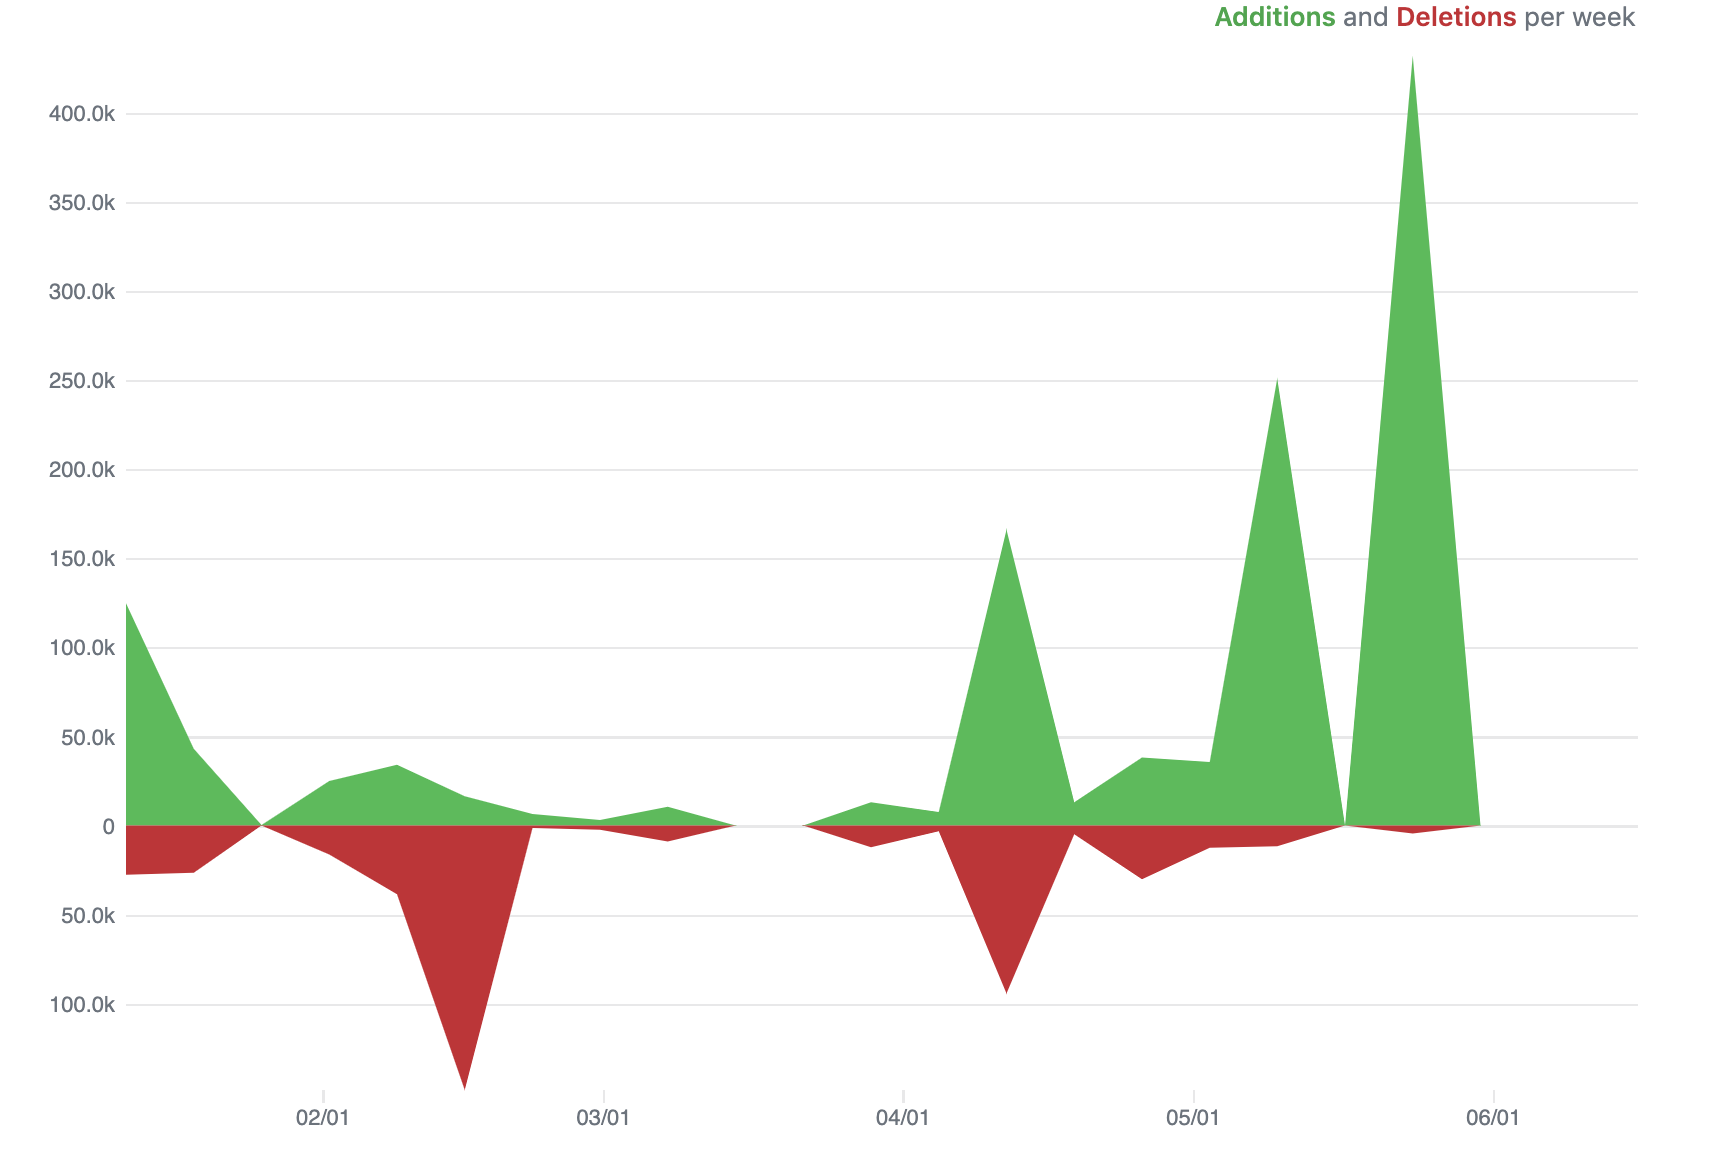
\includegraphics[width=24in]{figures/github_code_frequency}

During periods when the research team is collecting data, you would expect
a lot more additions that deletions, and you could check this plot to ensure that the
team is committing data soon after it's recorded (i.e., that there are lots of additions
on weeks with major data collection for the experiment, not several weeks after).
Periods with a lot of deletions, aren't bad, but instead likely indicate that a lot of
work is being done in editing reports and manuscripts. For example, if a paper is being
prepared for publication, you'd expect a lot of delections as the team edits it to meet
word count requirements.

The ``Insights'' page on a GitHub repository also lets you track the frequency of commits
to the project, where each commit could be something small (like fixing a typo) or
large (adding new data files for all data recorded for a timepoint for the experiment).
However, the frequency of these commits can help identify periods when the team is working
on the project. For example, the commit history graph shown below is for the GitHub
repository for a website for a spring semester course in 2020. It's clear to see the
dates when the course was in session, as well as how the project required a lot of
initial set up (shown by the number of commits early in the project period compared
to later). You can even see spring break in mid-March (the week in the middle with no
commits).

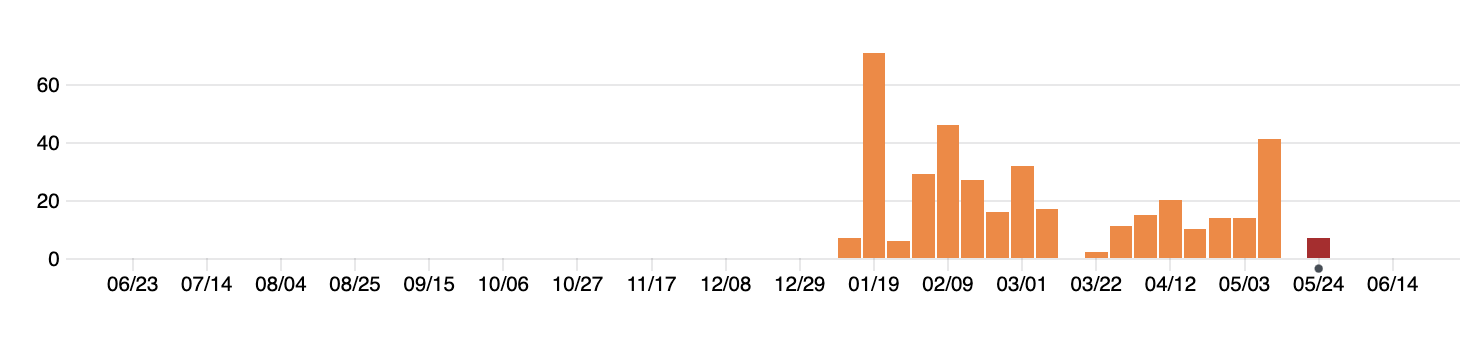
\includegraphics[width=20.53in]{figures/github_commit_frequency}

This window also allows you to track the number and timing of commits of each contributor
to the project.

\textbf{Wiki}

{[}Use the Wiki to publish information about the project, especially when you make the
project public{]}

\hypertarget{leveraging-git-and-github-as-a-scientist-who-programs}{%
\subsection{Leveraging git and GitHub as a scientist who programs}\label{leveraging-git-and-github-as-a-scientist-who-programs}}

{[}More on how to get started with GitHub if you're a programmer{]}

\begin{itemize}
\tightlist
\item
  Interfacing with RStudio
\item
  Initiating a repository and first commit
\item
  Subsequent commits and commit messages
\item
  Fixing merge conflicts when team members make concurrent changes
\item
  Using branches and forks / pull requests to try out new things
\item
  Using GitHub Actions for automation (e.g., automatic testing?)
\item
  {[}Odds and ends---.DS\_Store, \$Word\_doc{]}
\item
  More resources for learning to use git and GitHub
\end{itemize}

\hypertarget{notes}{%
\subsection{Notes}\label{notes}}

While this method of merging two sets of changes to a file generally works very well in
integrating what members of the team have typed into the file in their edits (i.e., the
actual text), it doesn't do \emph{anything} to check the logic. If that text is computer
code, then the latest version, with code integrated from two people, could be ``broken'',
even if each person confirmed that the code worked on their own computers before merging,
because a change in one spot in code could break something somewhere else in the code.
One way to try to quickly identify this kind of a problem is to create small pieces of
code that can be run whenever you'd like to check that your code is still behaving like you
want it to. These pieces of code are called ``unit tests''. They allow you to define how
you \emph{expect} your code to behave---for example, if you have created a function in your code that
counts the number of letters in a word, you expect it to always give back ``5'' for ``fever''
and ``0'' for "``. You can write a bit of code that runs the function, using inputs of''fever" and "``, and then tests to see if what it gets in return is''5" and ``0''. If it does,
great! You won't hear anything else. If it doesn't though, it will print out a message
to warn you that one of the functions in your code didn't return what you were expecting
it to.

You can collect all of these unit tests in one part of the project directory, and you
can even set up a ``hook'' with your version control program to run all of those tests
every time you merge in new changes from team members.
If everything still works fine after
merging in new changes, it will be a silent success, but if a merge breaks something,
you'll get a noisy failure which, while certainly worse that a silent success, is much,
much better than a silent failure. As Mark Twain (supposedly) said, ``What gets us into
trouble is not what we don't know. It's what we know for sure that just ain't so.''

\begin{quote}
``It is possible to put hook scripts in {[}some version control program's{]} repository
that will fire at various interesting times---notably before each commit, or after.
Hook scripts can be used for many purposes, including enforcing fine-grained access
control and sending automated commit notifications to mailing lists, bug trackers,
or even IRC channels.'' \citep{raymondunderstanding}
\end{quote}

\begin{quote}
``When the system prints the prompt \texttt{\$} and you type commands that get
executed, it's not the kernel that is talking to you, but a go-between called
the command interpreter or \emph{shell}. The shell is just an ordinary program like
\texttt{date} or \texttt{who}, although it can do some remarkable things. The fact that the shell
sits between you and the facilities of the kernel has real benefits, some of which
we'll talk about here. There are three main ones: (1) Filename shorthands: you can
pick up a whole set of filenames as arguments to a program by specifying a
pattern for the names---the shell will find the filenames that fit your pattern;
(2) Input-output redirection: you can arrange for the output of any program to
go into a file instead of onto the terminal, and for the input to come from
a file instead of the terminal. Input and output can even be connected to
other programs. (3) Personalizing the environment: you can define your own
commands and shorthands.'' \citep{kernighan1984unix}
\end{quote}

\begin{quote}
``Suppose you're typing a large document like a book. Logically this divides into many small pieces,
like chapters and perhaps sections. Physically it should be divided too, because it is cumbersome
to edit large files. Thus you should type the document as a number of files. You might have separate
files for each chapter, called `ch1', `ch2', etc. \ldots{} With a systematic naming convention, you can tell at
a glance where a particular file fits into the whole. What if you want to print the whole book? You could
say \texttt{\$\ pr\ ch1.1\ ch1.2\ ch\ 1.3\ ...}, but you would soon get bored typing filenames and start to make mistakes.
This is where filename shorthand comes in. If you say \texttt{\$\ pr\ ch*} the shell takes the \texttt{*} to mean `any
string of characters,' so ch* is a pattern that matches all filenames in the current directory that
begin with ch.~The shell creates the list, in alphabetical order, and passes the list to \texttt{pr}. The
\texttt{pr} command never sees the \texttt{*}; the pattern match that the shell does in the current directory
generates aa list of strings that are passed to \texttt{pr}. The crucial point is that filename shorthand
is not a property of the \texttt{pr} command, but a service of the shell. Thus you can use it to generate
a sequence of filenames for \emph{any} command.'' \citep{kernighan1984unix}
\end{quote}

\begin{quote}
``One of the virtues of the Unix system is that there are several ways to bring it closer to
your personal taste or the conventions of your local computing environmentl. \ldots{} If there is a file
named `.profile' in your login directory, the shell will execute the commands in it when you log in,
before printing the first prompt. So you can put commands into `.profile' to set up your environment
as you like it, and they will be executed every time you log in. \ldots{}
Some of the properties of the shell are actually controlled by so-called \emph{shell variables}, with
values that you can access and set yourself. For example, the prompt string, which we have been showing
as \texttt{\$}, is acually stored in a shell variable called `PS1', and you can set it to anything you like, like
this \texttt{PS1=\textquotesingle{}Yes\ dear?\textquotesingle{}}. \ldots{} Probably the most useful shell variable is the one that controls where the shell
looks for commands. Recall that when you type the name of a command, the shell normally looks for it
first in the current directory, then in `/bin', and then in `/usr/bin'. This sequence of directories
is called the \emph{search path}, and is stored in a shell variable called `PATH'. If the default search
path isn't what you want, you can change it, again usually in your `.profile'. \ldots{} It is also possible
to use variables for abbreviation. If you find yourself frequently referring to some directory with
a long name, it might be worthwhile adding a line like \texttt{d=/horribly/long/directory/name} to your profile,
so that you can say things like \texttt{\$cd\ \$d}. Personal variables like \texttt{d} are conventionally spelled
in lower case to distinguish them from those used by the shell itself, like \texttt{PATH}.'' \citep{kernighan1984unix}
\end{quote}

\begin{quote}
``The culmination of your login efforts is a \emph{prompt}, usually a single character, indicating that the
system is ready to accept commands from you. The prompt is most likely to be a dolloar sign or a percent
sign, but you can change it to anything you like\ldots{} The prompt is actually printed by a program called
the \emph{command interpreter} or \emph{shell}, which is your main interface to the system. \ldots{} Once you receive
the prompt, you can type \emph{commands}, which are requests that the system do something. We will use \emph{program}
as a synonym for command.'' \citep{kernighan1984unix}
\end{quote}

\begin{quote}
``While checksums are a great method to check if files are different, they don't tell
us \emph{how} the files differ. One approach to this is to compute the \emph{diff} between
two files using the Unix tool \emph{diff}. Unix's \emph{diff} works line by line, and outputs
blocks (called \emph{hunks}) that differ between files (resembling Git's \emph{git diff} command).''
\citep{buffalo2015bioinformatics}
\end{quote}

\hypertarget{applied-exercise}{%
\subsection{Applied exercise}\label{applied-exercise}}

\hypertarget{experimental-data-preprocessing}{%
\chapter{Experimental Data Preprocessing}\label{experimental-data-preprocessing}}

\hypertarget{principles-and-benefits-of-scripted-pre-processing-of-experimental-data}{%
\section{Principles and benefits of scripted pre-processing of experimental data}\label{principles-and-benefits-of-scripted-pre-processing-of-experimental-data}}

The experimental data collected for biomedical research often requires
pre-processing before it can be analyzed (e.g., gating of flow cytometry data,
feature finding / quantification for mass spectrometry data). Use of
point-and-click software can limit the transparency and reproducibility of this
analysis stage and is time-consuming for repeated tasks. We will explain how
scripted pre-processing, especially using open source software, can improve
transparency and reproducibility.

\textbf{Objectives.} After this module, the trainee will be able to:

\begin{itemize}
\tightlist
\item
  Define `pre-processing' of experimental data
\item
  Describe an open source code script and explain how it can increase
  reproducibility of data pre-processing
\end{itemize}

\hypertarget{what-is-pre-processing}{%
\subsection{What is pre-processing?}\label{what-is-pre-processing}}

Some data collected through laboratory experiments is very straightforward and
requires little or no pre-processing before it's used in analysis. For example,
{[}example{]}. Other data may require some minimal pre-processing. For example, if
you plate bacteria from a sample at a variety of dilutions, you might count each
plate and determine a measure of Colony Forming Units from the set of plates
with different dilutions by deciding which dilution provides the clearest count
and then back-calculating based on its dilution to get the total number of
colony-forming units in the original sample.

This step of pre-processing data can become much more complex with data that was
collected using complex equipment, like a flow cytometer or a mass spectrometer.
In these cases, there are often steps required to extract from the machine's
readings a biologically-relevant measurement. For example, the data output from
a mass spectrometer must be processed to move from measurements of mass and
retention time to estimates of concentrations of different molecules in the
sample. If you want to compare across multiple samples, then the preprocessing
will also involve steps to align the different samples (in terms of \ldots), as
well as to standardize the measurements for each sample, to make the
measurements from the different samples comparable. For data collected from a
flow cytometer, preprocessing may include steps to disentangle the florescence
from different markers to ensure that the read for one marker isn't inflated by
spillover florescence from a different marker.

\hypertarget{approaches-to-simple-preprocessing-tasks}{%
\subsection{Approaches to simple preprocessing tasks}\label{approaches-to-simple-preprocessing-tasks}}

There are several approaches for tackling this type of data preprocessing, to
get from the data that you initial observe (or that is measured by a piece of
laboratory equipment) to meaningful biological measurements that can be analyzed
and presented to inform explorations of a scientific hypothesis. While there are
a number of approaches that don't involve writing code scripts for this
preprocessing, there are some large advantages to scripting preprocessing any
time you are preprocessing experimental data prior to including it in figures or
further analysis. In this section, we'll describe some common non-scripted
approaches and discuss the advantages that would be brought by instead using a
code script. In the next module, we'll walk through an example of how scripts
for preprocessing can be created and applied in laboratory research.

In cases where the pre-processing is mathematically straightforward and the
dataset is relatively small, many researchers do the preprocessing by hand in a
laboratory notebook or through an equation or macro embedded in a spreadsheet.
For example, if you have plated samples at different dilutions and are trying to
calculate from these the CFUs in the original sample, this calculation is simple
enough that it could be done by hand. However, there are advantages to instead
writing a code script to do this simple preprocessing.

When you write a script to do a task with data, it is like writing a recipe that
can be applied again and again. By writing a script, you encode the process a
single time, so you can take the time to check and recheck to make sure that
you've encoded the process correctly. This helps in avoiding small errors when
you do the preprocessing---if you are punching numbers into a calculator over
and over, it's easy to mistype a number or forget a step every now and then,
while the code will ensure that the same process is run every time and that it
faithfully uses the numbers saved in the data for each step, rather than relying
on a person correctly entering each number in the calculation.

Scripts can be used across projects, as well, and so they can ensure consistency
in the calculation across projects. If different people do the calculation in
the lab for different projects or experiments, and they are doing the
calculations by hand, they might each do the calculation slightly differently,
even if it's only in small details like how they report rounded numbers. A
script will do the exact same thing every time it is applied. You can even share
your script with colleagues at other labs, if you want to ensure that your data
preprocessing is comparable for experiments conducted in different research
groups, and many scientific journals will allow supplemental material with
code used for data preprocessing and analysis, or links within the manuscript
to a repository of this code posted online.

There are also gains in efficiency when you use a script. For small
pre-processing steps, these might seem small for each experiment, and certainly
when you first write the script, it will likely take longer to write and test
the script than it would to just do the calculation by hand (even more if
you're just starting to learn how to write code scripts). However, since the
script can be applied again and again, with very little extra work to apply it
to new data, you'll save yourself time in the future, and over a lot of
experiments and projects, this can add up. This makes it particularly useful to
write scripts for preprocessing tasks that you find yourself doing again and
again in the lab.

\hypertarget{approaches-to-more-complex-preprocessing-tasks}{%
\subsection{Approaches to more complex preprocessing tasks}\label{approaches-to-more-complex-preprocessing-tasks}}

Other preprocessing tasks can be much more complex, particularly those that need
to conduct a number of steps to extract biologically meaningful measurements
from the measurements made by a complex piece of laboratory equipment, as well
as steps to make sure these measurements can be meaningfully compared across
samples.

For these more complex tasks, the equipment manufacturer will often provide
software that can be used for the preprocessing. This software might conduct
some steps using defaults, and others based on the user's specifications. These
are often provided through ``GUIs'' (graphical user interfaces), where the user
does a series of point-and-click steps to process the data. In some software,
this series of point-and-click steps is recorded as the user does them, so that
these steps can be ``re-run'' later or on a different dataset.

For many types of biological data, including output from equipment like flow
cytometers and mass spectrometers, open-source software has been developed
that can be used for this preprocessing. Often, the most cutting edge methods
for data preprocessing are first available through open-source software packages,
if the methods are developed by researchers rather than by the companies, and
often many of the algorithms that are made available through the equipment
manufacturer's proprietary software are encoded versions of an algorithm
first shared by researchers as open-source software.

It can take a while to develop a code script for preprocessing the raw data from
a piece of complex equipment like a mass spectrometer. However, the process of
developing this script requires a thoughtful consideration of the steps of
preprocessing, and so this is often time well-spent. Again, this initial time
investment will pay off later, as the script can then be efficiently applied to
future data you collect from the equipment, saving you time in pointing and
clicking through the GUI software. Further, it's easier to teach someone else
how to conduct the preprocessing that you've done, and apply it to future
experiments, because the script serves as a recipe.

When you conduct data preprocessing in a script, this also gives you access to
all the other tools in the scripting language. For example, as you work through
preprocessing steps for a dataset, if you are doing it through an R script, you
can use any of the many visualization tools that are available through R. By
contrast, in GUI software, you are restricted to the visualization and other
tools included in that particular set of software, and those software developers
may not have thought of something that you'd like to do. Open-source scripting
languages like R, Python, and Julia include a huge variety of tools, and once
you have loaded your data in any of these platforms, you can use any of these
tools.

If you have developed a script for preprocessing your raw data, it also becomes
much easier to see how changes in choices in preprocessing might influence your
final results. It can be tricky to guess whether your final results are sensitive,
for example, to what choice you make for a particular tranform for part of your
data, or in how you standardize data in one sample to make different samples
easier to compare. If the preprocessing is in a script, then you can test making
these changes and running all preprocessing and analysis scripts, to see if it
makes a difference in the final conclusions. If it does, then it helps you
identify parts of preprocessing that need to be deeply thought through for the
type of data you're collecting, and you may want to explore the documentation on
that particular step of preprocessing to determine what choice is best for your
data, rather than relying on defaults.

\hypertarget{scripting-preprocessing-tasks}{%
\subsection{Scripting preprocessing tasks}\label{scripting-preprocessing-tasks}}

Code scripts can be developed for any open-source scripting languages, including
Python, R, and Julia. These can be embedded in or called from literate programming
documents, like RMarkdown and Julia, which are described in other modules. The
word ``script'' is a good one here---it really is as if you are providing the script
for a play. In an interactive mode, you can send requests to run in the programming
language step by step using a console, while in a script you provide the whole list
of all of your ``lines'' in that conversation, and the programming language will run
them all in order without you needing to interact from the console.

For preprocessing the data, the script will have a few predictible parts. First,
you'll need to read the data in. There are different functions that can be used
to read in data from different file formats. For example, data that is stored in
an Excel spreadsheet can be loaded into R using functions in a package called
\texttt{readxl}. Data that is stored in a plain-text delimited format (like a csv file)
can be loaded into R using functions in the \texttt{readr} package.

When preprocessing data from complex equipment, you can determine how to read the
data into R by investigating the file type that is output by the equipment.
Fortunately, many types of scientific equipment follow standardized file formats.
This means that open-source developers can develop a single package that can
load data from equipment from multiple manufacturers. For example, flow cytometry
data is often stored in {[}file format{]}. Other biological datasets use file
formats that are appropriate for very large datasets and that allow R to work
with parts of the data at a time, without loading the full data in. {[}netCDF?{]}
In these cases, the first step in a script might not be to load in all the data,
but rather to provide R with a connection to the larger datafile, so it can
pull in data as it needs it.

Once the data is loaded or linked in the script, the script can proceed through
steps required to preprocess this data. These steps will often depend on the type
of data, especially the methods and equipment used to collect it. For example, for
mass spectrometry data, these steps will include \ldots{} . For flow cytometry data,
these steps would include \ldots{} .

The functions for doing these steps will often come from extensions that
different researchers have made for R. Base R is a simpler collection of data
processing and statistics tools, but the open-source framework of R has allowed
users to make and share their own extensions. In R, these are often referred to
as ``packages''. Many of these are shared through the Comprehensive R Archive
Network (CRAN), and packages on CRAN can be directly installed using the
\texttt{install.packages} function in R, along with the package's names. While CRAN
is the common spot for sharing general-purpose packages, there is a specialized
repository that is used for many genomics and other biology-related R packages
called Bioconductor. These packages can also be easily installed through a call
in R, but in this case it requires an installation function from the \texttt{BiocManager}
package. Many of the functions that are useful for preprocessing biological
data from laboratory experiments are available through Bioconductor.

Table {[}x{]} includes some of the primary R packages on Bioconductor that can be
used in preprocessing different types of biological data. There are often
multiple choices, developed by different research groups, but this list provides
a starting point of several of the standard choices that you may want to
consider as you start developing code.

Much of the initial preprocessing might use very specific functions that are
tailored to the format that the data takes once it is loaded. Later in the
script, there will often be a transfer to using more general-purpose tools in
that coding language. For example, once data is stored in a ``dataframe'' format
in R, it can be processed using a powerful set of general purpose tools
collected in a suite of packages called the ``tidyverse''. This set of packages
includes functions for filtering to specific subsets of the data, merging
separate datasets, adding new measurements for each observation that are
functions of the initial measurements, summarizing, and visualizing. The
tidyverse suite of R tools is very popular in general R use and is widely
taught, including through numerous free online resources. By moving from
specific tools to these more general tools as soon as possible in the script, a
researcher can focus his or her time in learning these general purpose tools
well, as these can be widely applied across many types of data.

By the end of the script, data will be in a format that has extracted
biologically relevant measurements. Ideally, this data will be in a general
purpose format, like a dataframe, to make it easier to work with using general
purpose tools in the scripting language when the data is used in further data
analysis or to create figures for reports, papers, and presentations. Often, you
will want to save a version of this preprocessed version of the data in your
project files, and so the last step of the script might be to write out the
cleaned data in a file that can be loaded in later scripts for analysis and
visualization. This is especially useful if these data preprocessing steps are
time consuming, as is often the case for the large raw datasets output by
laboratory equipment like flow cytometers and mass spectrometers.

Figure {[}x{]} gives an example of a data preprocessing script, highlighting these
different common areas that often show up in these scripts.

\hypertarget{potential-quotes}{%
\subsection{Potential quotes}\label{potential-quotes}}

\begin{quote}
For bioinformatics, ``all too often the software is developed without
thought toward future interoperability with other software products. As a
result, the bioinformatics software landscape is currently characterized
by fragmentation and silos, in which each research group develops and uses
only the tools created within their lab.'' \citep{barga2011bioinformatics}
\end{quote}

\begin{quote}
``The group also noted the lack of agility. Although they may be aware of
a new or better algorithm they cannot easily integrate it into their
analysis pipelines given the lack of standards across both data formats
and tools. It typically requires a complete rewrite of the code in order
to take advntge of a new technique or algorithm, requiring time and often
funding to hire developers.'' \citep{barga2011bioinformatics}
\end{quote}

\begin{quote}
``The benefit of working with a programming language is that you have the code in
a file. This means that you can easily reuse that code. If the code has
parameters it can even be applied to problems that follow a similar pattern.''
\citep{janssens2014data}
\end{quote}

\begin{quote}
``Data exploration in spreadsheet software is typically conducted via menus and
dialog boxes, which leaves no record of the steps taken.'' \citep{murrell2009introduction}
\end{quote}

\begin{quote}
``One reason Unix developers have been cool toward GUI interfaces is that, in their
designers' haste to make them `user-friendly' each one often becomes frustratingly
opaque to anyone who has to solve user problems---or, indeed, interact with it anywhere
outside the narrow range predicted by the user-interface designer.'' \citep{raymond2003art}
\end{quote}

\begin{quote}
``Many operating systems touted as more `modern' or `user friendly' than Unix achieve their
surface glossiness by locking users and developers into one interface policy, and offer an
application-programming interface that for all its elaborateness is rather narrow and rigid.
On such systems, tasks the designers have anticipated are very easy---but tasks they have
not anticipated are often impossible or at best extremely painful. Unix, on the other hand, has
flexibility in depth. The many ways Unix provides to glue together programs means that components
of its basic toolkit can be combined to produce useful effects that the designers of the individual
toolkit parts never anticipated.'' \citep{raymond2003art}
\end{quote}

\begin{quote}
``The good news is that a computer is a general-purpose machine, capable of performing
any computation. Although it only has a few kinds of instructions to work with, it can
do them blazingly fast, and it can largely control its own operation. The bad news is
that it doesn't do anything itself unless someone tells it what to do, in excruciating
detail. A computer is the ultimate sorcere's apprentice, able to follow instructions
tirelessly and without error, but requiring painstaking accuracy in the
specification of what to do.'' \citep{kernighan2011d}
\end{quote}

\begin{quote}
``\emph{Software} is the general term for sequences of instructions that make a computer
do something useful. It's `soft' in contrast with `hard' hardware, because it's
intangible, not easy to put your hands on. Hardware is quite tangible: if you drop
a computer on your foot, you'll notice. Not true for software.'' \citep{kernighan2011d}
\end{quote}

\begin{quote}
``Modern system increasingly use general purpose hardware---a processor, some memory,
and connections to the environment---and create specific behaviors by software. The
conventional wisdom is that software is cheaper, more flexible, and easier to change than
hardware is (especially once some device has left the factory).'' \citep{kernighan2011d}
\end{quote}

\begin{quote}
``An algorithm is a precise and unambiguous recipe. It's expressed in terms of a fixed
set of basic operations whose meanings are completely known and specified; it spells out
a sequence of steps using those operations, with all possible situations covered; it's
guaranteed to stop eventually. On the other hand, a \emph{program} is the opposite of
abstract---it's a concrete statement of the steps that a real computer must perform to
accomplish a task. The distinction between an algorithm and a program is like the difference
between a blueprint and a building; one is an idealization and the other is the real thing.''
\citep{kernighan2011d}
\end{quote}

\begin{quote}
``One way to view a program is as one or more algorithms expressed in a form that a computer
can process directly. A program has to worry about practical problems like inadequate memory,
limited processor speed, invalid and even malicious input data, faulty hardware, broken
network connections, and (in the background and often exacerbating the other problems)
human frailty. So if an algorithm is an idealized recipe, a program is the instructions for
a cooking robot preparing a month of meals for an army while under enemy attack.'' \citep{kernighan2011d}
\end{quote}

\begin{quote}
``During the late 1950s and early 1960s, another step was taken towards getting the
computer to do more for programmers, arguably the most important step in the history of
programming. This was the development of `high-level' programming languages that were
independent of any particular CPU architecture. High-level languages make it possible to
express computations in terms that are closer to the way a person might express them.''
\citep{kernighan2011d}
\end{quote}

\begin{quote}
``Programming in the real world tends to happen on a large scale. The strategy is similar
to what one might use to write a book or undertake any other big project: figure out what
to do, starting with a broad specification that is broken into smaller and smaller pieces,
then work on the pieces separately, while making sure that they hang together. In programming,
pieces tend to be of a size such that one person can write the precise computational steps
in some programming language. Ensuring that the pieces written by different programmers
work together is challenging, and failing to get this right is a major source of errors.
For instance, NASA's Mars Climate Orbiter failed in 1999 because the flight system software
used metric units for thrust, but course correction data was entered in English units,
causing an erroneous trajectory that brought the Orbiter too close to the planet's
surface.'' \citep{kernighan2011d}
\end{quote}

\begin{quote}
``If you're going to build a house today, you don't start by cutting down trees to make
lumber and digging clay to make your own bricks. Instead, you buy prefabricated pieces like
doors, windows, plumbing fixtures, a furnace, and a water heater. House construction is still
a big job, but it's manageable because you can build on the work of many others and rely
on an infrastructure, indeed an entire industry, that will help. The same is true of
programming. Hardly any significant program is created from nothing. Many components written
by others can be taken off the shelf and used. For instance, if you're writing a program for
Windows or a Mac, there are libraries of prefabricated menus, buttons, text editors, graphics,
network connections, database access, and so on. Much of the job is understanding the components
and gluing them together in your own way. Of course, many of these components in turn rest on
other simpler and more basic ones, often for several layers. Below that, everything runs on
the operating system, a program that manages the hardware and controls everything that happens.''
\citep{kernighan2011d}
\end{quote}

\begin{quote}
``At the simplest level, programming languages provide a mechanism called functions that make
it possible for one programmer to write code that performs a useful a useful task, then package
it in a form that other programmers can use in their programs without having to know how it
works.'' \citep{kernighan2011d}
\end{quote}

\begin{quote}
``A function has a name and a set of input data values that it needs to do its job; it does
a computation and returns a result to the part of the program that called it. \ldots{} Functions
make it possible to create a program by building on components that have been created separately
and can be used as necessary by all programmers. A collection of related functions is usually
called a \emph{library}. \ldots{} The services that a function library provides are described to programmers
in terms of an \emph{Application Programming Interface}, or \emph{API}, which lists the functions, what
they do, how to use them in a program, what input data they require, and what values they
produce. The API might also describe data structures---the organization of data that is passed
back and forth---and various other bits and pieces that all together define what a programmer
has to do to request services and what will be computed as a result. This specification must
be detailed and precise, since in the end the program will be interpreted by a dumb literal
computer, not by a friendly and accomodating human.'' \citep{kernighan2011d}
\end{quote}

\begin{quote}
``The code that a programmer writes, whether in assembly language or (much more likely) in
a high-level language, is called \emph{source code}. \ldots{} Source code is readable by other programmers,
though perhaps with some effort, so it can be studied and adapted, and any innovations or ideas
it contains are visible.'' \citep{kernighan2011d}
\end{quote}

\begin{quote}
``In early times, most software was developed by companies and most source code was
unavailable, a trade secret of whoever developed it.'' \citep{kernighan2011d}
\end{quote}

\begin{quote}
``An \emph{operating system} is the software underpinning that manages the hardware of a
computer and makes it possible to run other programs, which are called \emph{applications}.
\ldots{} It's a clumsy but standard terminology for programs that are more or less self-contained
and focused on a single task.'' \citep{kernighan2011d}
\end{quote}

\begin{quote}
``Software, like many other things in computing, is organized into layers, analogous to
geological strata, that separate one concern from another. Layering is one of the important
ideas that help programmers to manage complexity.'' \citep{kernighan2011d}
\end{quote}

\begin{quote}
``I think that it's important for a well-informed person to know something about
programming, perhaps only that it can be surprisingly difficult to get very simple
programs working properly. There is nothing like doing battle with a computer to teach
this lesson, but also to give people a taste of the wonderful feeling of accomplishment
when a program does work for the first time. It may also be valuable to have enough
programming experience that you are cautious when someone says that programming is easy,
or that there are no errors in a program. If you have trouble making 10 lines of code
work after a day of struggle, you might be legitimately skeptical of someone who claims
that a million-line program will be delivered on time and bug-free.'' \citep{kernighan2011d}
\end{quote}

\begin{quote}
``Programming languages share certain basic ideas, since they are all notations for spelling
out a computation as a sequence of steps. Every programming language thus will provide ways
to get input data upon which to compute; do arithmetic; store and retrieve intermediate
values as computation proceeds; display results along the way; decide how to proceed on the basis
of previous computations; and save results when the computation is finished. Languages have
\emph{syntax}, that is, rules that define what is grammatically legal and what is not.
Programming languages are picky on the grammatical side: you have to say it right or there
will be a complaint. Languages also have \emph{semantics}, that is, a defined meaning for every
construction in the language.'' \citep{kernighan2011d}
\end{quote}

\begin{quote}
``In programming, a \emph{library} is a collection of related pieces of code. A library typically
includes the code in compiled form, along with needed source code declarations {[}for C++{]}.
Libraries can include stand-alone functions, classes, type declarations, or anything else that
can appear in code.'' \citep{spraul2012think}
\end{quote}

\begin{quote}
``One way to write R code is simply to enter it interactively at the command line\ldots{} This
interactivity is beneficial for experimenting with R or for exploring a data set in a casual
manner. \ldots{} However, interactively typing code at the R command line is a very bad approach from
the perspective of recording and documenting code because the code is lost when R is shut down.
A superior approach in general is to write R code in a file and get R to read the code from the file.'' \citep{murrell2009introduction}
\end{quote}

\begin{quote}
``The features of R are organized into separate bundles called \emph{packages}. The standard R
installation includes about 25 of those packages, but many more can be downloaded from CRAN and
installed to expand the things that R can do. \ldots{} Once a package is installed, it must be
\emph{loaded} within an R session to make the extra features available. \ldots{} Of the 25 packages
that are installed by default, nine packages are \emph{loaded} by default when we start a new
R session; these provide the basic functionality of R. All other packages must be loaded
before the relevant features can be used.'' \citep{murrell2009introduction}
\end{quote}

\begin{quote}
``The R environment is the software used to run R code.'' \citep{murrell2009introduction}
\end{quote}

\hypertarget{discussion-questions}{%
\subsection{Discussion questions}\label{discussion-questions}}

\hypertarget{introduction-to-scripted-data-pre-processing-in-r}{%
\section{Introduction to scripted data pre-processing in R}\label{introduction-to-scripted-data-pre-processing-in-r}}

We will show how to implement scripted pre-processing of experimental data
through R scripts. We will demonstrate the difference between interactive coding
and code scripts, using R for examples. We will then demonstrate how to create,
save, and run an R code script for a simple data cleaning task.

\textbf{Objectives.} After this module, the trainee will be able to:

\begin{itemize}
\tightlist
\item
  Describe what an R code script is and how it differs from interactive
  coding in R
\item
  Create and save an R script to perform a simple data pre-processing task
\item
  Run an R script
\item
  List some popular packages in R for pre-processing biomedical data
\end{itemize}

\hypertarget{subsection-1}{%
\subsection{Subsection 1}\label{subsection-1}}

\hypertarget{subsection-2}{%
\subsection{Subsection 2}\label{subsection-2}}

\hypertarget{applied-exercise}{%
\subsection{Applied exercise}\label{applied-exercise}}

\hypertarget{simplify-scripted-pre-processing-through-rs-tidyverse-tools}{%
\section{Simplify scripted pre-processing through R's `tidyverse' tools}\label{simplify-scripted-pre-processing-through-rs-tidyverse-tools}}

The R programming language now includes a collection of `tidyverse' extension
packages that enable user-friendly yet powerful work with experimental data,
including pre-processing and exploratory visualizations. The principle behind
the `tidyverse' is that a collection of simple, general tools can be joined
together to solve complex problems, as long as a consistent format is used for
the input and output of each tool (the `tidy' data format taught in other
modules). In this module, we will explain why this `tidyverse' system is so
powerful and how it can be leveraged within biomedical research, especially for
reproducibly pre-processing experimental data.

\textbf{Objectives.} After this module, the trainee will be able to:

\begin{itemize}
\tightlist
\item
  Define R's `tidyverse' system
\item
  Explain how the `tidyverse' collection of packages can be both user-friendly
  and powerful in solving many complex tasks with data
\item
  Describe the difference between base R and R's `tidyverse'.
\end{itemize}

\hypertarget{limitations-of-object-oriented-programming}{%
\subsection{Limitations of object-oriented programming}\label{limitations-of-object-oriented-programming}}

In previous sections, we described how the R programming language allows for
object-oriented programming, and how customized objects are often used in
preprocessing for biological data. This is a helpful approach for preprocessing,
because it can handle complexities in biological data at its early stages of
preprocessing, when R must handle complex input formats from equipment like
flow cytometers or mass spectrometers, and data sizes that are often very large.

However, once you have preprocessed your data, it is often possible to work with it
in a smaller, more consistent object type. This will give you a lot of flexibility
and power. While object-oriented approaches can handle complex data, it can be a
little hard to write and work with code that is built on an object oriented approach.
Working with this type of code requires you to keep track of what object type your
data is in at each stage of a code pipeline, as well as which functions can work with
that type of object.

Further, this type of coding, in practice at least, can be a bit inflexible.
Often, specific functions only work with a single or few types of functions. In
theory, object-oriented programming allows for \emph{methods} that work in customized
ways with different types of objects to apply customized code to that type of
object for similar, common-sense results. For example, there are often \texttt{summary}
and \texttt{plot} methods for most types of objects, and these apply code that is
customized to that object type and output, respectively, summarized information
about the data in the object and a plot of the data in the object. However, when
you want to do more with the object that summarize it or create its default
plot, you often end up needing to move to more customized functions that work
only with a single or few object types. When you get to this point, you find that
you have to remember which functions work with which object type, and you have to
use different functions at different stages of your code pipeline, as your code
changes from one object class to another.

Further, many of these functions input one object type and output a different
one. This evolution of object types for storing data can be difficult to navigate
and keep track of. Different object types store data in different ways, and so
this evolution of data object types for storage can make it tricky to figure out
how to extract and explore data along the pipeline. It makes it hard to write your
own code to explore and visualize the data along the way, as well, and so users
are often restricted to the visualization and analysis functions pre-made and
shared in packages when working with data in complex object types, especially
until the user becomes very comfortable with coding in R.

Overall, what does this all mean? Object-oriented approaches offer real advantages
early in the process of pre-processing biological data, especially complex and
large data output from complex laboratory equipment. However, once this pre-processing
is completed, there is a big advantage in moving the data into a simple format
and then continuing coding, data analysis, and visualization using tools that
work with this simple format. This is the approach taken by a suite of R packages
called the ``tidyverse'', as well as extensions that build off the approach that
this suite of tools embraces. This ``tidyverse'' approach is described in the
next section.

\hypertarget{the-tidyverse-approach}{%
\subsection{The ``tidyverse'' approach}\label{the-tidyverse-approach}}

The term ``elegance'' often captures styles and approaches that are beautiful and
functional without unneeded extras or complexity. Engineers and scientists
sometimes use this term to capture approaches that achieve a desired result with
minimal complexity and friction. A coding problem, for example, could be solved
by an average coder with a hundred lines of code that get the job done, but a
very good coder might be able to solve the same problem with five lines of code
that are easy to follow. The second approach would be applauded as the ``elegant''
solution. In mathematics, similarly, proofs can be complex and unwieldy, or they
can be simple and elegant---this idea was beautifully captured by the Hungarian
mathematician Paul Erdos, who famously described very elegant mathematical proofs
as being from ``The Book''---that is, God's own version of the proof of the
mathematical idea.

\begin{quote}
``Paul Erdos liked to talk about The Book, in which God maintains the perfect
proofs for mathematical theorems, following the dictum of G. H. Hardy that
there is no permanent place for ugly mathematics. Erdos also said that you
need not believe in God but, as a mathematician, you should believe in
The Book.'' {[}Proofs from the Book, Third Edition, Preface{]}
\end{quote}

The ``tidyverse'' approach in R is elegant. It is powerful, and gives you immense
flexibility once you've gotten the hang of it, but it's also so straightforward
that the basics can be quickly taught to and applied by beginning coders. It
focuses on keeping data in a simple, standard format called ``tidy'' dataframes.
By keeping data in this format while working with it, common tools can be applied
that work with the data at any stage of a ``tidy'' coding pipeline. These tools take
a ``tidy'' dataframe as their input, and they also output a ``tidy'' dataframe, with
whatever change the function implements applied. Because each of these ``tidyverse''
tools input and output data in the same standard format, they can be strung together
in order you want. By contrast, when functions input and output data in different
object types, they can only be joined in a specified order, because you can only
apply certain functions to certain object types.

Since the ``tidyverse'' tools can be strung together in any order, they can be
used very flexibly to build up to do interesting tasks. The tidyverse tools
generally each do very small and simple things. For example, one function
(\texttt{select}) just limits the data to a subset of its original columns; another
(\texttt{mutate}) adds or changes values in columns of the dataset, while another
(\texttt{distinct}) limits the dataframe to remove any rows that are duplicates. These
small, simple steps can be combined together in different patterns to add up to
complex operations on the data, while keeping each step very simple and clear.
Since the data stays in a standard and simple object type, it is easy to check
in on your data at any stage, as the common visualization tools for this
approach (from the \texttt{ggplot2} package and its extensions) can be always be
applied to data stored in a tidy dataframe.

The centralizing principal of the tidyverse approach is the format in which data
is stored throughout ``tidyverse'' coding---the tidy dataframe. We've described
this data type, including its rules and advantages, in an earlier module of this
book. Briefly, you can think of this format in two parts. First, there's the R
object type that the data should be stored in---a basic ``dataframe'' object. The
dataframe object type is a very basic two-dimensional format for storing data in
R. When you print it out, it will remind you of looking at data in a
spreadsheet. The two dimensions---rows and columns---allow you to include data
for one or more observations, with different values that were measured for each.
For example, if you were conducting a study of children's BMI and blood sugar,
you might have an observation for each child in the study, and values measured
for each child of height, weight, a blood sugar measure, study ID, and date of
the observation.

The two-dimensional structure of a dataframe keeps the values
measured for each observation lined up with each other, and lets you keep them
aligned as you work with the data. You could also store data for each value as
separate objects, in one-dimensional vectors, which you can visualize as strings
of values of the same data type, like the dates that each observation was made,
or the weight of each study subject. However, when the data is in separate
vectors, it is easy to make coding mistakes, and coding is often less efficient.
If you want to remove one observation, for example, because you find it is a
duplicate, you would need to carefully make sure you remove it correctly from
each vector. When data are stored in a dataframe, you can remove the row for
that observation with one command, and you can be sure that you've removed the
value you meant to from each of the measured values.

Sometimes, you'll see that data in a tidyverse approach are stored in a special
type of dataframe called a ``tibble''---this isn't very different from a
dataframe, and in fact is a special type of dataframe. It's only differences in
practice are that it has a slightly different \texttt{print} method. The \texttt{print} method
is the method that's run, by default, when you just type the R object's name
at the console. A tibble prints more nicely than a basic dataframe. By default,
it will only print the first few lines. By contrast, a dataframe will, by default,
print everything---if you have a lot of data, this can create an overwhelming
amount of output when you just want to check out what the data looks like. The
printout of a tibble will also include some interesting annotations to help you
see what's in the data, including the dimensions of the full dataframe and the
data type of each column in the data.

The R object class---dataframe, and more specifically, tibble---of the standard
format for data for a tidyverse approach is just the first part of the standard
data format for the tidyverse approach. The second part of the standard format is
how you organize your data in this format. To easily work with tidyverse functions,
you'll want to make sure that your data is stored within that dataframe following
``tidy'' data principals. These are fully described in an earlier module in this
book {[}which module{]}. If you use this data format to initially collect your
data, as described in an earlier module, you will find it very easy to read the
data into R and work within the tidyverse approach. When working with larger and
more complex data collected from laboratory equipment, you may find you need to
do some preprocessing of the data using an object-oriented approach before you
can move the data into this tidy format, but at that point, you can continue with
analysis and visualization of your data using a tidyverse approach.

\hypertarget{how-to-tidyverse}{%
\subsection{How to ``tidyverse''}\label{how-to-tidyverse}}

Once data are in the ``tidy'' data format, you can create a pipeline of code that
uses small tools, each of which does one simple thing, to work with the data.
This work can include cleaning the data, adding values that are functions of the
original values for each observation (e.g., adding a column with BMI based on
values for each observation on height and weight), applying statistical models to
test hypotheses, summarizing data to create tables, and visualizing the data.

The tidyverse approach is now widely taught, both in in-person courses at
universities and through a variety of online resources. One key resource for
learning the tidyverse approach for R is the book \emph{R for Data Science} by Hadley
Wickham (the primary developer of the tidyverse) and Garrett Grolemund. This
book is available as a print edition through O'Reilly Media. It is also freely
available online at \url{https://r4ds.had.co.nz/}. This book is geared to beginners in
R, moving through to get readers to an intermediate stage of coding expertise,
which is a level that will allow most scientific researchers to powerfully
work with their experimental data. The book includes exercises for practicing the
concepts, and a separate online book is available with solutions for the
exercises (\url{https://jrnold.github.io/r4ds-exercise-solutions/}).

{[}More on other resources for learning the tidyverse.{]}

Since there are so many excellent resources available---many for free---to learn
how to code in R using the tidyverse approach, we consider it beyond the scope
of these modules to go more deeply into these instructions. However, we do think
it is critical that biological researchers learn how to connect this approach to
the type of coding that is often necessary for pre-processing large and complex
data that is output from laboratory equipment. Through many of the modules in this book,
we provide advice on how to make these connections, so that data from different
sources---including different types of laboratory equipment and hand-recorded data
collected by personnel in the lab, like colony forming units measured from plating
samples---can all be connected in a tidyverse pipeline by recording hand-recorded
data following a tidy format and by pre-processing data with the aim of moving
data toward a tidy dataframe that can be integrated with other ``tidy'' data for
analysis and visualization.

\hypertarget{subsection-1}{%
\subsection{Subsection 1}\label{subsection-1}}

\begin{quote}
``There is a now-old trope in the world of programming. It's called the `worse is
better' debate; it seeks to explain why the Unix operating systems (which include
Mac OS X these days), made up of so many little interchangeable parts, were so much
more successful in the marketplace than LISP systems, which were ideologically pure,
based on a single languagae (again, LISP), which itself was exceptionally simple,
a favorite of `serious' hackers everywhere. It's too complex to rehash here, but one
of the ideas inherent within `worse is better' is thata systems made up of many
simple pieces that can be roped together, even if those pieces don't share a consistent
interface, are likely to be more successful than systems that are designed with consistency
in every regard. And it strikes me that this is a fundamental drama of new technologies.
Unix beat out the LISP machines. If you consider mobile handsets, many of which run
descendants of Unit (iOS and Andriod), Unix beat out Windows as well. And HTML5 beat out
all of the various initiatives to create a single unified web. It nods to accessibility:
it doesn't get in the way of those who want to make something huge and interconnected.
But it doesn't enforce; it doesn't seek to change the behavior of page creators in the
same way that such lost standards as XHTML 2.0 (which eremged from the offices of
the World Wide Web Consortium, and then disappeared under the weight of its own
intentions) once did. It's not a bad place to end up. It means that there is no
single framework, no set of easy rules to lear, no overarching principles that,
once learned, can make the web appear like a golden statue atop a mountain. There
are just components: HTML to get the words on the page, forms to get people to
write in, videos and images to put up pictures, moving or otherwise, and
JavaScript to make everything dance.'' \citep{ford2015on}
\end{quote}

\begin{quote}
``One of the fundamental contributions of the Unix system {[}is{]} the idea of a \emph{pipe}.
A pipe is a way to connect the output of one program to the input of another program
without any temporary file; a \emph{pipeline} is a connection of two or more programs through
pipes. \ldots{} Any program that reads from a terminal can read from a pipe instead; any program
that writes on the terminal can write to a pipe. \ldots{} The programs in a pipeline actually
run at the same time, not one after another. This means that the programs in a pipeline
can be interactive; the kernel looks after whatever scheduling and synchronization is needed
to make it all work. As you probably suspect by now, the shell arranges things when you
ask for a pipe; the individual programs are oblivious to the redirection.'' \citep{kernighan1984unix}
\end{quote}

\begin{quote}
``Even though the Unix system introduces a number of innovative programs and techniques,
no single program or idea makes it work well. Instead, what makes it effective is an approach
to programming, a philosophy of using the computer. Although that philosophy can't be written
down in a single sentence, at its heart is the idea that the power of a system comes more from
the relationships among programs than from the programs themselves. Many Unix programs do
quite trivial things in isolation, but, combined with other programs, become general and
useful tools.'' \citep{kernighan1984unix}
\end{quote}

\begin{quote}
``What is `Unix'? In the narrowest sense, it is a time-sharing operating system \emph{kernel}:
a program that controls the resources of a computer and allocates them among its users.
It lets users run their programs; it controls the peripheral devices (discs, terminals,
printers, and the like) connected to the machine; and it provides a file system that
manages the long-term storage of information such as programs, data, and documents.
In a broader sense, `Unix' is often taken to include not only the kernel, but also
essential programs like compiles, editors, command languages, programs for copying and
printing files, and so on. Still more broadly, `Unix' may even include programs
develpoed by you or others to be run on your system, such as tools for document
preparation, routines for statistical analysis, and graphics packages.'' \citep{kernighan1984unix}
\end{quote}

\hypertarget{subsection-2}{%
\subsection{Subsection 2}\label{subsection-2}}

\hypertarget{practice-quiz}{%
\subsection{Practice quiz}\label{practice-quiz}}

\hypertarget{complex-data-types-in-experimental-data-pre-processing}{%
\section{Complex data types in experimental data pre-processing}\label{complex-data-types-in-experimental-data-pre-processing}}

Raw data from many biomedical experiments, especially those that use
high-throughput techniques, can be very large and complex. Because of the scale
and complexity of these data, software for pre-processing the data in R often
uses complex, `untidy' data formats. While these formats are necessary for
computational efficiency, they add a critical barrier for researchers wishing to
implement reproducibility tools. In this module, we will explain why use of
complex data formats is often necessary within open source pre-processing
software and outline the hurdles created in reproducibility tool use among
laboratory-based scientists.

\textbf{Objectives.} After this module, the trainee will be able to:

\begin{itemize}
\tightlist
\item
  Explain why R software for pre-processing biomedical data often stores
  data in complex, `untidy' formats
\item
  Describe how these complex data formats can create barriers to
  laboratory-based researchers seeking to use reproducibility tools for
  data pre-processing
\end{itemize}

\hypertarget{subsection-1}{%
\subsection{Subsection 1}\label{subsection-1}}

When you process data using a programming language, there will be different
structures that you can use to store data as you work with it. In other modules,
we've discussed the ``tidyverse'' approach to processing data in R---this approach
emphasizes the dataframe as a way to store data while you're working with it.
In fact, its use of this data structure for data storage is one of the defining
features of the ``tidyverse'' approach.

Data in R can be stored in a variety of other formats, too. When you are working
with biological data---in particular, complex or large data output from laboratory
equipment---there can be advantages to using data structures besides dataframes.
In this section, we'll discuss some of the complex characteristics of biomedical
data that recommend the use of data structures in R beyond the dataframe. We'll
also discuss how the use of these other data structures can complicate the use of
``tidyverse'' functions and principles that you might learn in beginning R programming
courses and books. In later modules, we'll discuss how to connect your work in R
to clean and analyze data by performing earlier pre-processing steps using more
complex data structures and then transferring when possible to dataframes for
storing data, to allow you to take advantage of the power and ease of the
``tidyverse'' approach as early as possible in your pipeline.

\hypertarget{subsection-2}{%
\subsection{Subsection 2}\label{subsection-2}}

There are two main features of biomedical data---in particular, data collected from
laboratory equipment like flow cytometers and mass spectrometers---that make it
useful to use more complex data structures in R in the earlier stages of preprocessing
the data. First, the data are often very large, in some cases so large that it is
difficult {[}or impossible?{]} to read them into R. Second, the data might combine
various elements, each with their own natural structures, that you'd like to keep
together as you move through the steps of preprocessing the data.

{[}Data size{]}

{[}Different elements in the data{]}
Most laboratory equipment can output a raw data file that you can then read into R.
For many types of laboratory equipment, these raw data files follow a strict format.
For example {[}flow cytometery format\ldots{]}\ldots{}

The file formats will often have different pieces of data stored in specific spots.
For example, the equipment might record not only the measurements taken for the
sample, but also information about the setting that were applied to the equipment
while the measurements were taken, the date of the measurements, and other metadata
that may be useful to access when preprocessing the data. Each piece of data may
have different ``dimensions''. For example, the measurements might provide one
measurement per metabolite feature or per marker. Some metadata might also be
provided with these dimensions (e.g., metadata about the markers for flow
cytometry data), but other metadata might be provided a single time per sample
or even per experiment---for example, the settings on the equipment when the
sample or samples were run.

When it comes to data structures, dataframes and other two-dimensional data storage
structures (you can visualize these as similar to the format of data in a spreadsheet,
with rows and columns) work well to store data where all data conform to a common
dimension. For example, a dataframe would work well to store the measurements
for each marker in each sample in a flow cytometry experiment. In this case,
each column could store the values for a specific marker and each row could
provide measurements for a sample. In this way, you could read the measurements
for one marker across all samples by reading down a column, or read the measurements
across all markers for one sample by reading across a row.

When you have data that doesn't conform to these common dimensions {[}unit of
measurement?{]} however, a dataframe may work poorly to store the data. For
example, if you have measurements taken at the level of the equipment settings
for the whole experiment, these don't naturally fit into the dataframe format.
In the ``tidyverse'' approach, one approach to handling data with different units
of measurement is to store data for each unit of measurement in a different
dataframe and to include identifiers that can be used to link data across the
dataframes. More common, however, in R extensions for preprocessing biomedical
data is to use more complex data structures that can store data with different
units of measurement in different slots within the data structure, and use these
in conjunction with specific functions that are built to work with that specific
data structure, and so know where to find each element within the data
structure.

\hypertarget{subsection-3}{%
\subsection{Subsection 3}\label{subsection-3}}

\hypertarget{practice-quiz}{%
\subsection{Practice quiz}\label{practice-quiz}}

\hypertarget{complex-data-types-in-r-and-bioconductor}{%
\section{Complex data types in R and Bioconductor}\label{complex-data-types-in-r-and-bioconductor}}

Many R extension packages for pre-processing experimental data use complex
(rather than `tidy') data formats within their code, and many output data in
complex formats. Very recently, the \emph{broom} and \emph{biobroom} R
packages have been developed to extract a `tidy' dataset from a complex data
format. These tools create a clean, simple connection between the complex data
formats often used in pre-processing experimental data and the `tidy' format
required to use the `tidyverse' tools now taught in many introductory R courses.
In this module, we will describe the `list' data structure, the common backbone
for complex data structures in R and provide tips on how to explore and extract
data stored in R in this format, including through the \emph{broom} and
\emph{biobroom} packages.

\textbf{Objectives.} After this module, the trainee will be able to:

\begin{itemize}
\tightlist
\item
  Describe the structure of R's `list' data format
\item
  Take basic steps to explore and extract data stored in R's complex, list-based
  structures
\item
  Describe what the \emph{broom} and \emph{biobroom} R packages can do
\item
  Explain how converting data to a `tidy' format can improve reproducibility
\end{itemize}

\hypertarget{subsection-1}{%
\subsection{Subsection 1}\label{subsection-1}}

\begin{quote}
``Object-oriented design doesn't have to be over-complicated design, but we've
observed that too often it is. Too many OO designs are spaghetti-like tangles of
is-a and has-a relationships, or feature thick layers of glue in which many of the
objects seem to exist simply to hold places in a steep-sided pyramid of abstractions.
Such designs are the opposite of transparent; they are (notoriously) opaque and
difficult to debug.'' \citep{raymond2003art}
\end{quote}

\begin{quote}
``Unix programmers are the original zealots about modularity, but tend to go about it
in a quiter way {[}that with OOP{]}. Keeping glue layers thin is part of it; more generally,
our tradition teaches us to build lower, hugging the ground with algorithms and structures
that are designed to be simple and transparent.'' \citep{raymond2003art}
\end{quote}

\begin{quote}
``A \emph{standard} is a precise and detailed description of how some artifact is built
or is supposed to work. Examples of software standards include programming
languages (the definition of syntax and semantics), data formats (how information is
represented), algorithmic processing (the steps necessary to do a computation), and
the like. Some standards, like the Word \texttt{.doc} file format, are \emph{de facto} standards---they
have no official standing but everyoen uses them. The word `standard' is best reserved for
formal descriptions, often developed and maintained by a quasi-neutral party like a
government or a consortium, that define how something is built or operated. The definition
is sufficiently complete and precise that separate entities can interact or provide independent
implementations. We benefit from hardware standards all the time, though we may not notice
how many there are. If I buy a new television set, I can plug it inot the electrical outlets
in my home thanks to standards for the size and shape of plugs and the voltage they provide.
The set itself will receive signals and display pictures because of standards for broadcast
and cable television. I can plug other devices into it through standard cables and connectors
like HDMI, USB, S-video and so on. But every TV needs its own remote control and every cell
phone needs a different charger because those have not been standardized. Computing has plenty
of standards as well, including character sets like ASCII and Unicode, programming languages
like C and C++, algorithms for encryption and compression, and protocols for exchanging
information over networks.'' \citep{kernighan2011d}
\end{quote}

\begin{quote}
``Standards are important. They make it possible for independently created things to cooperate,
and they open an area to competition from multiple suppliers, while proprietary systems tend
to lock everyone in. \ldots{} Standards have disadvantages, too---a standard can impede progress if
it is inferior or outdated yet everyone is forced to use it. But these are modest drawbacks
compared to the advantages.'' \citep{kernighan2011d}
\end{quote}

\begin{quote}
``A \emph{class} is a blueprint for constructing a particular package of code and data; each
variable created according to a class's blueprint is known as an \emph{object} of that class.
Code outside of a class that creates and uses an object of that class is known as a \emph{client}
of the class. A \emph{class declaration} names the class and lists all of the \emph{members}, or
items inside that class. Each item is either a \emph{data member}---a variable declared within the
class---or a \emph{method} (also known as a \emph{member function}), which is a function declared within
the class. Member functions can include a special type called a \emph{constructor}, which has the
same name as the class and is invoked implicitly when an object of the class is declared.
In addition to the normal attributes of a variable or function declaration (such as type, and
for functions, the parameter list), each member has an \emph{access specifier}, which indicates
what functions can access the member. A \emph{public member} can be accessed by any code using the
object: code inside the class, a client of the class, or code in a \emph{subclass}, which is a class
that `inherits' all the code and data of an existing class. A \emph{private member} can be
accessed only by the code inside the class. \emph{Protected members} \ldots{} are similar to private
members, except that methods in subclasses can also reference them. Both private and
protected members, though, are inaccessible from client code.'' \citep{spraul2012think}
\end{quote}

\begin{quote}
``An object should be a meaningful, closely knit collection of data and code that operates
on the data.'' \citep{spraul2012think}
\end{quote}

\begin{quote}
``Recognizing a situation in which a class would be useful is essential to reaching the
higher levels of programming style, but it's equally important to recognize situations in
which a class is going to make things worse.'' \citep{spraul2012think}
\end{quote}

\begin{quote}
``The word \emph{encapsulation} is a fancy way of saying that classes put multiple pieces of
data and code together in a single package. If you've ever seen a gelatin medicine capsule
filled with little spheres, that's a good analogy: The patient takes one capsule and swallows
all the individual ingredient spheres inside. \ldots{} From a problem-solving standpoint,
encapsulation allows us to more easily reuse the code from previous problems to solve current
problems. Often, even though we have worked on a problem similar to our current project,
reusing what we learned before still takes a lot of work. A fully encapsulated class can
work like an external USB drive; you just plug it in and it works. FOr this to happen,
though, we must design the class correctly to make sure that the code and data is truly
encapsulated and as independent as possible from anything outside of the class. For example,
a class that references a global variable can't be copied into a new project without
copying the global variable, as well.'' \citep{spraul2012think}
\end{quote}

\begin{quote}
``Beyond reusing classes from one program to the next, classes offer the potential for
a more immediate form of code reuse: inheritance. \ldots{} Using inheritance, we create parent
classes with methods common to two or more child classes, thereby `factoring out' not
just a few lines of code {[}as with helper functions in procedural code{]} but whole methods.''
\citep{spraul2012think}
\end{quote}

\begin{quote}
``One technique we're returned to again and again is dividing a complex problem into
smaller, more manageable pieces. Classes are great at dividing programs up into functional
units. Encapsulation not only holds data and code together in a reusable package; it also
cordons off that data and code from the rest of the program, allowing us to work on that
class, and everything else separately. The more classes we make in a program, the greater
the problem-dividing effect.'' \citep{spraul2012think}
\end{quote}

\begin{quote}
``Some people use the terms \emph{information hiding} and \emph{encapsulation} interchangeable, but
we'll separate the ideas here. As described previously \ldots, encapsulation is
packaging data and code together. Information hiding means separating the interface of a
data structure---the definition of the operations and their parameters---from the implementation
of a data structure, or the code inside the functions. If a class has been written with
information hiding as a goal, then it's possible to change the implementation of the methods
without requiring any changes in the client code (the code that uses the class). Again, we
have to be clear on the term \emph{interface}; this means not only the name of the methods and
their parameter list but also the explanation (perhaps expressed in code documentation) of
what the different methods do. When we talk about changing the implementation without
changing the interface, we mean that we change \emph{how} the class methods work but not
\emph{what} they do. Some programming authors have referred to this as a kind of implicit contract
between the class and the client: The class agrees never to change the effects of
existing operations, and the client agrees to use the class strictly on the basis of its
interface and to ignore any implementation details.'' \citep{spraul2012think}
\end{quote}

\begin{quote}
``So how does information hiding affect problem solving? The principle of information hiding
tells the programmer to put aside the class implementation details when working on the
client code, or more broadly, to be concerned about a particular class's implementation
only when working inside that class. When you can put implementation details out of your
mind, you can eliminate distracting thoughts and concentrate on solving the problem at hand.''
\citep{spraul2012think}
\end{quote}

\begin{quote}
``A final goal of a well-designed class is expressiveness, or what might be broadly called
writability---the ease with which code can be written. A good class, once written, makes
the rest of the code simpler to write in the way that a good function makes code simpler to
write. Classes effectively extend a language, becoming high-level counterparts to basic
low-level features such as loops, if statements, and so forth. \ldots{} With classes, programming
actions that previously took many steps can be done in just a few steps or just one.''
\citep{spraul2012think}
\end{quote}

\begin{quote}
"When we are writing code in a programming language, we work most of the time with RAM,
combining and restructuring data values to produce new values in RAM. \ldots{} The computer memory
in RAM is a series of 0's and 1's, just like the computer memory used to store files in mass
storage. In order to work with data values, we need to get those values into RAM in some
format. At the basic level of representing a single number or a single piece of text, the
solution is the same as it was in Chapter 5 {[}on file formats for mass storage{]}. Everything
is represented as a pattern of bits, using various numbers of bytes for different sorts of
values. In R, in an English locale, and on a 32-bit operating system, a single character
usually takes up one byte, an
\end{quote}

\hypertarget{subsection-2}{%
\subsection{Subsection 2}\label{subsection-2}}

\hypertarget{applied-exercise}{%
\subsection{Applied exercise}\label{applied-exercise}}

\hypertarget{example-converting-from-complex-to-tidy-data-formats}{%
\section{Example: Converting from complex to `tidy' data formats}\label{example-converting-from-complex-to-tidy-data-formats}}

We will provide a detailed example of a case where data pre-processing in R
results in a complex, `untidy' data format. We will walk through an example of
applying automated gating to flow cytometry data. We will demonstrate the
complex initial format of this pre-processed data and then show trainees how a
`tidy' dataset can be extracted and used for further data analysis and
visualization using the popular R `tidyverse' tools. This example will use real
experimental data from one of our Co-Is research on the immunology of
tuberculosis.

\textbf{Objectives.} After this module, the trainee will be able to:

\begin{itemize}
\tightlist
\item
  Describe how tools like \textit{biobroom} were used in this real research
  example to convert from the complex data format from pre-processing to a format
  better for further data analysis and visualization
\item
  Understand how these tools would fit in their own research pipelines
\end{itemize}

\hypertarget{subsection-1}{%
\subsection{Subsection 1}\label{subsection-1}}

\hypertarget{subsection-2}{%
\subsection{Subsection 2}\label{subsection-2}}

\hypertarget{applied-exercise}{%
\subsection{Applied exercise}\label{applied-exercise}}

\hypertarget{introduction-to-reproducible-data-pre-processing-protocols}{%
\section{Introduction to reproducible data pre-processing protocols}\label{introduction-to-reproducible-data-pre-processing-protocols}}

Reproducibility tools can be used to create reproducible data pre-processing
protocols---documents that combine code and text in a `knitted' document, which
can be re-used to ensure data pre-processing is consistent and reproducible
across research projects. In this module, we will describe how reproducible data
pre-processing protocols can improve reproducibility of pre-processing
experimental data, as well as to ensure transparency, consistency, and
reproducibility across the research projects conducted by a research team.

\textbf{Objectives.} After this module, the trainee will be able to:

\begin{itemize}
\tightlist
\item
  Define a `reproducible data pre-processing protocol'
\item
  Explain how such protocols improve reproducibility at the data pre-processing
  phase
\item
  List other benefits, including improving efficiency and consistency of data
  pre-processing
\end{itemize}

\hypertarget{subsection-1}{%
\subsection{Subsection 1}\label{subsection-1}}

\hypertarget{subsection-2}{%
\subsection{Subsection 2}\label{subsection-2}}

\hypertarget{discussion-questions}{%
\subsection{Discussion questions}\label{discussion-questions}}

\hypertarget{rmarkdown-for-creating-reproducible-data-pre-processing-protocols}{%
\section{RMarkdown for creating reproducible data pre-processing protocols}\label{rmarkdown-for-creating-reproducible-data-pre-processing-protocols}}

The R extension package RMarkdown can be used to create documents that combine
code and text in a `knitted' document, and it has become a popular tool for
improving the computational reproducibility and efficiency of the data analysis
stage of research. This tool can also be used earlier in the research process,
however, to improve reproducibility of pre-processing steps. In this module, we
will provide detailed instructions on how to use RMarkdown in RStudio to create
documents that combine code and text. We will show how an RMarkdown document
describing a data pre-processing protocol can be used to efficiently apply the
same data pre-processing steps to different sets of raw data.

\textbf{Objectives.} After this module, the trainee will be able to:

\begin{itemize}
\tightlist
\item
  Define RMarkdown and the documents it can create
\item
  Explain how RMarkdown can be used to improve the reproducibility of research
  projects at the data pre-processing phase
\item
  Create a document in RStudio using
\item
  Apply it to several different datasets with the same format
\end{itemize}

\hypertarget{subsection-1}{%
\subsection{Subsection 1}\label{subsection-1}}

\begin{quote}
``WordPerfect was always the best word processor. Because it allowed for insight into
its very structure. You could hit a certain key combination and suddenly the screen
would split and you'd reveal the codes, the bolds and italics, and so forth,
that would define your text when it was printed. It was beloved of legal secretaries
and journalists alike. Because when you work with words, at the practical, everyday
level, the ability to look under the hood is essential. Words are not simple. And
WordPerfect acknowledged that. Microsoft Word did not. Microsoft kept insisting that
what you saw on your screen was the way things \emph{were}, and if your fonts just kept
sort of randonmly changing, well, you must have wanted it that way. Then along came
HTML, and what I remember most was that sense of being back inside the file. Sure,
HTML was a typographic nightmare, a bunch of unjustified Times New Roman in 12 pt on
screens with chiclet-size pixels, but under the hood you could see all the pieces.
Just like WordPerfect. That transparency was a wonderful thing, and it renewed
computing for me.'' \citep{ford2015on}
\end{quote}

\begin{quote}
``TeX was created by Donald E. Knuth, a professor at Stanford University who has
achieved international renown as a mathematician and computer scientist.
Knuth also has an aesthetic sense uncommon in his field, and his work output is
truly phenomenal. TeX is a happy byproduct of Knuth's mammoth enterprise,
\emph{The Art of Computer Programming}. This series of reference books, designed
to cover the whole gamut of programming concepts and techniques, is a
\emph{sine qua non} for all computer scientists.'' \citep{seroul2012beginner}
\end{quote}

\begin{quote}
``Roughly speaking, text processors fall into two categories:
(1) WYSIWYG systems: what you see is what you get. You see on the screen at all
times what the printed document will look like, and what you type has immediate
effect on the appearance of the document. (2) markup systems, where you type your text
interspersed with formatting instructions, but don't see their effect right away. You must run a program to examine the
resulting image, whether on paper or on the screen. In computer science jargon,
markup systems must compile the source file you type. WYSIWYG systems have the obvious
advantage of immediate feedback, but they
are not very precise: what is acceptable at a resolution of 300 dots per inch, for an
ephemeral publication such as a newsletter or flier, is no longer so for a book that
will be phototypeset at high resolution. The human eye is extraordinarily sensitive:
you can be bothered by the appearance of a text without being able to pinpoint why,
just as you can tell when someone plays the wrong note in an orchestra, without
being able to identify the CUlprit. One quickly leams in typesetting that the beauty,
legibility and comfortable reading of a text depend on minute details: each element
must be placed exactly right, within thousandths of an inch. For this type of work,
the advantage of immediate feedback vanishes: fine details of spacing, alignment,
and so on are much too small to be discernible at the screen's relatively low
resolution, and even if it such were not the case, it would still be a monumental chore
to find the right place for everything by hand. For this reason it is not surprising that in the world of professional typesetting
markup systems are preferred. They automate the task of finding the right place
for each character with great precision. Naturally, this approach is less attractive for
beginners, since one can't see the results as one types, and must develop a feeling
for what the system will do. But nowadays, you can have the best of both worlds
by using a markup system with a WYSIWYG \emph{front end}; we'll talk about such front
ends for TEX later on. TEX was developed in the late seventies and early eighties,
before WYSIWYG systems were widespread. But were it to be redesigned now, it would
still be a markup
language. To give you an idea of the precision with which TEX operates: the internal
unit it uses for its calculations is about a hundred times smaller than the
wavelength of visible light! (That's right, a hundred times.) In other words, any
round-off error introduced in the calculations is invisible to the naked eye.''
\citep{seroul2012beginner}
\end{quote}

\begin{quote}
``You should be sure to understand the difference between a text editor and a text
processor. A text processor is a text editor together with formatting software that
allows you to switch fonts, do double columns, indent, and so on. A text editor
puts your text in a file on disk, and displays a portion of it on the screen. It doesn't
format your text at all. We insist on the difference because those accustomed to WYSIWYG systems are
often not aware of it: they only know text processors. Where can you find a text
editor? Just about everywhere. Every text processor includes a text editor which
you can use. But if you use your text processor as a text editor, be sure to save your
file using a `save ASCII' or `save text only' option, so that the text processor's own
formatting commands are stripped off. If you give TEX a file created without this
precaution, you'll get garbage, because TEX cannot digest your text processor's
commands.'' \citep{seroul2012beginner}
\end{quote}

\begin{quote}
``TeX enabled authors to encode their precise intent into their manuscripts:
This block of text is a computer program, while this word is a keyword in that
program. The language it used, called TeX markup, formalized the slow,
error-prone communication that is normally carried out with the printer over
repeated galley proofs.'' \citep{apte2019lingua}
\end{quote}

\begin{quote}
``The idea of writing markup inside text wasn't especially novel; it has been
used from 1970's runoff (the UNIX family of printer-preparation utilities) to
today's HTML tags. TeX was new in that it captured key concepts necessary for
realistic typesetting and formalized them.'' \citep{apte2019lingua}
\end{quote}

\begin{quote}
``With these higher-level commands, the free TeX engine, and the LaTeX book,
the use of TeX exploded. The macro file has since evolved and changed names, but
authors still typically run the program called latex or its variants. Hence,
most people who write TeX manuscripts know the program as LaTeX and the commands
they use as LaTeX commands.'' \citep{apte2019lingua}
\end{quote}

\begin{quote}
``The effect of LaTeX on scientific and technical publishing has been profound.
Precise typesetting is critical, particularly for conveying concepts using
chemical and mathematical formulas, algorithms, and similar constructs. The
sheer volume of papers, journals, books, and other publications generated in the
modern world is far beyond the throughput possible via manual typesetting. And
TeX enables automation without losing precision. Thanks to LaTeX, book authors
can generate camera-ready copy on their own. Most academic and journal
publishers accept article manuscripts written in LaTeX, and there's even an open
archive maintained by Cornell University where authors of papers in physics,
chemistry, and other disciplines can directly submit their LaTeX manuscripts for
open viewing. Over 10,000 manuscripts are submitted to this archive every month
from all over the world.'' \citep{apte2019lingua}
\end{quote}

\begin{quote}
``For many users, a practical difficulty with typesetting using TeX is
preparing the manuscripts. When TeX was first developed, technical authors were
accustomed to using plain-text editors like WordStar, vi, or Emacs with a
computer keyboard. The idea of marking up their text with commands and running
the manuscript through a typesetting engine felt natural to them. Today's
typesetters, particularly desktop publishers, have a different mental model.
They expect to see the output in graphical form and then to visually make edits
with a mouse and keyboard, as they would in any WYSIWYG program. They might not
be too picky about the quality of the output, but they appreciate design
capabilities, such as the ability to flow text around curved outlines. Many
print products are now produced with tools like Microsoft Word for this very
reason. TeX authors cannot do the same work as easily.'' \citep{apte2019lingua}
\end{quote}

\hypertarget{subsection-2}{%
\subsection{Subsection 2}\label{subsection-2}}

\hypertarget{applied-exercise}{%
\subsection{Applied exercise}\label{applied-exercise}}

\hypertarget{example-creating-a-reproducible-data-pre-processing-protocol}{%
\section{Example: Creating a reproducible data pre-processing protocol}\label{example-creating-a-reproducible-data-pre-processing-protocol}}

We will walk through an example of creating a reproducible protocol for the
automated gating of flow cytometry data for a project on the immunology of
tuberculosis lead by one of our Co-Is. This data pre-processing protocol was
created using RMarkdown and allows the efficient, transparent, and reproducible
gating of flow cytometry data for all experiments in the research group. We will
walk the trainees through how we developed the protocol initially, the final
pre-processing protocol, how we apply this protocol to new experimental data.

\textbf{Objectives.} After this module, the trainee will be able to:

\begin{itemize}
\tightlist
\item
  Explain how a reproducible data pre-processing protocol can be integrated into
  a real research project
\item
  Understand how to design and implement a data pre-processing protocol to
  replace manual or point-and-click data pre-processing tools
\end{itemize}

\hypertarget{subsection-1}{%
\subsection{Subsection 1}\label{subsection-1}}

\hypertarget{subsection-2}{%
\subsection{Subsection 2}\label{subsection-2}}

\hypertarget{practice-quiz}{%
\subsection{Practice quiz}\label{practice-quiz}}

\hypertarget{references}{%
\chapter{References}\label{references}}

\bibliography{book.bib,packages.bib}



\end{document}
